\documentclass{article}

\usepackage{amsmath, amsthm, amssymb, amsfonts}
\usepackage{thmtools}
\usepackage{graphicx}
\usepackage{setspace}
\usepackage{geometry}
\usepackage{float}
\usepackage[colorlinks=true, linkcolor=blue]{hyperref}
\usepackage[utf8]{inputenc}
\usepackage[english]{babel}
\usepackage{xcolor}
\usepackage{framed}
\usepackage[dvipsnames]{xcolor}
\usepackage{tcolorbox}
\usepackage{fancyhdr}
\usepackage{geometry}
\usepackage{float}
\usepackage{tabularx}
\usepackage{array}
\usepackage[table]{xcolor}
\geometry{
 a4paper,
 total={170mm,257mm},
 left=20mm,
 right=20mm,
 top=10mm,
}
\colorlet{LightGray}{White!90!Periwinkle}
\colorlet{LightOrange}{Orange!15}
\colorlet{LightGreen}{Green!15}
\pagestyle{fancy}
\fancyhf{} % Pulisce l'header e il footer predefiniti
\renewcommand{\headrulewidth}{0pt} % Opzionale: rimuove la linea orizzontale dall'header
\fancyhead[C]{\textbf{MLPR Project:\\ Fingerprint spoofing detection}} % Titolo centrato nell'header
\fancyfoot[C]{\thepage}
\newcommand{\HRule}[1]{\rule{\linewidth}{#1}}

\declaretheoremstyle[name=Theorem,]{thmsty}
\declaretheorem[style=thmsty,numberwithin=section]{theorem}
\tcolorboxenvironment{theorem}{colback=LightGray}


\declaretheoremstyle[name=Proposition,]{prosty}
\declaretheorem[style=prosty,numberlike=theorem]{proposition}
\tcolorboxenvironment{proposition}{colback=LightOrange}

\declaretheoremstyle[name=Principle,]{prcpsty}
\declaretheorem[style=prcpsty,numberlike=theorem]{principle}
\tcolorboxenvironment{principle}{colback=LightGreen}

\setstretch{1.2}
\geometry{
    textheight=9in,
    textwidth=5.5in,
    top=1in,
    headheight=12pt,
    headsep=25pt,
    footskip=30pt
}

% ------------------------------------------------------------------------------

\begin{document}

% ------------------------------------------------------------------------------
% Cover Page and ToC
% ------------------------------------------------------------------------------

\title{ \normalsize \textsc{}
		\\ [2.0cm]
		\HRule{1.5pt} \\
		\LARGE \textbf{\uppercase{Report Machine Learning and pattern recognition}
		\HRule{2.0pt} \\ [0.6cm] \LARGE{Fingerprint spoofing detection} \vspace*{10\baselineskip}}
		}
\date{}
\author{\textbf{Alessia Intini} \\ 
		s309895 \\
		Politecnico di Torino \\
		2023/24}

\maketitle
\newpage

\tableofcontents
\newpage

% ------------------------------------------------------------------------------
\noindent\textbf{The goal of project is to perform a binary classification on fingerprint spoofing detection, that is to identify genuine vs counterfeit fingerprint images. The dataset consists of labeled samples corresponding to the genuine (True, label 1) class and the fake (False, label 0) class, the data is 6-dimensional.}
\section{Dataset Analysis}
\subsection{Training and evaluation sets}
The datasets provided contain 6000 samples; the first 6 values in each row represent the features, while the last value is the label. Specifically they are: 
\begin{itemize}
    \item Training Set: 2990 samples beloging to the Fake class (label 0) and 3010 samples belonging to the Genuine class (label 1)
    \item Evaluation Set: 3010 samples beloging to the Fake class (label 0) and 2990 samples belonging to the Genuine class (label 1)
\end{itemize}
We will use the Training Set to perform all the analysis, during this phase the dataset is divided to use about 60\% of it as the training dataset and the remaining 40\% for validation. 
After this step, the most promising models were chosen and the evaluation dataset was used to evaluate them and make the final considerations.
\subsection{Features analysis}
We can start to analize all features, here is the graph of each feature, through these histograms it is shown how each feature is distributed:\\
\begin{figure}[ht]
        \centering
        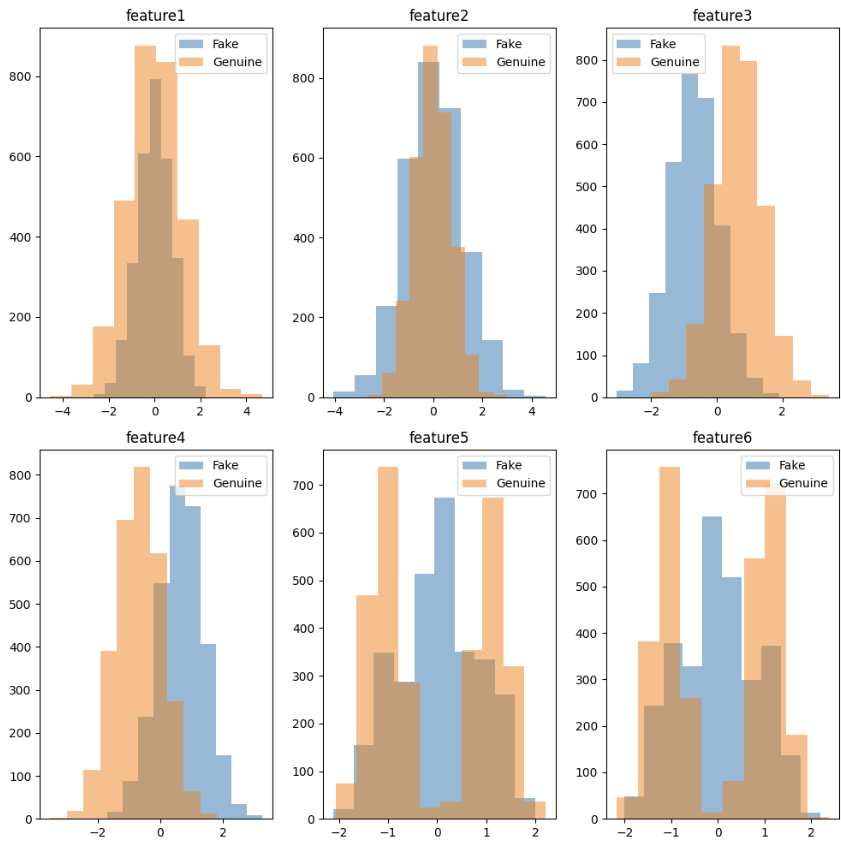
\includegraphics[width=0.5\textwidth]{./img/AllFeatures.png}
        \caption{All features}
        \label{fig:AllFeatures}
\end{figure}  
\\
By plotting a histogram for each feature, separately for the Fake and Genuine classes, it is possible to show whether the samples follow a Gaussian distribution and to what extent. 
Thus, we can say that some features follow a Gaussian distribution. Furthermore, it can be seen that features 4 and 5 may be the most discriminating features based on their ability to separate the data of the two classes.\\
\begin{figure}[ht]
    \begin{minipage}[b]{0.45\textwidth}
        \centering
        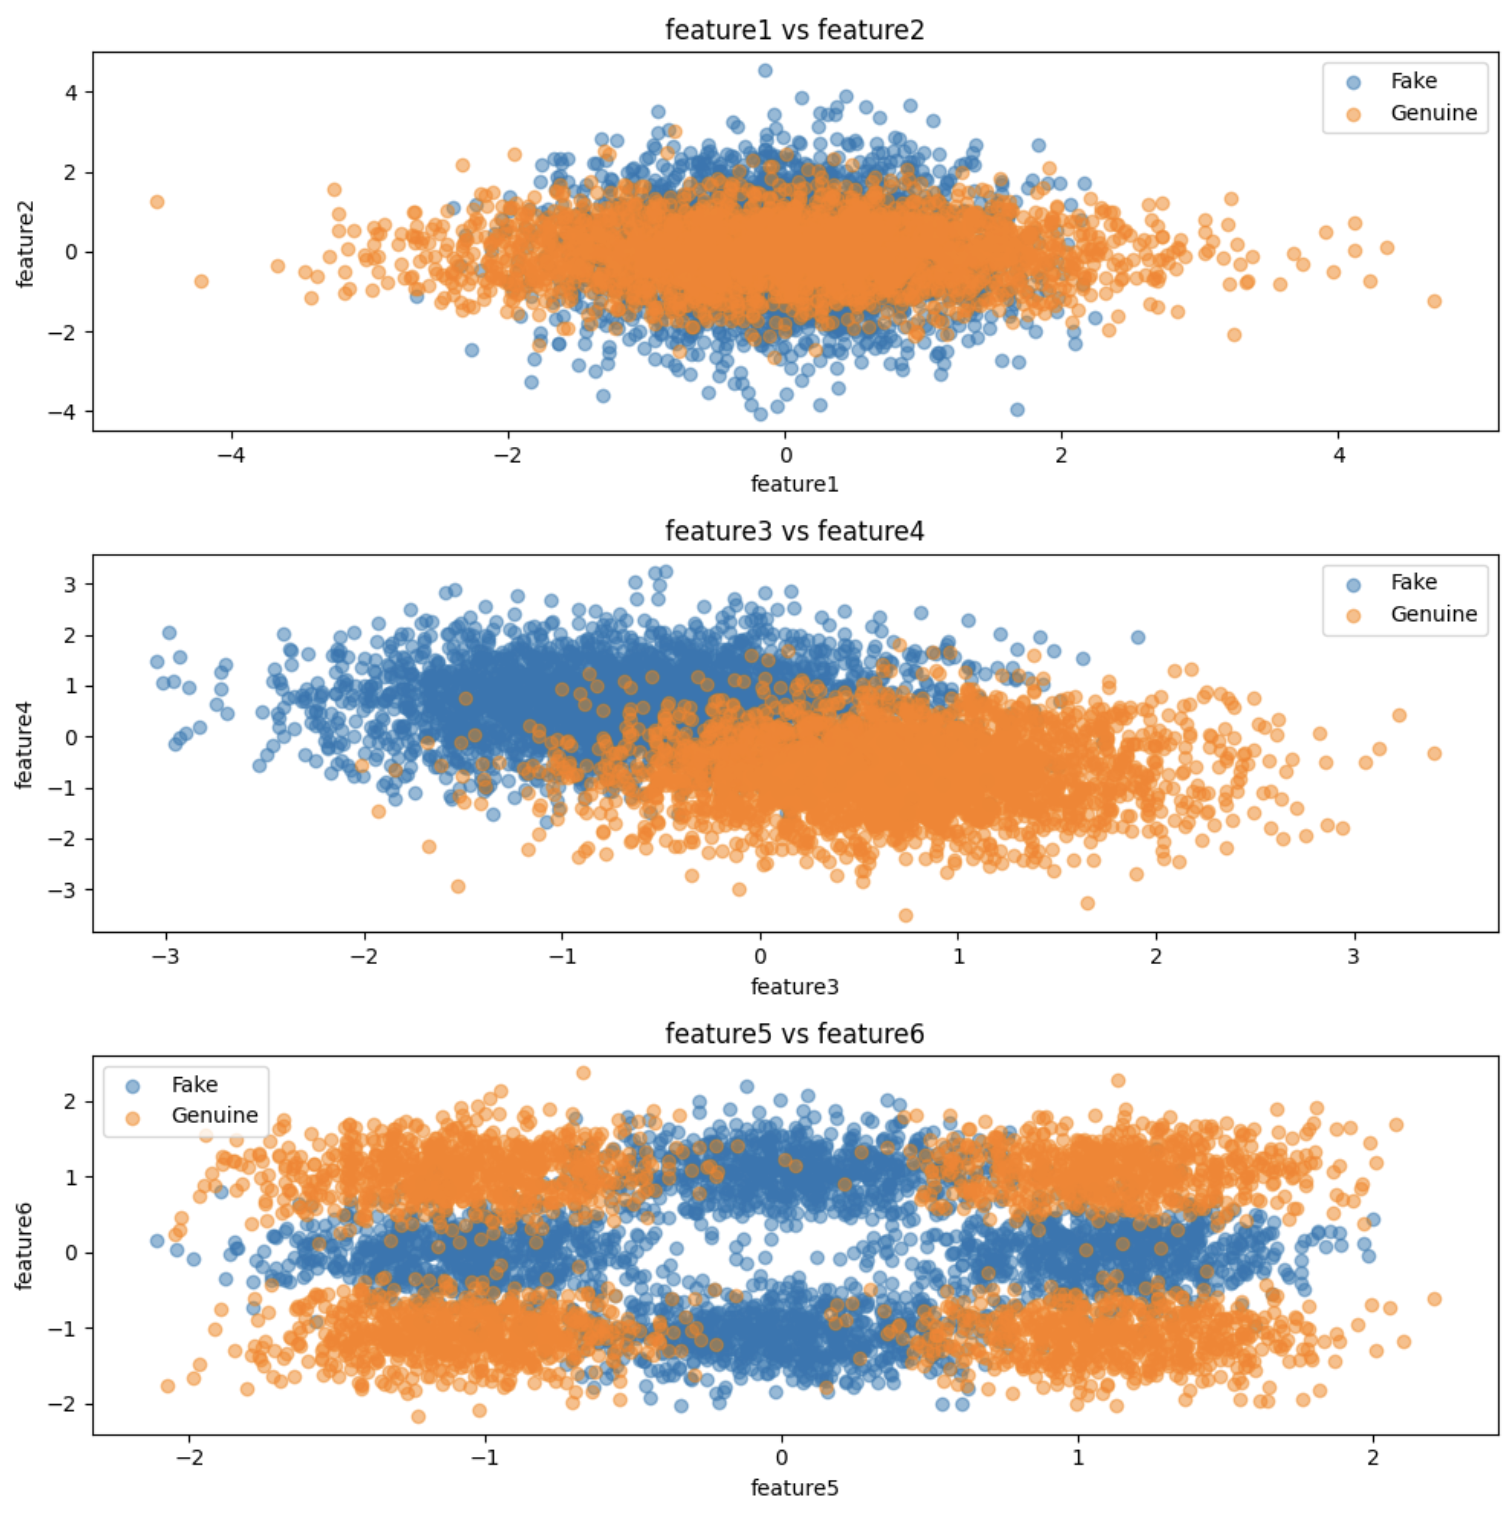
\includegraphics[width=\textwidth]{./img/image2.png}
        \caption{Distribution of feature pairs}
        \label{fig:PairFeatures}
    \end{minipage}
    \hfill % Aggiunge uno spazio orizzontale tra le due minipage se necessario
    \begin{minipage}[b]{0.45\textwidth}
        \centering
        \begin{tabular}{ccc}
            \hline
            Feature & Mean & Variance \\ \hline
            1 & 0.00170711 & 1.00134304 \\
            2 & 0.00503903 & 0.9983527 \\
            3 & -0.00560753 & 1.0024818 \\
            4 & 0.00109537 & 0.99029389\\
            5 & -0.00700025 & 1.00119747 \\
            6 & 0.00910515 & 0.99722374 \\ \hline
        \end{tabular}
        \caption{Mean and variance for each features}
        \label{tab:mean-variance}
    \end{minipage}
\end{figure}
    \\
After making these calculations we can conclude that the data are already centered since all features have mean close to zero.\\
Analyzing the pairwise averages and variances of the features, we can make some observations:  
\begin{itemize}
    \item Feature 1 and Feature 2: These two features have averages very close to zero, indicating that their values are similarly distributed around zero. However, the variance of Feature 2 is slightly lower than that of Feature 1, indicating that the values of Feature 2 are slightly less dispersed than those of Feature 1.  
    \item Feature 3 and Feature 4: Feature 3 has a negative mean, while Feature 4 has a positive mean. This might indicate that the values of Feature 3 tend to be lower than those of Feature 4. Also, the variance of Feature 3 is slightly higher than that of Feature 4, indicating that the values of Feature 3 are more dispersed than those of Feature 4.  
    \item Feature 5 and Feature 6: Feature 5 has a negative mean, while Feature 6 has a positive mean. This might indicate that the values of Feature 5 tend to be lower than those of Feature 6. Also, the variance of Feature 5 is slightly higher than that of Feature 6, indicating that the values of Feature 5 are more dispersed than those of Feature 6. 
\end{itemize}
\subsection{Features correlation}
We can show how correlated the features are by using a heatmap that shows a darker color within the cells for which there is a high correlation between feature i and feature j. The correlation between feature x and feature y is calculated using Pearson's coefficient:
\begin{equation}
    Corr_{i,j} = \frac{Cov(i,j)}{\sqrt{Var(i)}\sqrt{Var(j)}}  
\end{equation}
\begin{figure}[H]
    \centering
    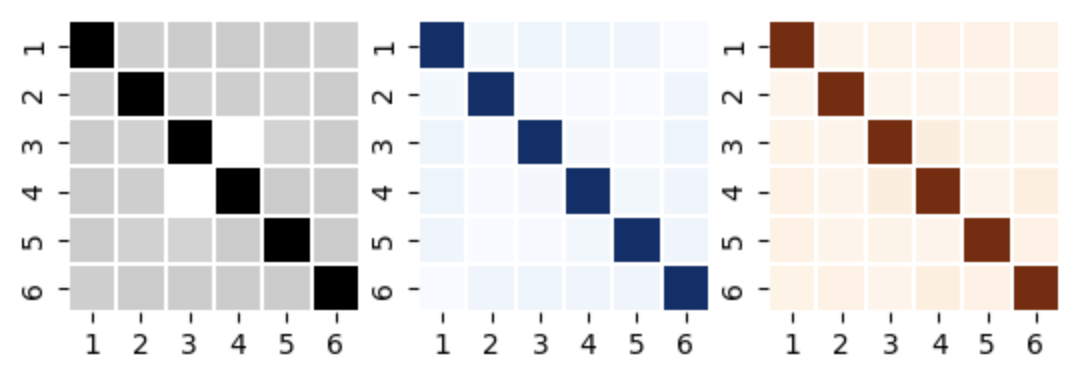
\includegraphics[width=0.8\textwidth]{./img/correlazione.png}
    \caption{Correlation features: gray scale indicates the correlation between whole dataset, blue is for Fake class and orange for Genuine class}
    \label{fig:AllFeatures}
\end{figure} 
Most of the features do not appear to be particularly correlated; in fact, most of the values in the correlation matrix are close to zero.\\
\\
Since the features do not appear to be strongly correlated since precisely the values are close to zero. This suggests to us that each feature carries unique information that could be useful for classification. Therefore, it is most likely that in PCA we will use a value of m as high as possible, possibly equal to the number of features in this way it will be possible to preserve as much of the information in the data as possible.\\
\\
While in the case of Naive Bayes model and Full Covariance Gaussian Model could have similar performance because the features appear to be not strongly correlated. While in the case of the Tied model, which shares the covariance matrix between the classes, it may not have very good performance since the features are not strongly correlated.

\section{Dimensionality reduction}
Dimensionality reduction is useful in this context to compute a mapping from an n-dimensional feature space to an m-dimensional space; it is applied because it can compress information, remove noise and simplify classification.
\subsection{PCA}
PCA is an unsupervised dimensionality reduction technique that, given a centered dataset \\\(X = \{x_1, \ldots, x_k\}\), it aims to find the subspace of \(R^n\) that allows to preserve most of the information, i.e. the directions with the highest variance.
We start by calculating the covariance matrix:
\begin{equation}
\mathbf{C} = \frac{1}{K} \sum_{i} (x_i - \bar{x})(x_i - \bar{x})^T
\end{equation}
After that we can compute the eigen-decomposition of \(
\mathbf{C} = \mathbf{U} \Sigma \mathbf{U}^T,
\)
where \( \mathbf{U} \) is the matrix of eigenvectors and \( \Sigma  \) is the diagonal matrix of eigenvalues. Now we can project the data into the new subspace, it is spanned by the m columns of U corresponding to the m values of the highest eigenvalues.\\
\begin{equation}
\mathbf{y_i} = \mathbf{P^T} (x_i - \bar{x})
\end{equation}
P is the matrix corresponding to the m columns of U associated with the m highest eigenvalues of C.
At this point to choose which is the best value of m we need to check how much total variance in the data we are able to retain using different values of m.
To do this evaluation, it was decided to represent on a graph the variance of the data as m increases, i.e., we exploited that each eigenvalue corresponds to the variance along the corresponding axis, and the eigenvalues are the elements of the diagonal of the matrix \(\Sigma\) . The percentage will be calculated as the ratio of the sum of the first m eigenvalues to the sum of all eigenvalues.
\begin{figure}[H]
    \centering
    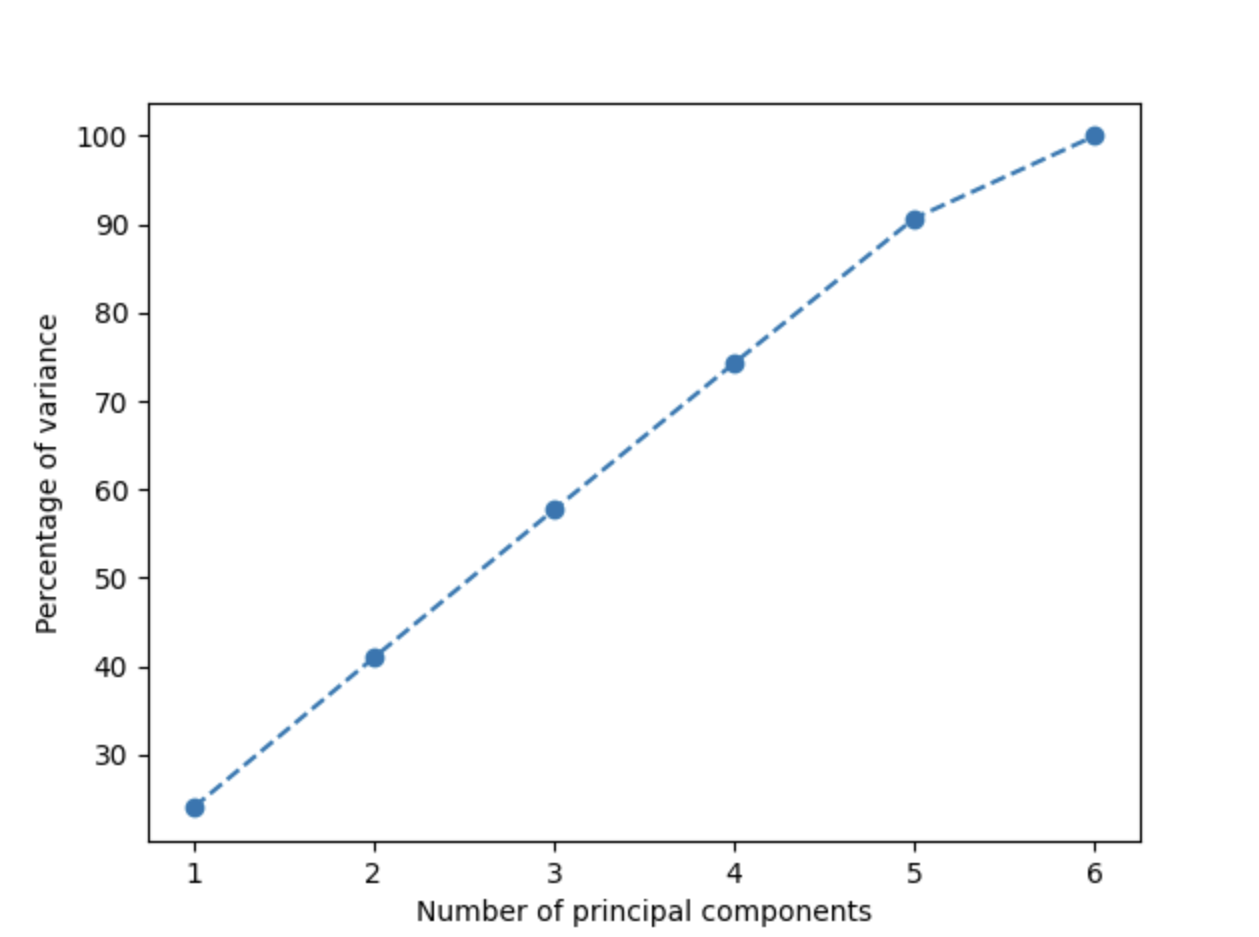
\includegraphics[width=0.5\textwidth]{./img/variance.png}
    \caption{Variance of data for each m values}
    \label{fig:variance}
\end{figure} 

It is clear from Figure~\ref{fig:variance} that values of \( m<5\) rapidly decrease the amount of variance retained in the data. Removing a feature is probably the best choice, since this way the percentage of variance remains fairly high.
\begin{figure}[H]
    \centering
    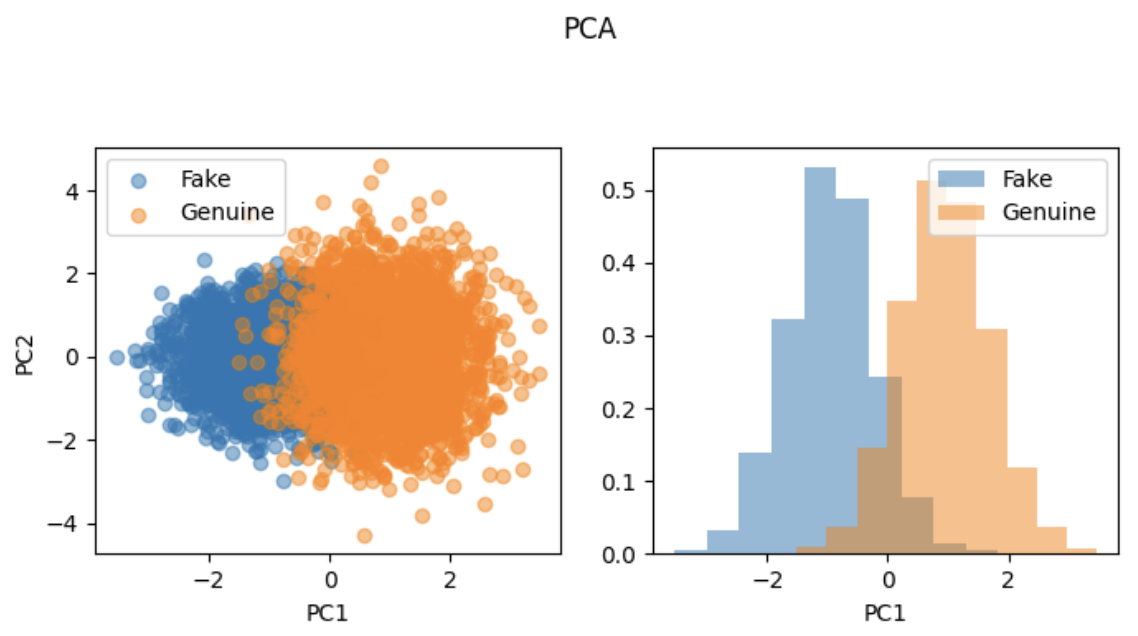
\includegraphics[width=0.7\textwidth]{./img/PCA.png}
    \caption{PCA for the two first components}
    \label{fig:PCA}
\end{figure} 

After the analysis done to choose which m is best to use, we can represent the first two principal components found by calculating the PCA with m=6, visualizing these components can help to understand which features contribute most to the variance in the data.
It can actually be observed that there is better separation between classes by applying PCA and choosing an m that has good variance of the data.
\subsection{LDA}
LDA is a supervised dimensionality reduction technique that aims to find the subspace that maximizes the separation between classes. \\
To compute the transformation matrix \( W \) we need to compute between-class and within-class covariance matrices.
\begin{equation}
\mathbf{S}_b =\frac{1}{N}\sum_{c=1}^{K} n_c (\mu_c - \mu)(\mu_c - \mu)^T
\end{equation}
\begin{equation}
    \mathbf{S}_w = \frac{1}{N}\sum_{c=1}^{K} \sum_{i=1}^{n_c} (x_{c,i} - \mu_i)(x_{c,i} - \mu_i)^T
    \end{equation}
where \( \mu_c \) is the mean of the c-th class, \( \mu \) is the mean of all the data, and \( n_c \) is the number of samples in the c-th class.\\
The LDA directions can be computed solving the generalized eigenvalue problem \(S_b w=\lambda S_w w\), usually to solve the generalized eigenvalue problem we transform the \(S_w\) matrix into an identity matrix and then solve the eigenvalue problem for the other \(S_b \) matrix. This process allows us to find the discriminant vectors \(w\) that maximize the separation between the classes.\\
In LDA, the maximum number of discriminant directions or dimensions that can be obtained is always equal to C-1 where C is the number of classes. This is because the goal of the LDA is to find the directions that maximize the separation between the classes. 
In our case having only two classes the LDA can find at most one direction that maximizes the separation between these two classes.
\begin{figure}[H]
    \centering
    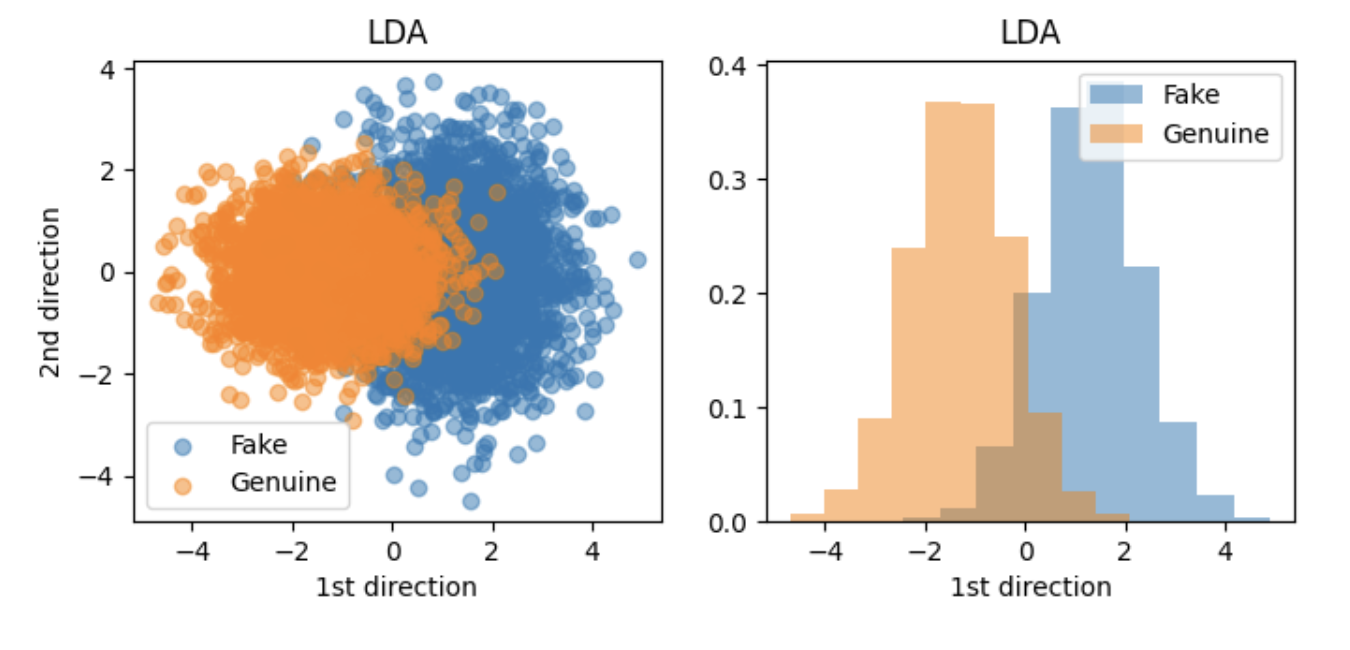
\includegraphics[width=0.7\textwidth]{./img/LDA.png}
    \caption{LDA for first direction}
    \label{fig:LDA}
\end{figure} 
Looking at the results of LDA, in Figure~\ref{fig:LDA}, we can see that it cannot find an optimal direction that gives us a better separation of classes than the results shown previously.
\subsection{Classification}
Subsequent to applying dimensionality reduction techniques we used LDA to perform classification, in fact after finding the hyperplane on the training data and projecting the validation data into the new space we used different thresholds to perform classification.
After applying dimensionality reduction techniques, we used LDA to perform classification; in fact, after finding the hyperplane on the training data and projecting the validation data into the new space these new data values can be used as scores by comparing them with different thresholds to perform classification, if the value exceeds the threshold it is associated with the label 1 while if it is lower 0.
Two different methods were used to calculate the threshold value:
\begin{itemize}

\item \textbf{First Threshold}: The first method calculates the average of the LDA values for the two classes and uses the average of these two averages as the threshold. This method is simpler, but does not take into account the distribution of the data or the classification error rate. In fact, it may not provide an optimal threshold if the data are not well balanced or if the distributions of the two classes overlap significantly.
\item \textbf{Second Threshold}: The second method uses a more sophisticated approach to determine the threshold. Instead of simply calculating the mean, a range of possible threshold values are examined and the one that minimizes the classification error rate is chosen. This method is more computationally heavy, but can lead to a more accurate threshold and a lower classification error rate.  
\end{itemize}
\begin{table}[H]
    \centering
    \begin{tabular}{lcc}
    \hline
    \textbf{Methods} & \textbf{Number of errors} & \textbf{Error rate (\%)} \\
    \hline
    LDA - First threshold & 275 & 13.75 \\
    LDA - Second threshold & 184 & 9.2 \\
    \hline
    PCA(m=6)+LDA - First threshold & 186 & 9.3 \\
    PCA(m=5)+LDA - First threshold & 186 & 9.3 \\
    PCA(m=6)+LDA - Second threshold & 184 & 9.2 \\
    PCA(m=5)+LDA - Second threshold & 185 & 9.25 \\
    \hline
    \end{tabular}
    \caption{LDA and PCA+LDA results with different threshold}
    \label{tab:resultsPCALDA}
\end{table}
As can be seen from the Table~\ref{tab:resultsPCALDA} there is not much real improvement by applying PCA as pre-processing before LDA and that the classification error turns out to be quite high so good classification is not performed using LDA or the combination of LDA with PCA.


\section{Multivariate Gaussian Density}
The multivariate Gaussian distribution is a generalization of the multidimensional Gaussian normal distribution. It is used to describe the probability of a vector of continuous random variables that can be correlated with each other.\\
The multivariate Gaussian distribution in d dimensions is characterized by a vector of averages \(\mu\)  and a covariance matrix \(\Sigma\). The probability density function of the multivariate Gaussian distribution is given by:
\begin{equation}
    \mathcal{N}(x|\mu,\Sigma ) = \frac{1}{(2\pi)^{M/2}|\Sigma|^{1/2}} \exp\left(-\frac{1}{2}(x-\mu)^T\Sigma^{-1}(x-\mu)\right)
\end{equation}
Very often to prevent numerical problems due to exponentiation of large numbers, it is usually recommended to work on the logarithm of the density:
\begin{equation}
    \log \mathcal{N}(x|\mu,\Sigma ) = - \frac{M}{2} \log(2\pi) -\frac{1}{2} \log |\Sigma| - \frac{1}{2}(x-\mu)^T\Sigma^{-1}(x-\mu) 
\end{equation}
\begin{figure}[H]
    \centering
    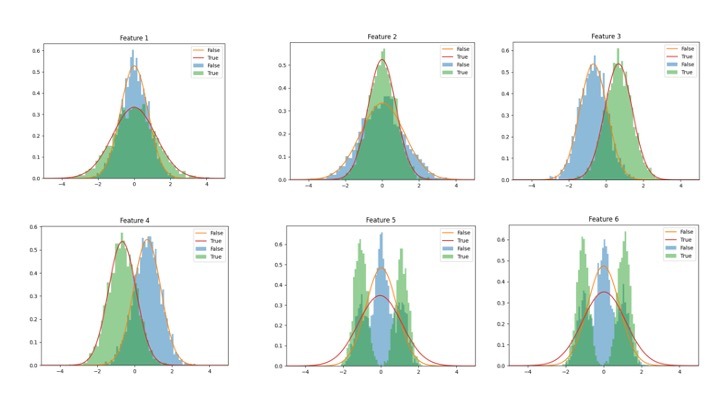
\includegraphics[width=0.8\textwidth]{./img/GaussianDensity.jpeg}
    \caption{Gaussian density}
    \label{fig:gaussianD}
\end{figure} 
The curve we can observe on the graph in Figure~\ref{fig:gaussianD} represents the Gaussian probability density calculated from the data. If the data actually follow a Gaussian distribution, then the curve should fit the histogram of the data well. When this happens we can say that the Gaussian model is a good fit for the data while if the Gaussian curve does not fit the histogram well, then the Gaussian model may not be the most appropriate model for that data.\\
We can observe that feature 1, feature 2, feature 3 and feature 4 fit the model well and follow a Gaussian distribution.
\section{Model evaluation for classification}
To understand which model is the most promising and gives us the best results, we divided the dataset as mentioned above into a part for training and a part for validation. This way we can test our model on data other than the training data.\\
We considered different types of applications i.e. various values of (\( \tilde{\pi},C_{fn},C_{fp})\). The target application chosen to be balanced will be:
\begin{equation}
    (\tilde{\pi},C_fp,C_fn) = (0.1,1,1)
\end{equation}
The objective of the following analysis is to choose the model with the best performance. Performance will be measured in terms of normalized minimum detection costs. This technique would allow us to discriminate the best performing model for our target application by providing an assessment of how well the model can detect the class to which it belongs. 
\\
It is defined as follows:
\begin{equation}
    DCF_u= \sum_{k=0}^{K-1} \frac{\pi_k}{N_k} \sum_{i|c_i=k}C(c_i^*|k)=\pi_TC_{fn} P_{fn}+(1-\pi_T)C_{fp}P_{fp} 
\end{equation}
\label{eq:DCF}
where \(P_{fn}=\frac{FN}{FN+FP}\) and \(P_{fp}=\frac{FP}{FP+TP}\).\\
\\
From the Equation~\ref{eq:DCF}  it is possible to find \textbf{minDCF} and \textbf{actDCF}, and different thresholds are used to calculate these. In fact in the case of minDCF one uses as a threshold the one that minimizes DCF and there are several methods to be able to find it. Whereas for actDCF you use as a threshold:
\begin{equation}
    t'=-\log{\frac{\tilde{\pi}}{1-\tilde{\pi}}}
\end{equation}

\section{Classification model analysis}
To perform the classification obviously we had to divide the training dataset into a part for training and a part for validation.

\subsection{Gaussian Models}
The first class of models we will analyze is that of Gaussian generative models. A simple model is to assume that our data, given a class, can be described by a Gaussian distribution:
\begin{equation}
    f_{x|C}(x|c) = \mathcal{N}(x|\mu_c,\Sigma_c)
\end{equation}
Since this is a binary classification task, we will assign a probability score to each sample in terms of the log-posterior class likelihood ratio:
\begin{equation}
    llr(x_t) = \log \;r(x_t) = \log \frac{P(C=h_1|x_t)}{P(C=h_0|x_t)}
\end{equation}
This expression can be expanded writing:
\begin{equation}
    llr(x_t) = \log \frac{f_{X|C}(x_t|C=h_1)}{f_{X|C}(x_t|C=h_1)} + \frac{\pi }{1-\pi }
\end{equation}
where \( f_{X|C}(x_t|c)=\mathcal{N}(x|\mu_c,\Sigma_c)\)\\\\
It is necessary to find the parameters \(\theta \), \(\mu_c\) and \(\Sigma_c \); this can be done by maximizing the log-likelihood.\\ Parameter estimation is part of the training phase and is therefore performed on the training part of the dataset.
While the estimation phase is to calculate the likelihood ratio for each sample and compare it to a threshold, which will be set at 0(th=0) in this step. After doing this, the error rate can be calculated to evaluate the classification. 
This analysis has been done on different Gaussian models, the difference between these models is the way the parameters \((\mu_c ,\Sigma_c )\) are calculated, more specifically \(\Sigma_c\).
\subsubsection{MVG Gaussian Classifier}
The first model we will analyze is the multivariate Gaussian classifier; in this model the covariance matrix is assumed to be different for each class. The parameters \(\mu_c\) and \(\Sigma_c\) are estimated by maximizing the log-likelihood of the training data. Thus they can be obtained as:
\begin{equation}
    \mu_c^* = \frac{1}{N_c} \sum_{i|c_i=C} x_{i} \;\;\;\;\; \Sigma_c^* = \frac{1}{N_c} \sum_{i|c_i=C} (x_{i} - \mu_c)(x_{i} - \mu_c)^T
\end{equation}
\subsubsection{Naive Bayes Classifier}
The Naive Bayes hypothesis simplifies the MVG full covariance model. In fact, if we know that the different components of our characteristics are approximately independent, we can simplify the estimation by assuming that the distribution of x|C can be factorized on its components.\\
The parameters then become:
\begin{equation}
    \mu_{c,[j]}^] = \frac{1}{N_c} \sum_{i|c_i=C} x_{i,[j]} \;\;\;\;\; \sigma_{c,[j]}^2 = \frac{1}{N_c} \sum_{i|c_i=C} (x_{i,[j]} - \mu_{c,[j]})^2
\end{equation}
The Naïve Bayes classifier corresponds to the MVG full covariance classifier with a diagonal covariance matrix.
\subsubsection{Tied Bayes Classifier}
Another common Gaussian Model is Tied Model, it assumes that the covariance matrix is the same for all classes, but each class still has its own mean.
It assumes that:
\begin{equation}
    f_{X|C}(x|c) = \mathcal{N}(x|\mu_c,\Sigma)
\end{equation}
While the parameters are estimated as:
\begin{equation}
    \mu_c^* = \frac{1}{N_c} \sum_{i|c_i=C} x_{i} \;\;\;\;\; \Sigma^* = \frac{1}{N} \sum_{c} \sum_{i|c_i=C} (x_{i} - \mu_c)(x_{i} - \mu_c)^T
\end{equation}
where \(N= \sum_{c=1}^{k}Nc\), that is the number of all samples.\\
This model is strongly related to LDA, if considering the binary log-likelihood ratio of the tied model we obtain a linear decision function:
\begin{equation}
    llr(x_t) = log \frac{f_{X|C}(x|h_1)}{f_{X|C}(x|h_0)}= x^Tb+c
\end{equation}
where b and c are functions of class means and covariance matrix. On the other hand, projecting
over the LDA subspace is, up to a scaling factor k, given by:
\begin{equation}
   w^tx=k x^T \Lambda (\mu_1-\mu_0)
\end{equation}

where \( \Lambda(\mu_1-\mu_0)=b\). The LDA assumption that all the classes have the same within class covariance matrix is related to the assumption done for the tied model.
\subsubsection{Gaussian Models Comparison}
At this point placing the \( P(C = 1) = P(C = 0) = 1/2\), classification was performed as can be seen in Table~\ref{tab:error_ratesMVG} using Gaussian models. 
\begin{table}[H]
    \centering
    \begin{tabularx}{0.6\textwidth}{>{\centering\arraybackslash}l>{\centering\arraybackslash}X>{\centering\arraybackslash}X} 
    \hline
    \textbf{Features} & \textbf{Model} & \textbf{Error Rate (\%)} \\
    \hline
    \multicolumn{3}{c}{no PCA} \\
    \hline
    1,2,3,4,5,6 & Full Cov & 7.00 \\
    1,2,3,4,5,6 & Naïve Bayes &  7.20 \\
    1,2,3,4,5,6 & Tied Cov &  9.30 \\
    \hline
    1,2,3,4 & Full Cov & 7.95 \\
    1,2,3,4 & Naïve Bayes &  7.65 \\
    1,2,3,4 & Tied Cov &  9.50 \\
    \hline
    1,2 & Full Cov &  36.50 \\
    1,2 & Naïve Bayes &  36.30 \\
    1,2 & Tied &  49.45 \\
    \hline
    3,4 & Full Cov &  9.45 \\
    3,4 & Naïve Bayes &  9.45 \\
    3,4 & Tied Cov &  9.40 \\
    \hline
    \multicolumn{3}{c}{PCA m= 5} \\
    \hline
    1,2,3,4,5,6 & Full Cov & 7.10 \\
    1,2,3,4,5,6 & Naïve Bayes & 8.75 \\
    1,2,3,4,5,6 & Tied Cov &  9.30 \\
    \hline
    \multicolumn{3}{c}{PCA m= 6} \\
    \hline
    1,2,3,4,5,6 & Full Cov &  7.00 \\
    1,2,3,4,5,6 & Naïve Bayes &  8.90 \\
    1,2,3,4,5,6 & Tied Cov &  9.30 \\
    \hline
    \end{tabularx}
    \caption{Error Rates for Different Models and Features}
    \label{tab:error_ratesMVG}
    \end{table}
Comparing the results with Table~\ref{tab:resultsPCALDA} , where LDA had been used for classification we can observe that for certain configurations there was an improvement. This could be due to the fact that this method is able to classify better and thus recognize the point to which class it belongs.
Analyzing the data provided in Table~\ref{tab:error_ratesMVG} we can make some considerations about the features used for classification:
\begin{itemize}
    \item \textbf{Features (1,2,3,4,5,6)}: the classification error is relatively low for all models, this may suggest that all features provide useful information.
    \item \textbf{Features (1,2,3,4)}: the classification error increases slightly, so it can be said that features 5 and 6 probably contain useful classification information.
    \item \textbf{Features (1,2),(3,4)}: the classification error increases significantly in the case of features(1,2) because they do not contain particularly important information for classification. While for (3,4),the error remains similar to the others , this might indicate that these two features are particularly informative for classification.  
\end{itemize}

Now we apply to estimate performance the metrics described in the previous section, we began by testing several applications to understand how changing parameters were reflected in performance. 
The prior value represents the a priori probability of the positive class, so if it is higher the value is expected to be more common, while a higher value of \(C_{fn}\) indicates that the cost of misclassifying a positive point as negative is higher, and vice versa for \(C_{fp}\).  
\begin{table}[H]
    \centering
    \begin{tabular}{>{\centering\arraybackslash}m{2cm} >{\centering\arraybackslash}m{2cm} >{\centering\arraybackslash}m{3cm}>{\centering\arraybackslash}m{2cm}}
    \hline
    \textbf{Model}  & \textbf{Full Cov} & \textbf{Naïve Bayes} & \textbf{Tied Cov} \\ \hline
    \rowcolor{yellow}
    \multicolumn{4}{c}{\textbf{Application(\(\pi_T,C_{fn},C_{fp}\)) : (0.50, 1, 1)}} \\   \hline
    \textbf{actDCF} & 0.139929 & 0.143929 & 0.186044 \\
    \textbf{minDCF} & 0.133016 & 0.131128 & 0.181244\\ \hline
    \rowcolor{yellow}
     \multicolumn{4}{c}{\textbf{Application(\(\pi_T,C_{fn},C_{fp}\)) : (0.90, 1, 1)}} \\   \hline
    \textbf{actDCF} & 0.400058 & 0.389257 & 0.462558 \\
    \textbf{minDFC} & 0.342309 & 0.350950 & 0.4421083 \\ \hline
    \rowcolor{yellow}
    \multicolumn{4}{c}{\textbf{Application(\(\pi_T,C_{fn},C_{fp}\)) : (0.10, 1, 1)}} \\   \hline
    \textbf{actDCF} & 0.304147 & 0.302163 & 0.405066 \\
    \textbf{minDFC} & 0.262913 & 0.256960 & 0.364823 \\ \hline

    \multicolumn{4}{c}{\textbf{Application(\(\pi_T,C_{fn},C_{fp}\)) : (0.50, 1, 9)}} \\   \hline
    \textbf{actDCF} & 0.305140 & 0.302163 & 0.406058 \\
    \textbf{minDFC} & 0.262913 & 0.256960 & 0.362839 \\ \hline

    \multicolumn{4}{c}{\textbf{Application(\(\pi_T,C_{fn},C_{fp}\)) : (0.50, 9, 1)}} \\   \hline
    \textbf{actDCF} & 0.400058 & 0.389257 & 0.462558 \\
    \textbf{minDFC} & 0.342309 & 0.350950 & 0.445132 \\ \hline
    \end{tabular}
    \caption{minDCF and actDCF for Different Models and configurations}
    \label{tab:model_comparison}
    \end{table}
    So it can be seen from the Table~\ref{tab:model_comparison} that:
    \begin{itemize}
        \item When the value of Prior increases (from 0.50 to 0.90), a worsening of the models can be seen. This is due to the fact that the model is penalizing false negatives more heavily. This also happens when Prior decreases(from 0.50 to 0.10) and therefore you are penalizing false positives more heavily.
        \item When \(C_{fp}\) or \(C_{fn}\) increase to 9.00, the actDCF and minDCF of all models worsen compared with the case when \(C_{fp}\) and \(C_{fn}\) were 1.00. However, it is possible to see the increase in the cost of false positives has less significant impact on the performance of the model so this suggests that the increase in the cost of false positives affects the model less.  While in the case of the cost of false negatives this has a higher impact so from this it can be inferred that increasing the cost of false negatives worsens the performance of the models.
    \end{itemize}
We now focus on the three applications that have different effective priors (0.1, 0.5, 0.9) and with costs of errors equal to 1.00 and we can, we can consider PCA as pre-processing.\\
\begin{table}[H]
\centering
\begin{tabular}{>{\centering\arraybackslash}m{2cm} >{\centering\arraybackslash}m{2cm} >{\centering\arraybackslash}m{3cm}>{\centering\arraybackslash}m{2cm}}
\hline
\textbf{Model}  & \textbf{Full Cov} & \textbf{Naïve Bayes} & \textbf{Tied Cov} \\ \hline\hline
\multicolumn{4}{c}{\textbf{Application(\(\pi_T,C_{fn},C_{fp}\)) : (0.50, 1, 1)}} \\   \hline
\multicolumn{4}{c}{\textbf{no PCA}}\\  \hline
\textbf{actDCF} & 0.139929 & 0.143929 & 0.186044 \\
\textbf{minDCF} & 0.133016 & 0.131128 & 0.181244\\ \hline
\multicolumn{4}{c}{\textbf{PCA}}\\  \hline
\multicolumn{4}{c}{m=5}\\  \hline
\textbf{actDCF} & 0.141913 & 0.174987 & 0.186044 \\
\textbf{minDCF} & 0.133144 & 0.173691 & 0.181163\\ \hline
\multicolumn{4}{c}{m=6}\\  \hline
\textbf{actDCF} & 0.139929 & 0.177995 & 0.186028 \\
\textbf{minDCF} & 0.130168 & 0.172699 & 0.181244\\ \hline\hline

\multicolumn{4}{c}{\textbf{Application(\(\pi_T,C_{fn},C_{fp}\)) : (0.90, 1, 1)}} \\   \hline
\multicolumn{4}{c}{\textbf{no PCA}}\\  \hline
\textbf{actDCF} & 0.400058 & 0.389257 & 0.462558 \\
\textbf{minDFC} & 0.342309 & 0.350950 & 0.4421083 \\ \hline
\multicolumn{4}{c}{\textbf{PCA}}\\  \hline
\multicolumn{4}{c}{m=5}\\  \hline
\textbf{actDCF} & 0.398041 & 0.466014 & 0.462558 \\
\textbf{minDCF} & 0.351238 & 0.434044 & 0.445132 \\ \hline
\multicolumn{4}{c}{m=6}\\  \hline
\textbf{actDCF} & 0.400058 & 0.451181 &  0.462558\\
\textbf{minDCF} & 0.342309 & 0.435915 & 0.442108\\ \hline\hline

\multicolumn{4}{c}{\textbf{Application(\(\pi_T,C_{fn},C_{fp}\)) : (0.10, 1, 1)}} \\   \hline
\multicolumn{4}{c}{\textbf{no PCA}}\\  \hline
\textbf{actDCF} & 0.304147 & 0.302163 & 0.405066 \\
\textbf{minDFC} & 0.262913 & 0.256960 & 0.364823 \\ \hline
\multicolumn{4}{c}{\textbf{PCA}}\\  \hline
\multicolumn{4}{c}{m=5}\\  \hline
\textbf{actDCF} & 0.304147 & 0.393017 & 0.405066 \\
\textbf{minDFC} & 0.273825 & 0.354470 & 0.364823 \\ \hline
\multicolumn{4}{c}{m=6}\\  \hline
\textbf{actDCF} & 0.305140 & 0.392025 & 0.406058 \\
\textbf{minDCF} & 0.262913 & 0.353479 & 0.362839\\ \hline
\end{tabular}
\caption{minDCF and actDCF for Different Models and configurations with and without PCA}
\label{tab:model_chooseApp}
\end{table}
\begin{itemize}
    \item From this first analysis, we can infer that the worst model is Tied Covariance (Tied Cov), as we had already assumed by analyzing the correlation of features since in this model the features are assumed to be correlated and in our case they are not strongly correlated.
\item We can see that after applying PCA, actDCF and minDCF remain unchanged or in some cases even worsen, which could indicate that the reduction in dimensionality removed some important information from the data that was useful for classification. That is, the components (or dimensions) that have been removed might contain discriminative information that helps the model distinguish between classes, or the transformation might break the assumptions made for the models under analysis and thus we might get an inaccurate estimate that worsens performance.
\item According to different applications the full Covariance and naive bayes model have similar performance, however, both have some strengths and weaknesses.
The Full Covariance model considers all correlations between features, so it may be able to capture more complex relationships between features, but this may lead to overfitting and also may be computationally heavier. On the other hand, on the other hand, the Naive Bayes model assumes that all features are independent of each other which might not be entirely true in our situation but it gets us good performance and might be a simplification, this however is less computationally heavy.
\item The application that has the best calibration, that is, where minDCF and actDCF are as close as possible is the one with the \(\pi_T=0.5\) both in the case where there is no pca application and the one where there is. In this case we can say that there is a good calibration for almost all models, while in the case of the other priors there is no good calibration.
\end{itemize}
    
\begin{figure}[H]
    \centering
    \begin{minipage}{.3\textwidth}
        \centering
        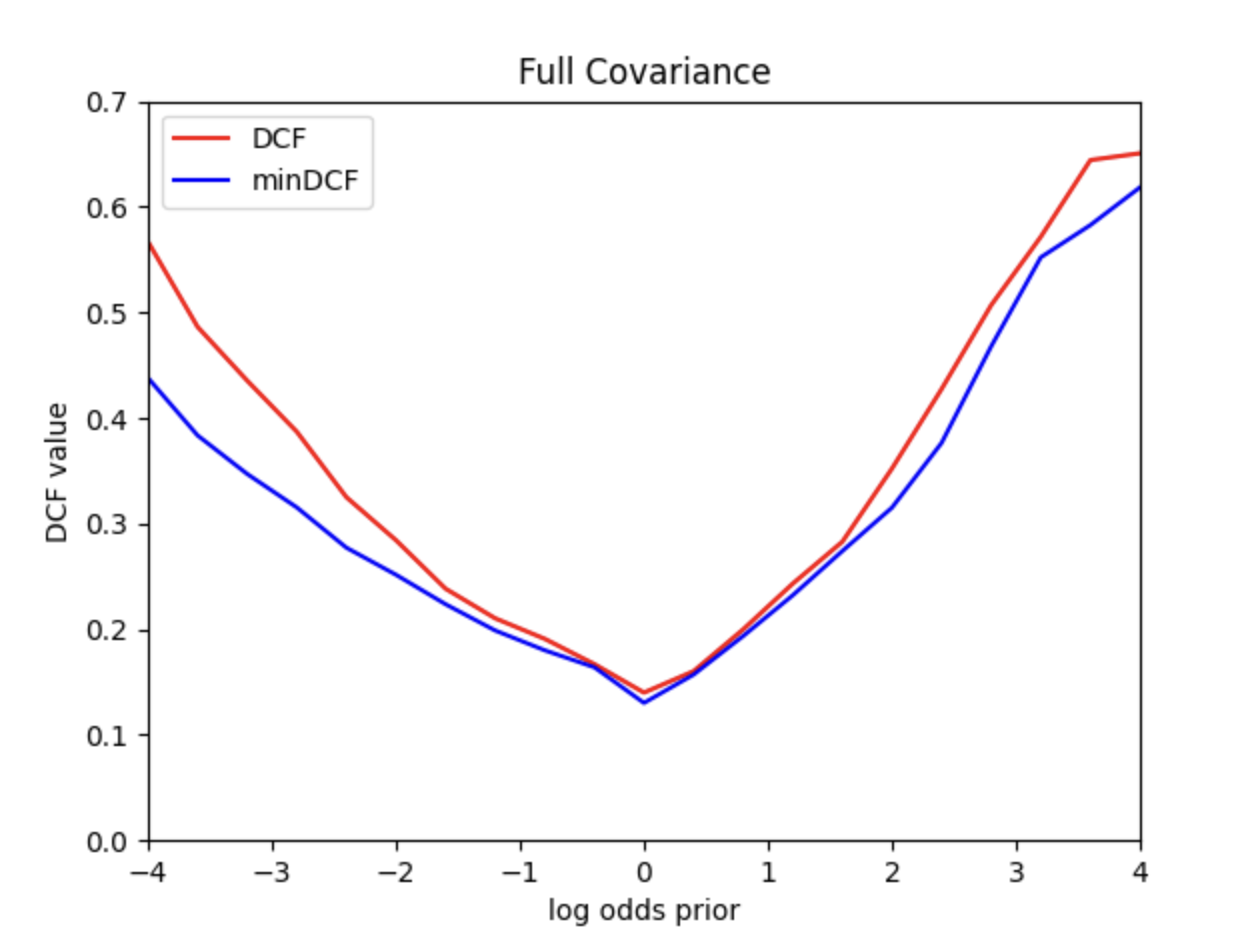
\includegraphics[width=\linewidth]{./img/full.png}
        % Rimuovi la caption e l'etichetta da qui
    \end{minipage}%
    \begin{minipage}{.3\textwidth}
        \centering
        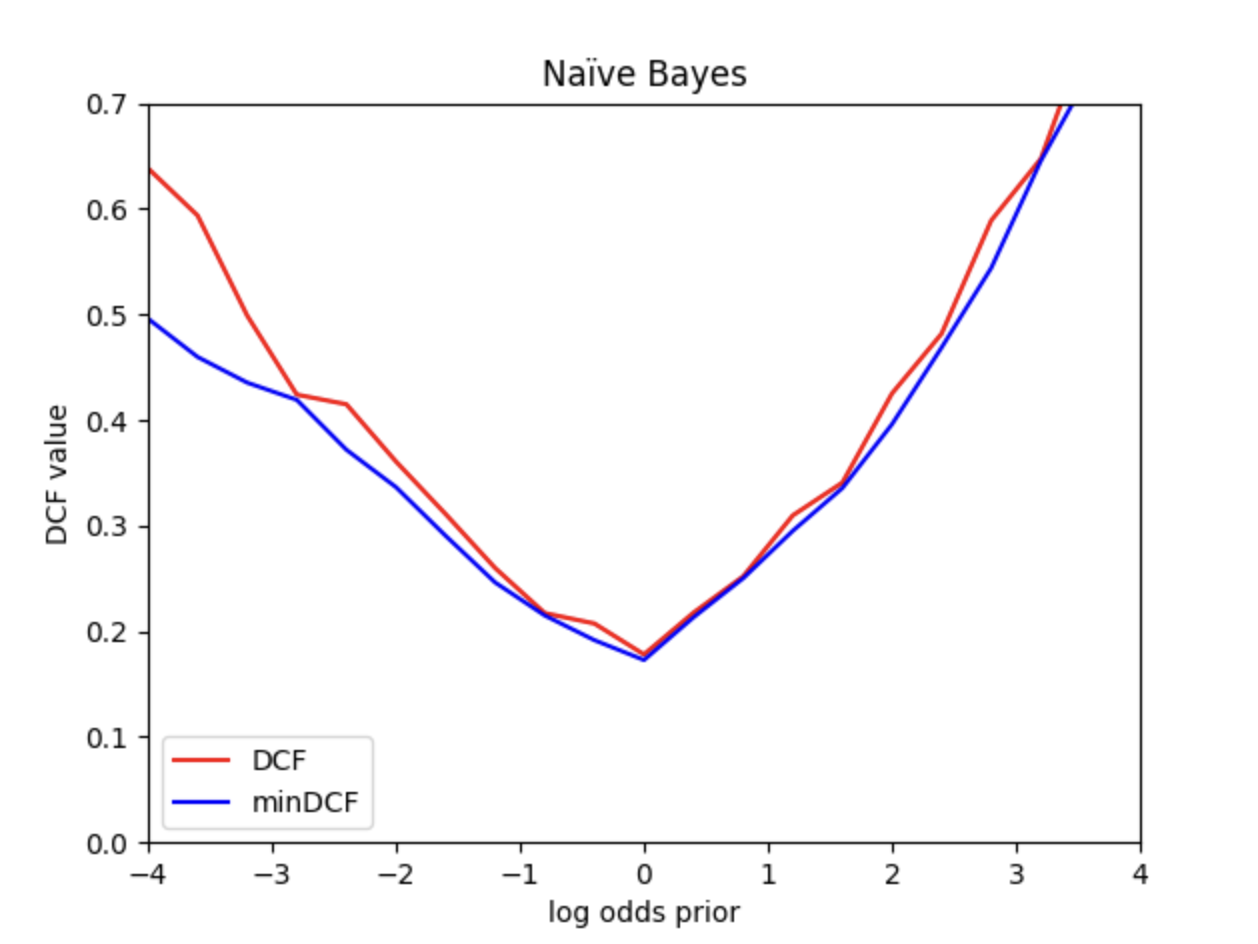
\includegraphics[width=\linewidth]{./img/naive.png}
        % Rimuovi la caption e l'etichetta da qui
    \end{minipage}
    \begin{minipage}{.3\textwidth}
        \centering
        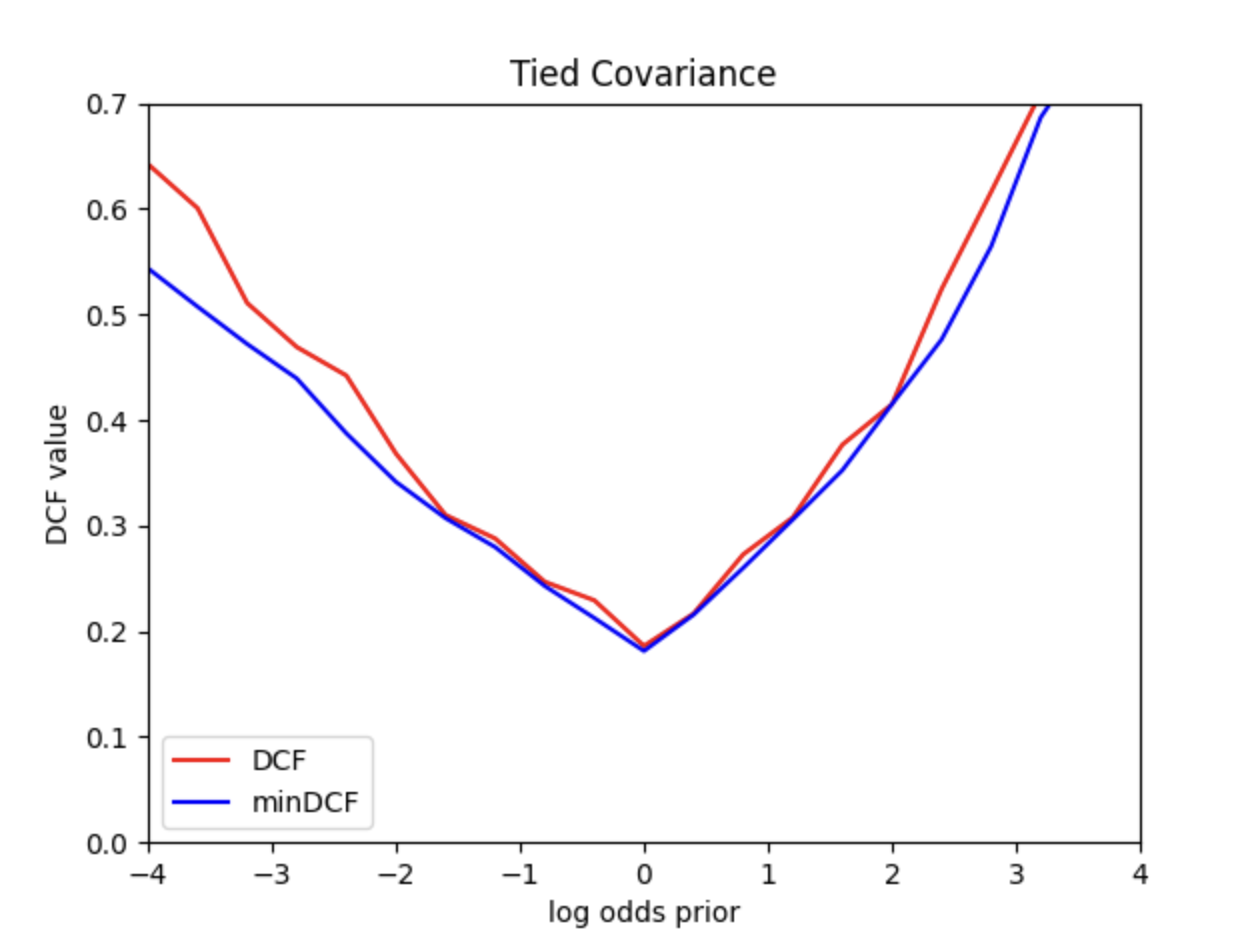
\includegraphics[width=\linewidth]{./img/tied.png}
        % Rimuovi la caption e l'etichetta da qui
    \end{minipage}
    \caption{Confronto tra i modelli: Full Covariance, Naive Bayes, e Tied Covariance} % Aggiungi una caption unica qui
    \label{fig:models_comparison} % Aggiungi un'etichetta unica qui
\end{figure}
\underline{Best Gaussian Model} analyzed for our main application that is application with \(\pi_T=0.1\) is:
\begin{itemize}
    \item \textbf{PCA}: Model Full Covariance with PCA(m=6)
    \item \textbf{No PCA}: Model Naive Bayes 
\end{itemize}
\subsection{Logistic Regression Classifier}
Logistic Regression is a discriminative classification model that makes no assumptions about the distribution of the data, but tries to find a hyperplane that maximizes the posterior likelihood. 
Starting from the results obtained from the Tied Gaussian that provides log-likelihood ratios that are linear functions of our data we can write it as:
\begin{equation}
    llr(x) =\log{\frac{P(C=h_1|x)}{P(C=h_0|x)}}=\log{\frac{f_{X|C}(x|h_1)}{f_{X|C}(x|h_0)}}+\log{\frac{\pi}{1-\pi}}= w^Tx + b
\end{equation}
All prior information has been absorbed in the bias term b, given w and b we can compute the expression for the posterior class probability:
\begin{equation}
    P(C=h_1|x,w,b)=\frac{e^{(w^Tx+b)}}{1+e^{(w^Tx-b)}}=\sigma(w^Tx+b)
\end{equation}
where \(\sigma=\frac{1}{1-e^{-x}}\) is the sigmoid function.\\
This equation provides a model that allows computing the posterior prabilities for h1 and h0, the model assumes that decision rules are linear surfaces orthogonal to the vector \textbf{w} and the model parameters are \((\textbf{w},b)\).
\subsubsection*{Training Model with centered data}
We used z-normalization to see how performance could change by applying normalization to the data, this was applied as prepocessing to Binary Logistic Regression and paired with the application of PCA.
\subsubsection{Binary Logistic Regression}
\subsubsection*{Binary Logistic Regression non prior-weighted}
We are going to look for the minimizer of the function:
\begin{equation}
    \mathbf{J}(w,b)=\frac{\lambda}{2} ||w||^2 + \frac{1}{n} \sum_{i=1}^{n} \log({1+e^{-z_i(w^Tx_i+b)}}),\;\;\;\;
        z_i = 
        \begin{cases} 
          1 & \text{if } c_i=1 \\
          -1 & \text{if } c_i=0
        \end{cases}
\end{equation}
where \(\lambda\)  is an hyperparameter that represents the regularization term (or norm penalty), that has been introduced to make the problem solvable in case of linearly separable classes.\\
\\
\begin{figure}[H]
    \centering
    \begin{minipage}{.27\textwidth}
        \centering
        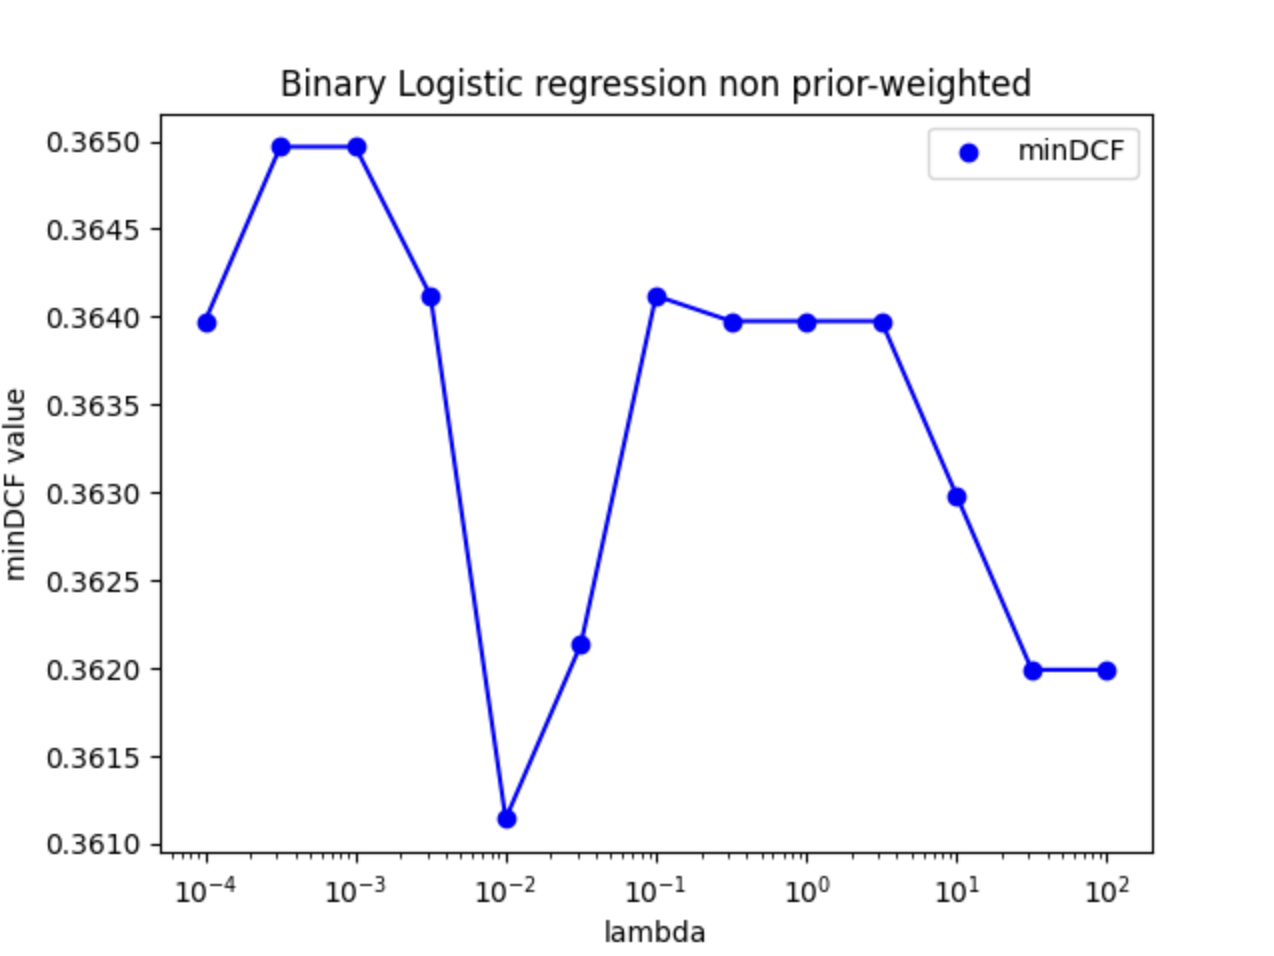
\includegraphics[width=\linewidth]{./img/LLR_noW1.png}
    \end{minipage}%
    \begin{minipage}{.27\textwidth}
        \centering
        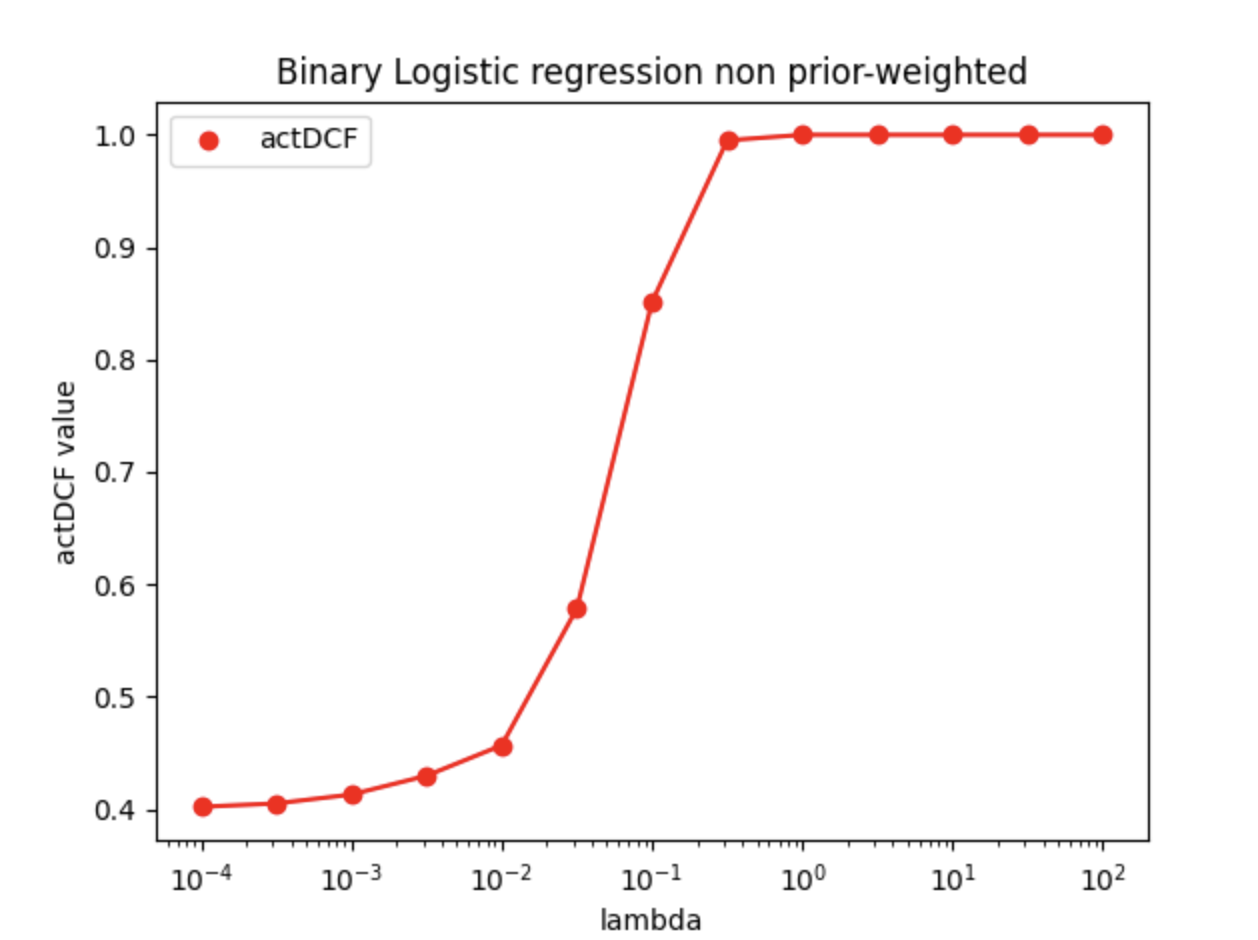
\includegraphics[width=\linewidth]{./img/LLR_noW2.png}
    \end{minipage}%
    \begin{minipage}{.27\textwidth}
        \centering
        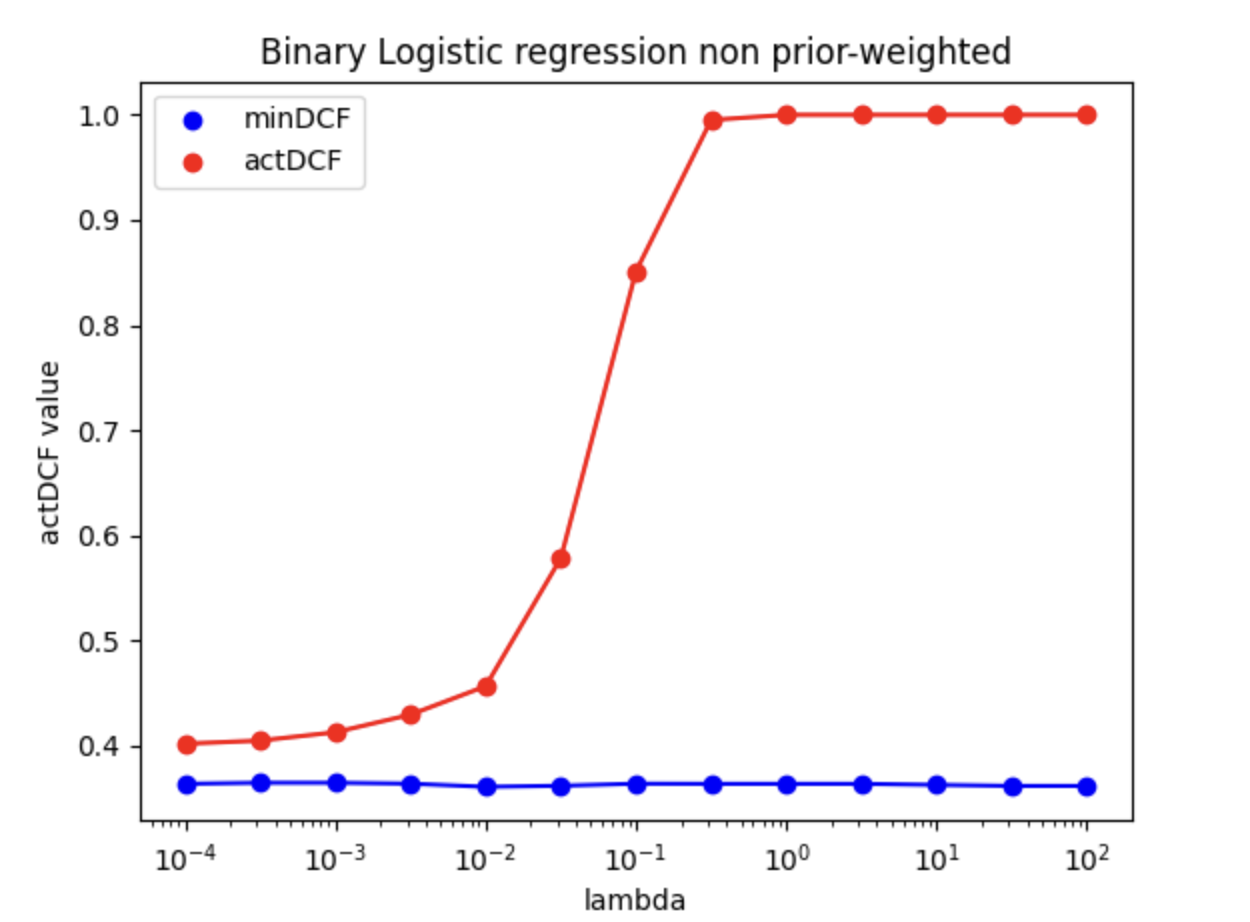
\includegraphics[width=\linewidth]{./img/LLR_noW3.png}
    \end{minipage}%
    \begin{minipage}{.25\textwidth}
        \centering
        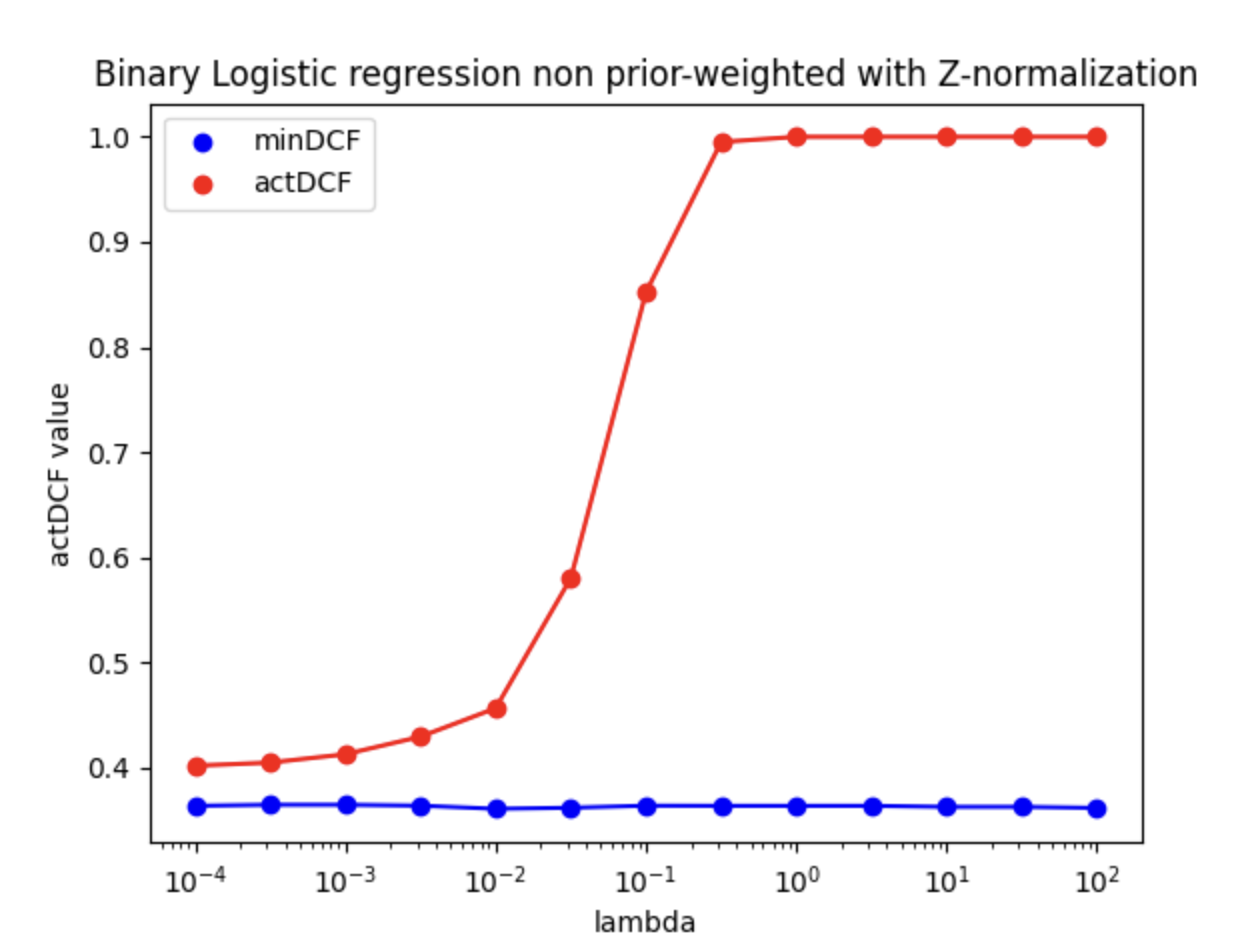
\includegraphics[width=\linewidth]{./img/LLR_Z1.png} % Aggiungi il percorso della tua quarta immagine qui
    \end{minipage}
    \caption{Binary Logistic Regression Model non prior-weighted}
    \label{fig:LLR_model}
\end{figure}
    \begin{figure}[H]
        \centering
        \begin{minipage}{.3\textwidth}
            \centering
            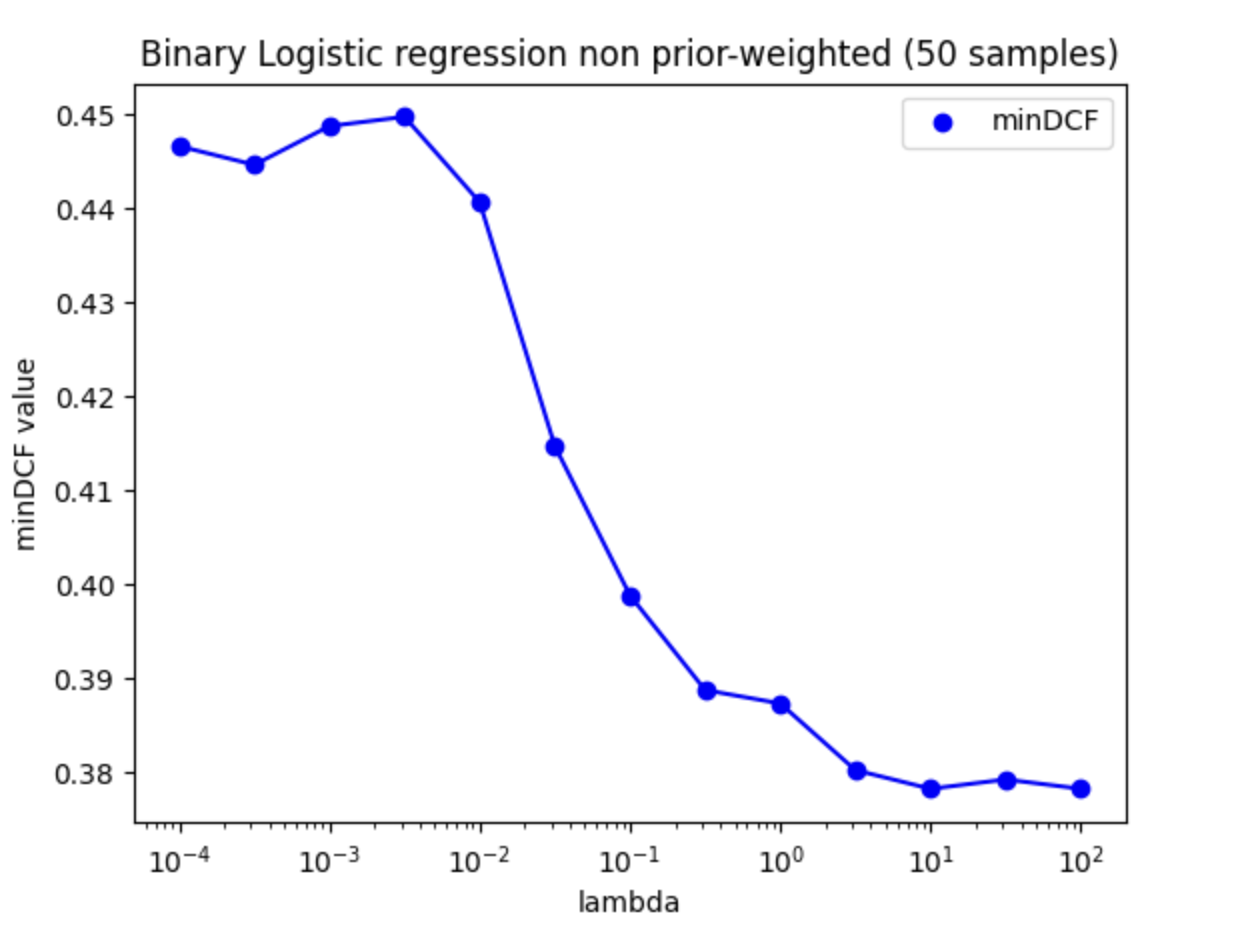
\includegraphics[width=\linewidth]{./img/LLR_noW501.png}
            % Rimuovi la caption e l'etichetta da qui
        \end{minipage}%
        \begin{minipage}{.3\textwidth}
            \centering
            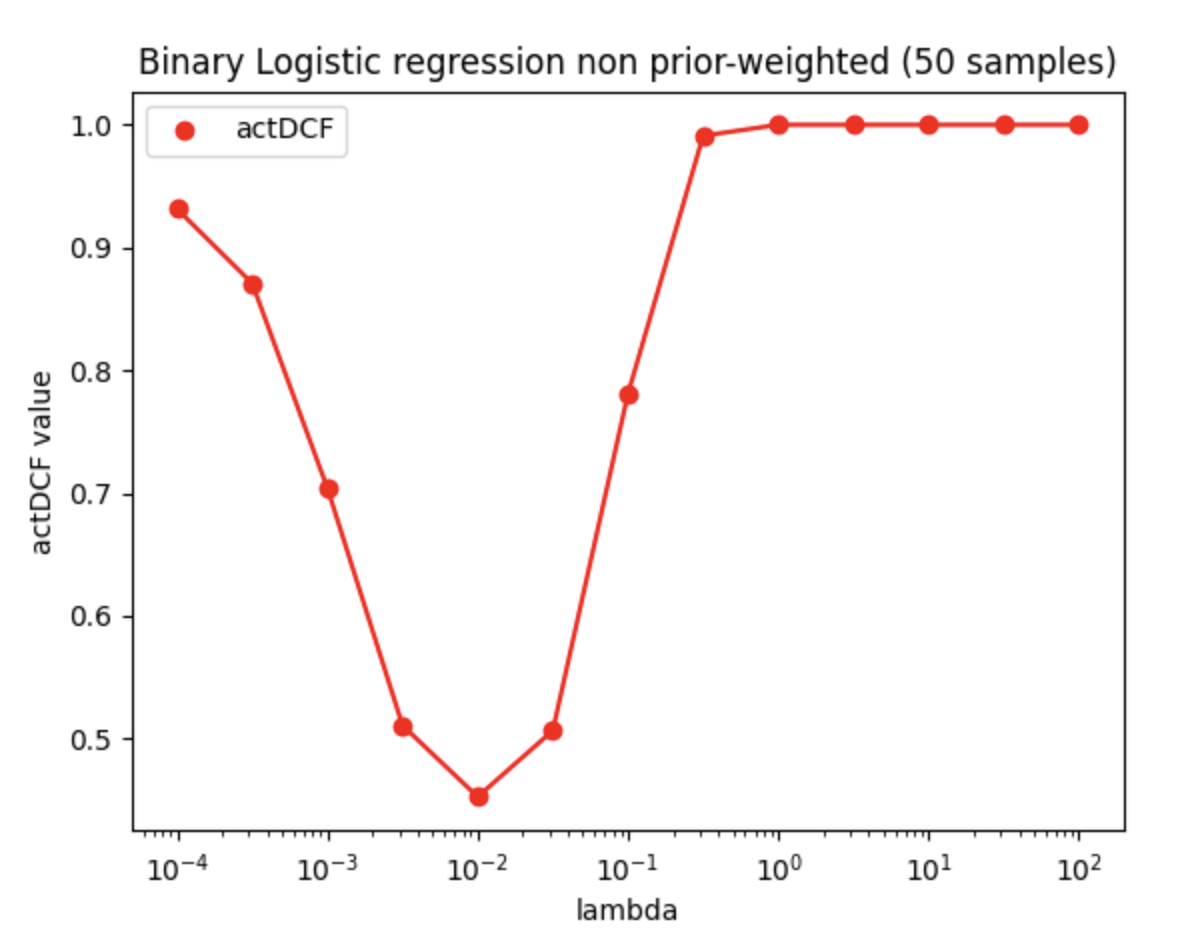
\includegraphics[width=\linewidth]{./img/LLR_noW502.png}
            % Rimuovi la caption e l'etichetta da qui
        \end{minipage}
        \begin{minipage}{.3\textwidth}
            \centering
            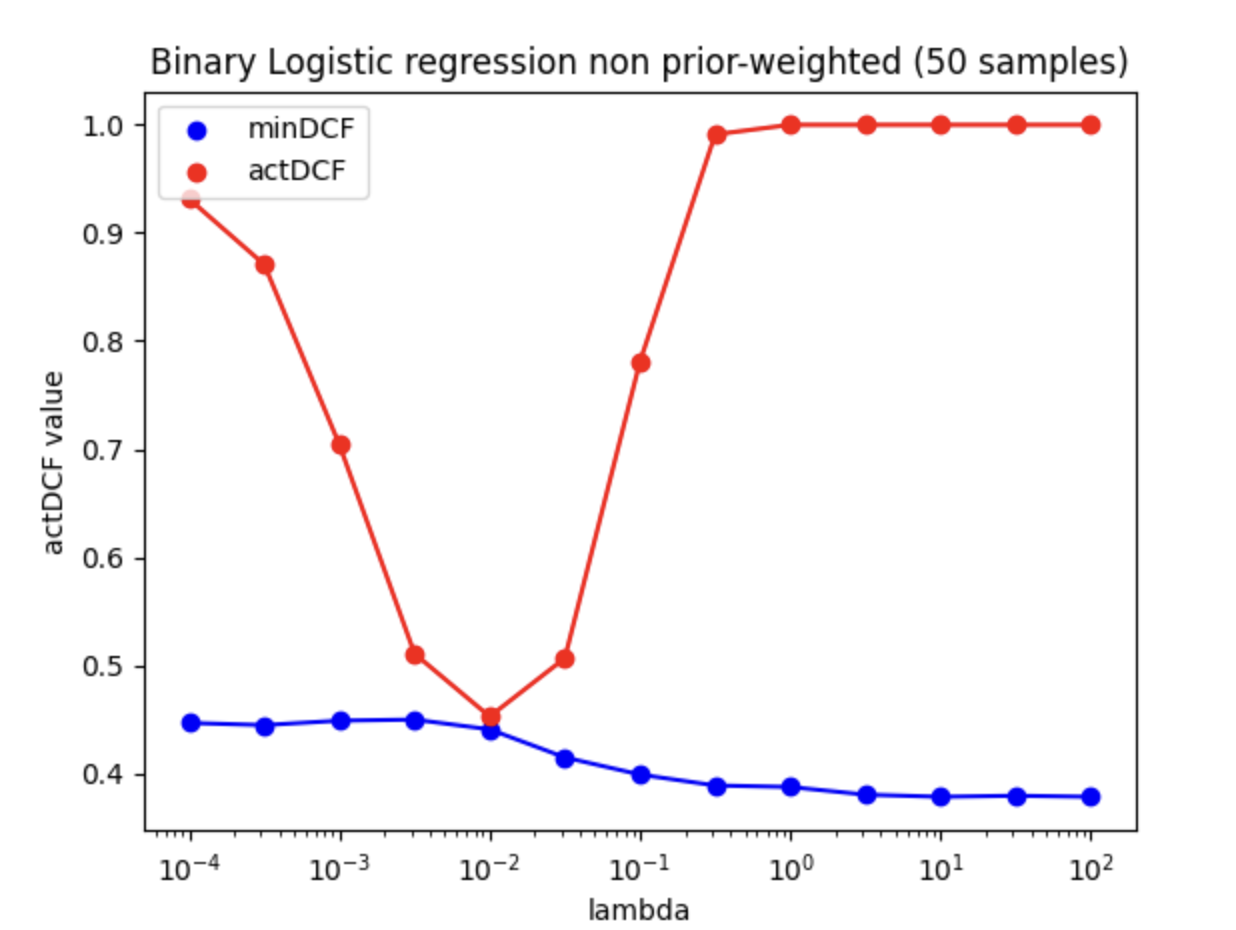
\includegraphics[width=\linewidth]{./img/LLR_noW503.png}
            % Rimuovi la caption e l'etichetta da qui
        \end{minipage}
        \caption{Binary Logistic Regression Model non prior-weighted(50 samples)} % Aggiungi una caption unica qui
        \label{fig:LLR_model_50} % Aggiungi un'etichetta unica qui
    \end{figure}
    Now we can analyze the results of the binary logistic regression model on the primary application \(\pi_T=0.1\).
    % \begin{table}[H]
    %     \centering
    %     \begin{tabular}{>{\centering\arraybackslash}m{2cm} >{\centering\arraybackslash}m{3cm}>{\centering\arraybackslash}m{2cm}}
    %     \hline
    %     \textbf{\(\lambda\)}  &  \textbf{minDCF} & \textbf{actDCF} \\ \hline\hline
    %     \multicolumn{3}{c}{\textbf{Binary Logistic Regression non prior-weighted model}} \\   \hline
    %     \textbf{\(10^{-4}\)} &  0.363975 & 0.402089 \\
    %     \textbf{\(10^{-3}\)} & 0.364967 & 0.413002 \\
    %     \textbf{\(10^{-2}\)} & \textcolor{red}{0.361143} & 0.413002 \\
    %     \textbf{\(10^{-1}\)} &  0.364119 & 0.851190 \\\hline\hline
    %     \multicolumn{3}{c}{\textbf{Binary Logistic Regression non prior-weighted (50 samples)}} \\   \hline
    %     \textbf{\(10^{-4}\)} & 0.446604 & 0.93146\\
    %     \textbf{\(10^{-3}\)} & 0.448733 & 0.704077 \\
    %     \textbf{\(10^{-2}\)} & 0.440652 & 0.452557\\
    %     \textbf{\(10^{-1}\)} & 0.398842 & 0.780898\\\hline
    %     \end{tabular}
    %     \caption{minDCF and actDCF}
    %     \label{tab:LLR}
    %     \end{table}
    \begin{table}[H]
        \centering
        \begin{tabular}{>{\centering\arraybackslash}m{1cm} >{\centering\arraybackslash}m{2cm} >{\centering\arraybackslash}m{2cm} >{\centering\arraybackslash}m{2cm} >{\centering\arraybackslash}m{2cm}}
        \hline
        \multicolumn{5}{c}{\textbf{Binary Logistic Regression non prior-weighted model}} \\ \hline
        \textbf{\(\lambda\)} & \multicolumn{2}{c}{\textbf{minDCF}} & \multicolumn{2}{c}{\textbf{actDCF}} \\ \cline{2-5} 
         & \textbf{no z-norm} & \textbf{z-norm} & \textbf{no z-norm} & \textbf{z-norm} \\ \hline
        \textbf{\(10^{-4}\)} & 0.363975 &  0.363975 & 0.402089 & 0.402089 \\
        \textbf{\(10^{-3}\)} & 0.364967 & 0.364967 & 0.413002 & 0.413002 \\
        \textbf{\(10^{-2}\)} & \textcolor{red}{0.361143} & 0.361143 & 0.413002 & 0.456781 \\
        \textbf{\(10^{-1}\)} & 0.364119 & 0.364119 & 0.851190 & 0.852182 \\ \hline\hline
        \end{tabular}
        
        \begin{tabular}{>{\centering\arraybackslash}m{3cm} >{\centering\arraybackslash}m{3cm}>{\centering\arraybackslash}m{3cm}}
        \multicolumn{3}{c}{\textbf{Binary Logistic Regression non prior-weighted (50 samples)}} \\   \hline
        \textbf{\(\lambda\)} & \textbf{minDCF} & \textbf{actDCF} \\ \hline
        \textbf{\(10^{-4}\)} & 0.446604 & 0.93146\\
        \textbf{\(10^{-3}\)} & 0.448733 & 0.704077 \\
        \textbf{\(10^{-2}\)} & 0.440652 & 0.452557\\
        \textbf{\(10^{-1}\)} & 0.398842 & 0.780898\\\hline
        \end{tabular}
        \caption{minDCF and actDCF}
        \label{tab:LLR}
    \end{table}
        \begin{itemize}
            \item Using only 50 samples, we can see that using a limited number of samples can significantly affect the logistic regression model and could lead to misleading outcomes that are not 
                representative of the entire dataset. 
                In fact, the \(\lambda\) values for which we get better performance turn out to be different from those obtained in the table~\Ref{tab:LLR} in the section 'Binary Logistic Regression non prior-weighted model' where we used the entire dataset. From this we can conclude that there is a need to use as many samples as possible for training in order to obtain a more accurate model.
            \end{itemize}
\subsubsection*{Binary Logistic Regression with prior-weighted}
It's also possible use prior-weighted logistic regression model that allows us to simulate different priors for class 1. So the objective function becomes: 
\begin{equation}
    \mathbf{J}(w,b)=\frac{\lambda}{2} ||w||^2 + \frac{1}{n} \sum_{i=1}^{n} \xi_i\log({1+e^{-z_i(w^Tx_i+b)}}),\;\;\;\;
        \xi_i = 
        \begin{cases} 
          \frac{\pi_T}{n_T} & \text{if } z_i=+1 (c_i=1) \\
          \frac{1-\pi_T}{n_F} & \text{if } z_i=-1 (c_i=0)
        \end{cases}
\end{equation}
Now we can analyze the results of the binary logistic regression model on the primary application \(\pi_T=0.1\).
\begin{table}[H]
    \centering
    \begin{tabular}{>{\centering\arraybackslash}m{2cm} >{\centering\arraybackslash}m{3cm}>{\centering\arraybackslash}m{2cm}}
    \hline
    \textbf{\(\lambda\)}  &  \textbf{minDCF} & \textbf{actDCF} \\ \hline\hline
    \multicolumn{3}{c}{\textbf{Binary Logistic Regression with prior-weighted }} \\   \hline
    \multicolumn{3}{c}{\(\pi_T\) = 0.1}\\  \hline
    \textbf{\(10^{-4}\)} & 0.372056 & 0.672763\\
    \textbf{\(10^{-3}\)} & 0.369928 & 0.709469\\
    \textbf{\(10^{-2}\)} & \textcolor{red}{0.362983} & 0.890873\\
    \textbf{\(10^{-1}\)} & 0.364823  & 1.0\\\hline
    \end{tabular}
    \caption{minDCF and actDCF}
    \label{tab:LLR_W}
    \end{table}

    \begin{figure}[H]
        \centering
        \begin{minipage}{.23\textwidth}
            \centering
            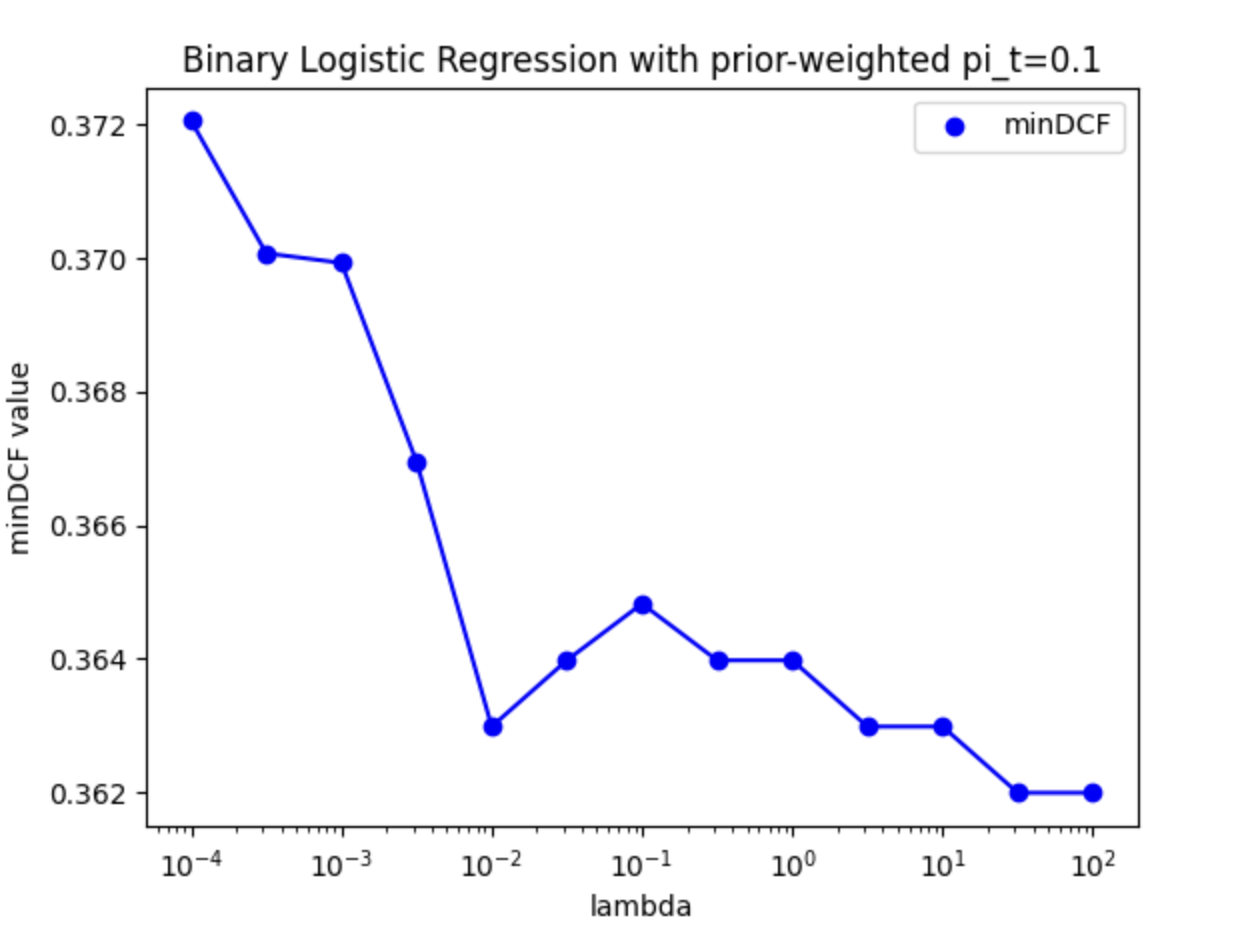
\includegraphics[width=\linewidth]{./img/LLR_W1.png}
            % Rimuovi la caption e l'etichetta da qui
        \end{minipage}%
        \begin{minipage}{.23\textwidth}
            \centering
            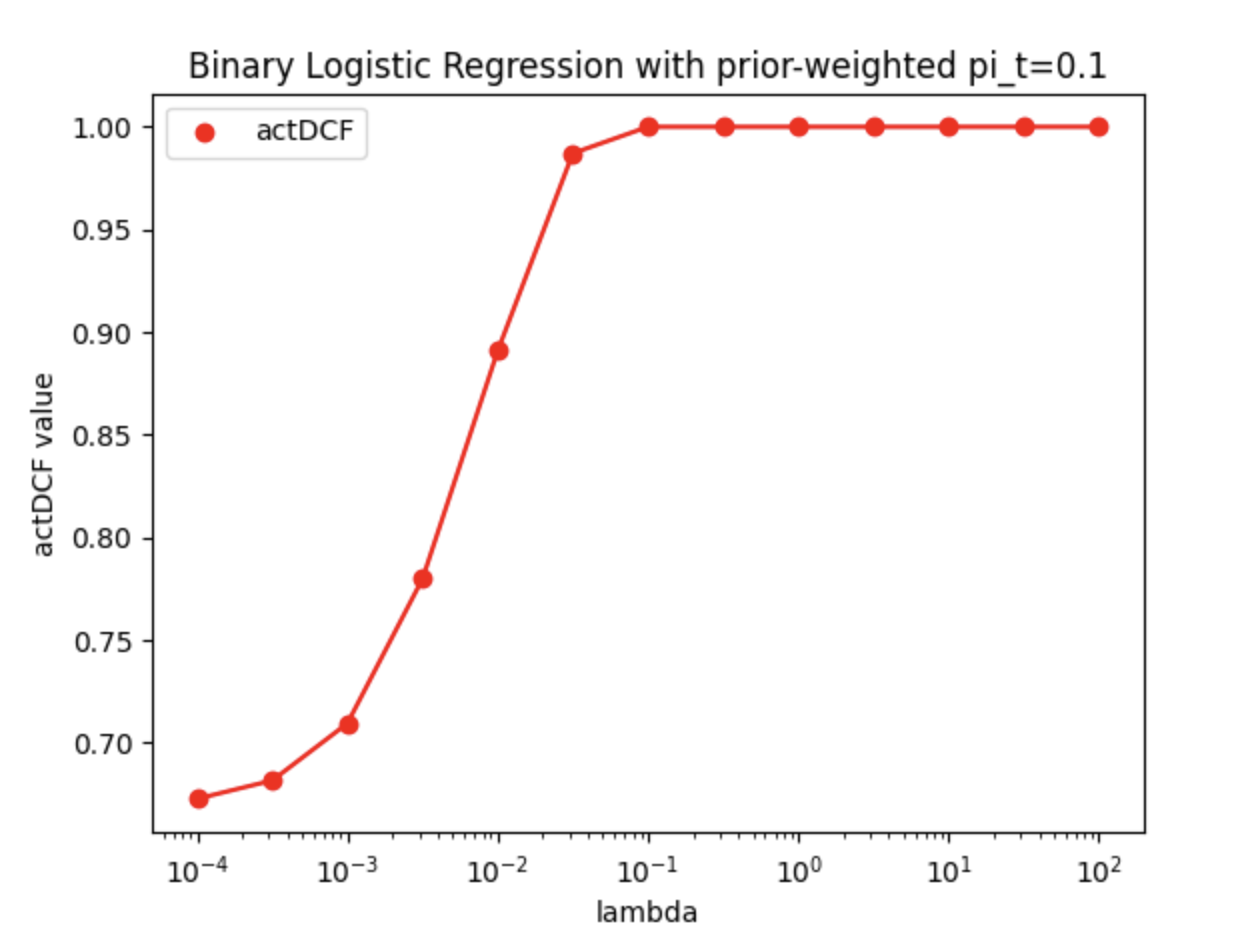
\includegraphics[width=\linewidth]{./img/LLR_W2.png}
            % Rimuovi la caption e l'etichetta da qui
        \end{minipage}
        \begin{minipage}{.23\textwidth}
            \centering
            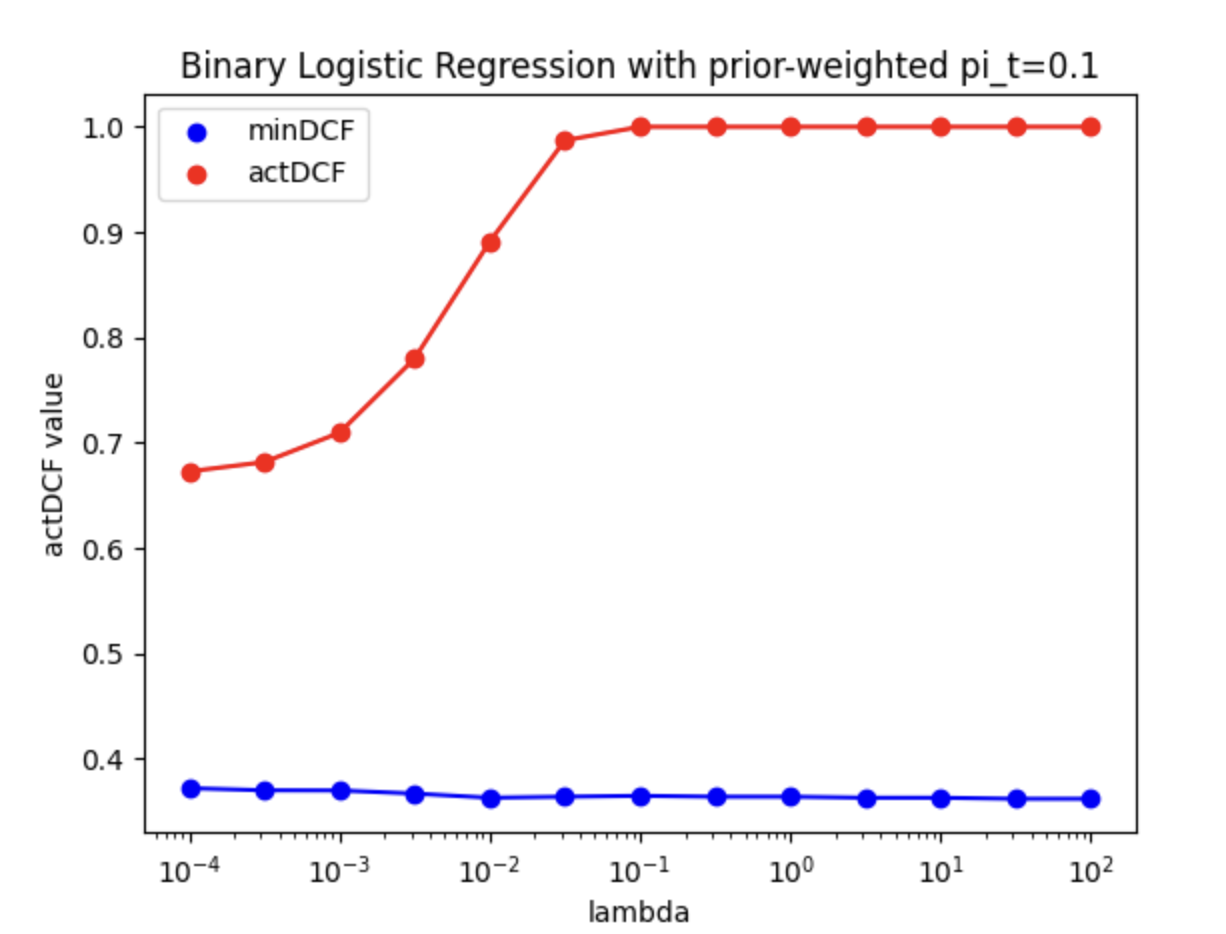
\includegraphics[width=\linewidth]{./img/LLR_W3.png}
            % Rimuovi la caption e l'etichetta da qui
        \end{minipage}
        \begin{minipage}{.23\textwidth}
            \centering
            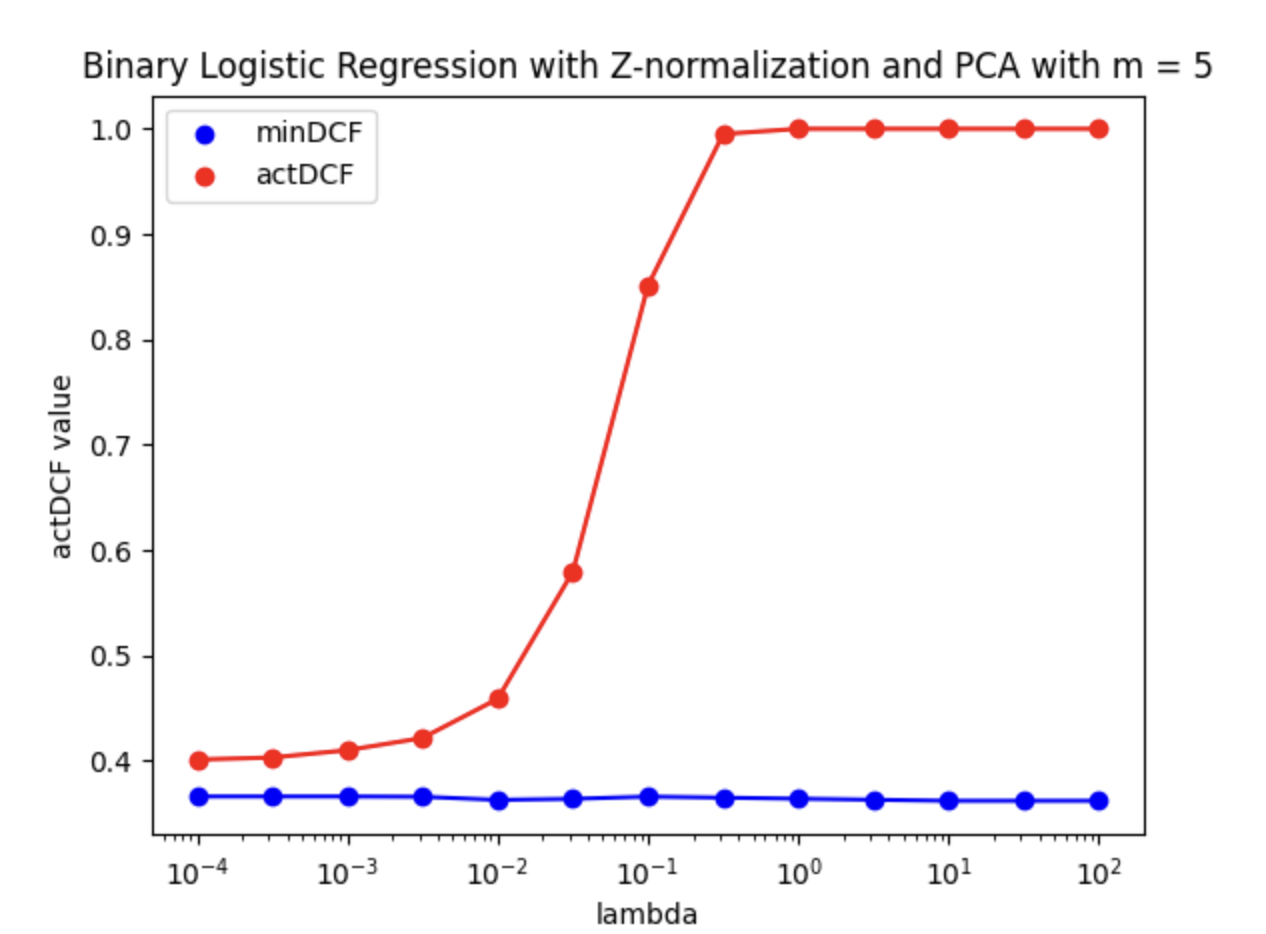
\includegraphics[width=\linewidth]{./img/LLR_Z2.png}
            % Rimuovi la caption e l'etichetta da qui
        \end{minipage}
        \begin{minipage}{.23\textwidth}
            \centering
            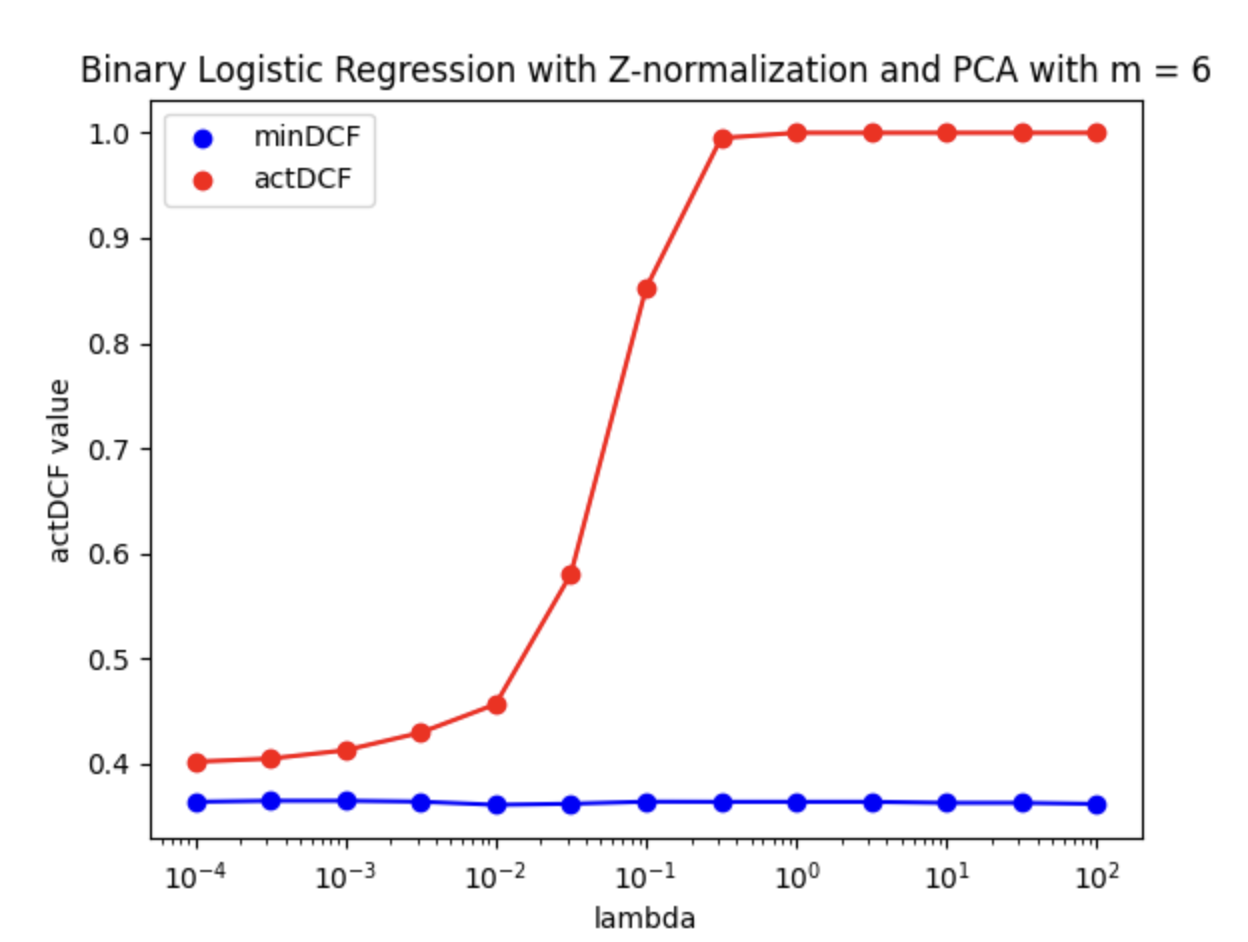
\includegraphics[width=\linewidth]{./img/LLR_Z3.png}
            % Rimuovi la caption e l'etichetta da qui
        \end{minipage}
        \caption{Binary Logistic Regression Model with prior-weighted prior=0.1} % Aggiungi una caption unica qui
        \label{fig:LLR_model_W} % Aggiungi un'etichetta unica qui
    \end{figure}


\begin{itemize}
    \item In logistic regression, prior is a parameter that represents our a priori knowledge about the distribution of labels in the dataset. 
In other words, it is the probability that a random sample belongs to a certain class before we have seen the data.  
So in our current case we use the prior to weight the samples during model training. In particular, samples in the higher priority class receive a higher weight than those in the lower priority class. 
This can be useful if the dataset is unbalanced, the choice of the prior must be made at the beginning and this choice can affect the model a lot, in fact we may even have a worsening of the model. 
\item In our case for example we do not see a significant model worsening, in fact our dataset is not particularly unbalanced, so we can see a significant worsening of the actDCF by applying binary logistic regression with prior-weighted \(\pi_T=0.1\).
\end{itemize}
\subsubsection*{Binary Logistic Regression with Pre-Processing (PCA)}
We can now analyze the results obtained by applying the model after applying PCA, always using \(\pi_T=0.1\)
    \begin{table}[H]
        \centering
        \begin{tabular}{>{\centering\arraybackslash}m{1cm} >{\centering\arraybackslash}m{2cm} >{\centering\arraybackslash}m{2cm} >{\centering\arraybackslash}m{2cm} >{\centering\arraybackslash}m{2cm}}
        \hline
        \multicolumn{5}{c}{\textbf{Binary Logistic Regression with PCA}} \\ \hline
        \textbf{\(\lambda\)} & \multicolumn{2}{c}{\textbf{minDCF}} & \multicolumn{2}{c}{\textbf{actDCF}} \\ \cline{2-5} 
         & \textbf{no z-norm} & \textbf{z-norm} & \textbf{no z-norm} & \textbf{z-norm} \\ \hline
        \multicolumn{5}{c}{m=5}\\  \hline
        \textbf{\(10^{-4}\)} & 0.366103 &  0.366103 & 0.401098 & 0.401097 \\
        \textbf{\(10^{-3}\)} & 0.366103 & 0.366103 & 0.410026 & 0.410026 \\
        \textbf{\(10^{-2}\)} & 0.361847 & 0.362839 & 0.457773 & 0.458765 \\
        \textbf{\(10^{-1}\)} & 0.365959 & 0.365959 & 0.849206 & 0.851190\\ \hline
        \multicolumn{5}{c}{m=6}\\  \hline
        \textbf{\(10^{-4}\)} & 0.363975 & 0.363975 &0.402089 & 0.402089 \\
        \textbf{\(10^{-3}\)} & 0.364967 & 0.364967 & 0.413002 & 0.413002\\
        \textbf{\(10^{-2}\)} & \textcolor{red}{0.361143} & 0.361143 & 0.456781 & 0.456781 \\
        \textbf{\(10^{-1}\)} & 0.364119 & 0.364119 & 0.851190 & 0.852183 \\ \hline
        \end{tabular}
        \caption{minDCF and actDCF}
        \label{tab:LLR_PCA}
    \end{table}
   We can conclude by looking at the table that the application of PCA does not give a significant improvement, as noted earlier, but we can state that performance remains constant.

\subsubsection{Quadratic Logistic Regression}
Now we can analyze training on a Quadratic Logistic Regression model by performing features expansion. We can write log-likelihood ratio as:
\begin{equation}
    \log{\frac{P(C=h_1|x)}{P(C=h_0|x)}}=x^TAx+b^Tx+c=s(\textbf{x},\textbf{A},\textbf{b},\textbf{c})
\end{equation}
This expression is quadratic in x but it's linear in A and b. We could rewrite it to obtain a decision function that is linear for the expanded features space but quadratic in original features space.\\
We can write features expansion as:
\begin{equation}
    \Phi(x)= 
    \begin{bmatrix}
        vec(xx^T) \\
        x
    \end{bmatrix},
    \;\;
    w=
    \begin{bmatrix}
        vec(A) \\
        b
    \end{bmatrix}
\end{equation}
where vec(X) is the operator that stacks the columns of X into a single column vector. In this way we can write the posterio log-likelihood as:
\begin{equation}
    s(x,w,c)=s^T\phi(x)+c
\end{equation}
\begin{figure}[H]
    \centering
    \begin{minipage}{.3\textwidth}
        \centering
        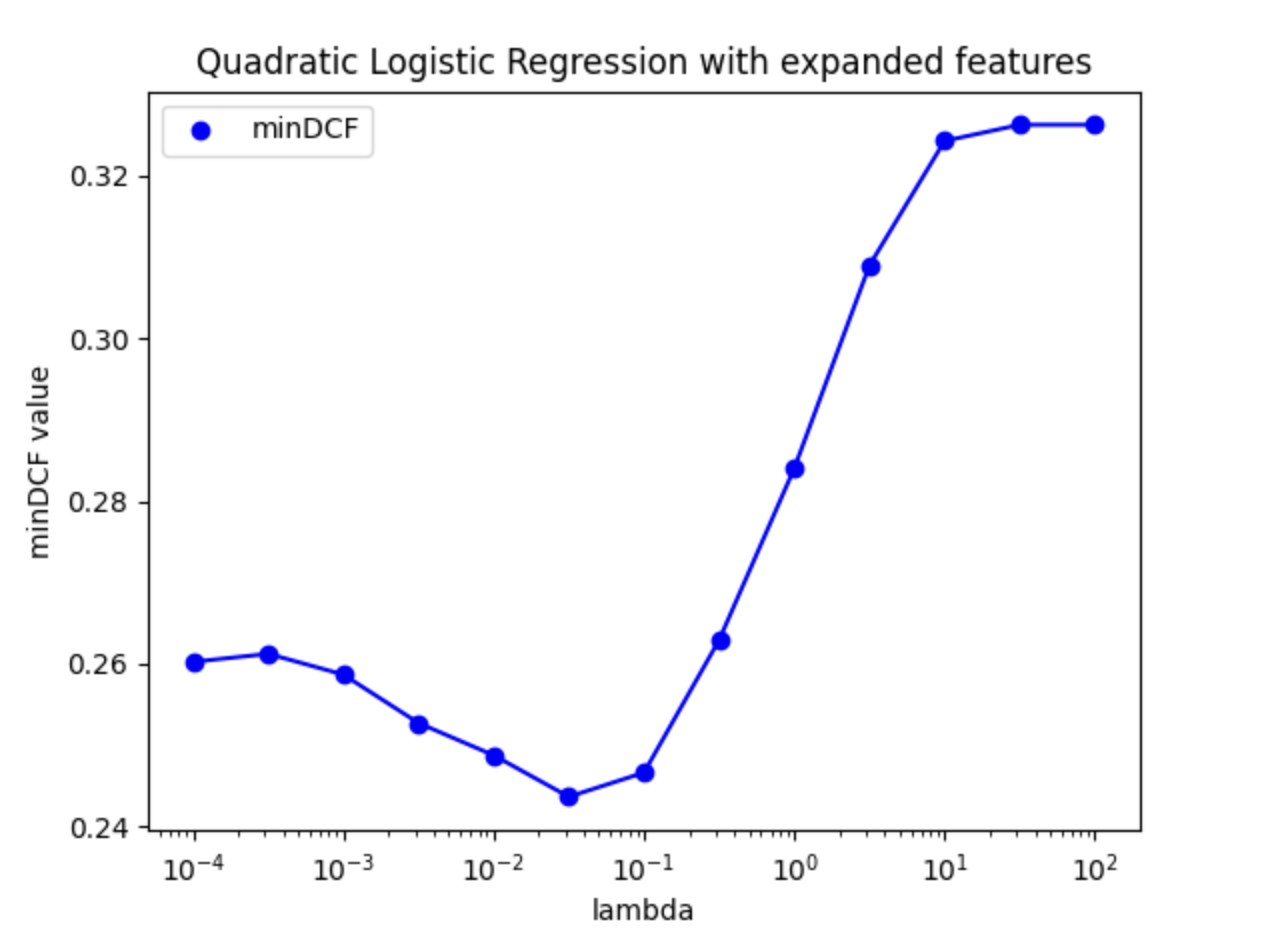
\includegraphics[width=\linewidth]{./img/QLR1.png}
        % Rimuovi la caption e l'etichetta da qui
    \end{minipage}%
    \begin{minipage}{.3\textwidth}
        \centering
        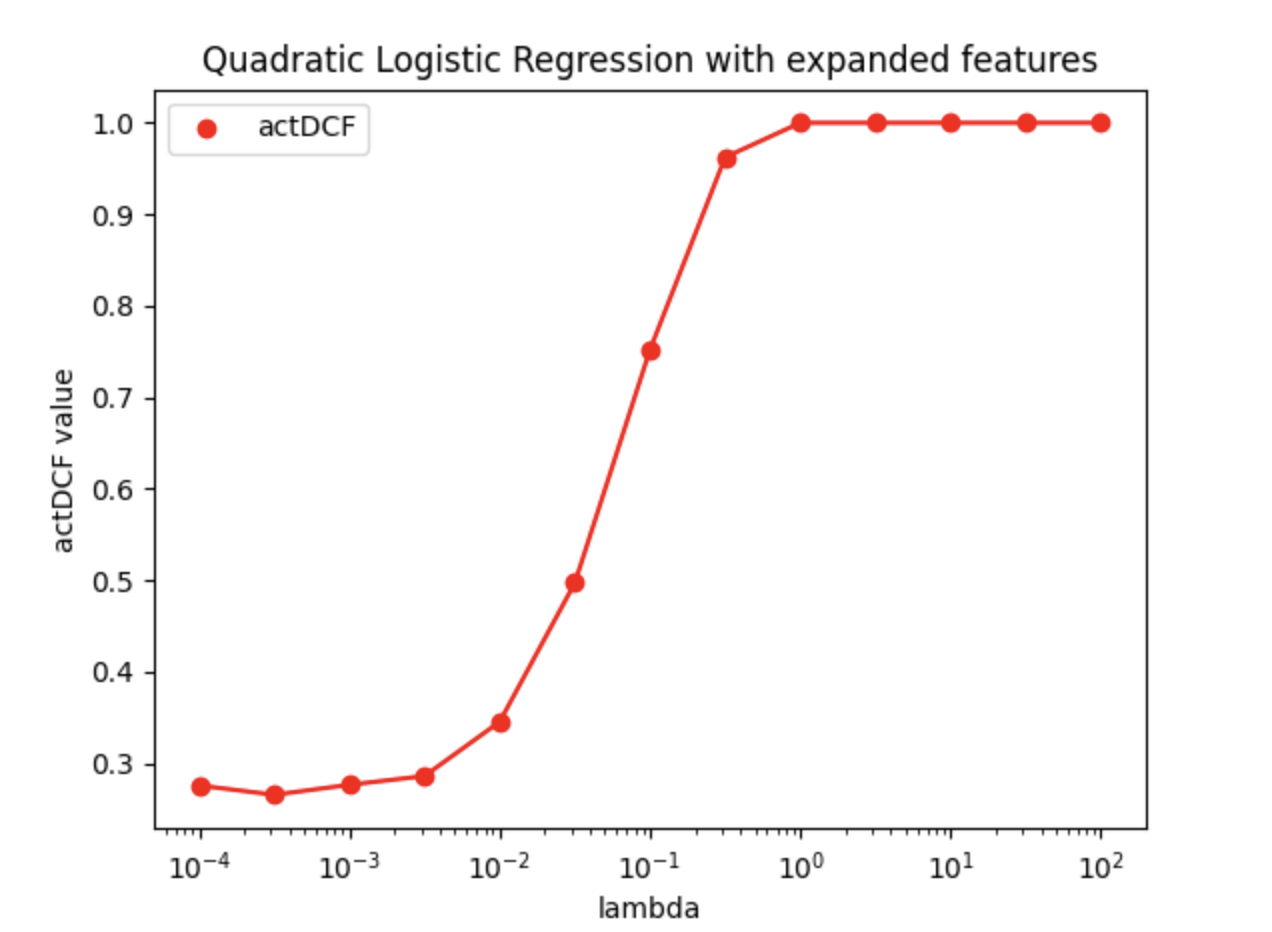
\includegraphics[width=\linewidth]{./img/QLR2.png}
        % Rimuovi la caption e l'etichetta da qui
    \end{minipage}
    \begin{minipage}{.3\textwidth}
        \centering
        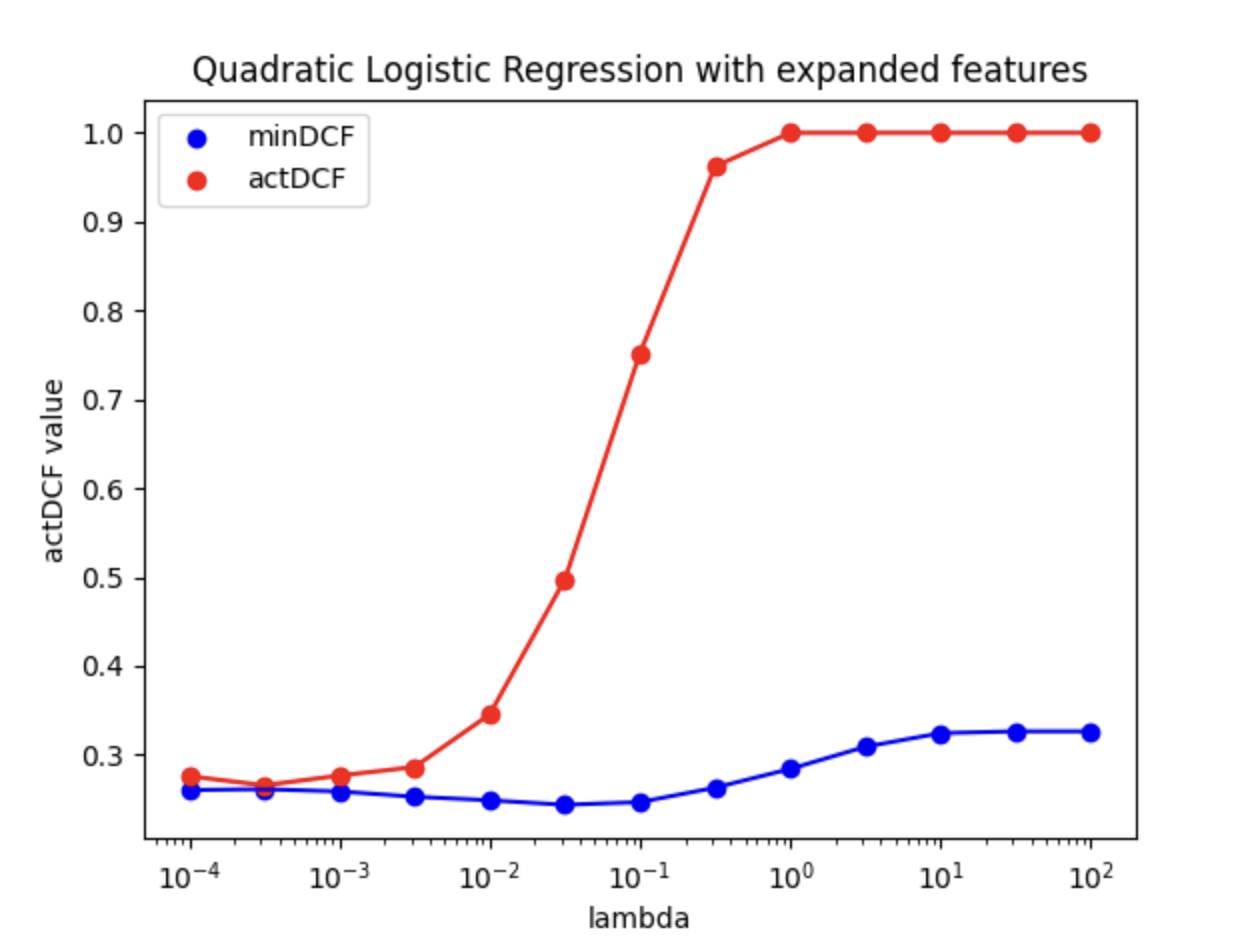
\includegraphics[width=\linewidth]{./img/QLR3.png}
        % Rimuovi la caption e l'etichetta da qui
    \end{minipage}
    \caption{Quadratic Logistic Regression} % Aggiungi una caption unica qui
    \label{fig:QLR_model} % Aggiungi un'etichetta unica qui
\end{figure}
  
\begin{table}[H]
    \centering
    \begin{tabular}{>{\centering\arraybackslash}m{2cm} >{\centering\arraybackslash}m{3cm}>{\centering\arraybackslash}m{2cm}}
    \hline
    \textbf{\(\lambda\)}  &  \textbf{minDCF} & \textbf{actDCF} \\ \hline
    \textbf{\(10^{-4}\)} &  0.260224 & 0.275809 \\
    \textbf{\(10^{-3}\)} & 0.258656 & 0.276514 \\
    \textbf{\(10^{-2}\)} & 0.248736 & 0.345382 \\
    \textbf{\(0.316*10^{-1}\)}&\textcolor{red}{0.243631}&0.497167\\
    \textbf{\(10^{-1}\)} &  0.246607 & 0.751984 \\\hline
    
    \end{tabular}
    \caption{minDCF and actDCF}
    \label{tab:QLR}
    \end{table}

 The quadratic model can help us extract correlations between features that cannot be extracted by a linear model, in our case we can see that Quadratic Logistic Regression performs better than Binary Logistic Regression with and without prior-weighted.

\subsubsection*{Conclusion for Binary Logistic Regression}
\begin{itemize}
    \item We can see that applying z-normalization does not bring us significant changes in the observed metrics, it could be because of the invariance of Logistic Regression in fact being based on a linear function of the data, it is invariant to linear transformations of the data, i.e. it does not change the ability of the model to separate classes if the relationship between the features and the label is already linearly separable.  Also if the regularization parameter is chosen appropriately this could minimize the effect of z-normalization. Finally, if our data are already distributed such that features contribute equally to the model decision, z-normalization may not have a significant impact.  
    \item For all the various models represented in
    Figure ~\ref{fig:LLR_model} ,
    Figure ~\ref{fig:LLR_model_W} ,
    Figure ~\ref{fig:QLR_model} ,
    it can be seen that \(\lambda\) significantly affects actDCF and minDCF. In fact, it can be seen that for values greater than \(10^{-1}\) there is significant degradation. It is necessary to remember that a larger value of \(\lambda\) may lead to overgeneralization which may lead to underfitting, while for too small values of it there may be low generalization and thus there may be overfitting. Based on this analysis, large values of \(\lambda\) were excluded in the tables showing the different values of minDCF and actDCF for lambda ranging from \(10^{-4}\) to \(10^{-1}\).
\item After doing various analyses we can see which are the optimal values of lambda as mentioned above 
and which model gives the best performance comparing for now the minDCF, also the difference we can see between minDCF and actDCF suggests i that the models do not have a good calibration.
In our case quadratic logistic regression seems to give the best results, so we can draw that we need the model to be able to capture nonlinear relationships between variables and thus be able to find nonlinear separations rules in the feature space.
\item From the results we can observe that in fact we get better results with a relatively higher lambda so we can conclude that we need more regularization to prevent overfitting.
\end{itemize}
\underline{Best Logistic Regression Model} analyzed for our main application that is application with \(\pi_T=0.1\) is:
\begin{itemize}
    \item \textbf{Quadratic Logistic Regression} with \(\lambda=0.0316228\), no prior-weighted
\end{itemize}

\subsection{SVM Classifier}
\subsubsection{Linear SVM}
Support Vector Machines are linear classifiers that look for maximum margin separation hyperplanes.
\\The primal formulation of the soft-margin SVM problem consists in minimizing the function:
\begin{equation}
    \mathbf{J}(w,b)= \frac{1}{2}||w||^2 + C\sum_{i=1}^{N}max(0,1-z_i(w^Tx_i+b))
\end{equation}
where N is the number of training samples, C is the regularization parameter, and \(z_i\) is the margin of the i-th sample.\\
The dual formulation of the problem is:
\begin{equation}
    \mathbf{J}(\alpha)= - \frac{1}{2} \alpha^T \;\textbf{H} \;\alpha + \alpha^T \textbf{1} \;\;\;\;\;\;1\leq \alpha_i\leq C,\;\; \forall i \in \{1,...,N\},\;\; \sum_{i=1}^{n}\alpha_i z_i=0
\end{equation}
where H is \(H_{ij}=z_iz_jx_i^Tx_j\) and the dual solution is the maximizer of \(J^D(\alpha)\).\\
Primal and dual solutions are releted through:
\begin{equation}
    w^*=\sum_{i=1}^{N}\alpha_i^* z_i x_i
\end{equation}
In addition it's possible to rewrite dual problem as minimization of:
\begin{equation}
   \hat{\mathbf{L}}(\alpha)=-\mathbf{J}(\alpha)= \frac{1}{2} \alpha^T \;\textbf{H} \;\alpha - \alpha^T \textbf{1}
\end{equation}
and it can be minimize by L-BFGS-B algorithm.
After that we have calculated the optimal \(\alpha\) we can compute \(w^*\).
\begin{figure}[H]
    \centering
    \begin{minipage}{.3\textwidth}
        \centering
        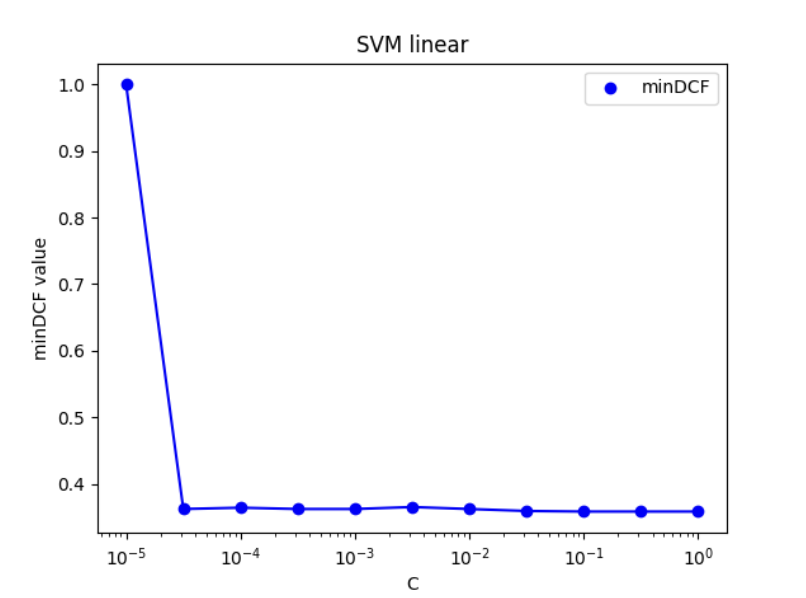
\includegraphics[width=\linewidth]{./img/SVM_L1.png}
        % Rimuovi la caption e l'etichetta da qui
    \end{minipage}%
    \begin{minipage}{.3\textwidth}
        \centering
        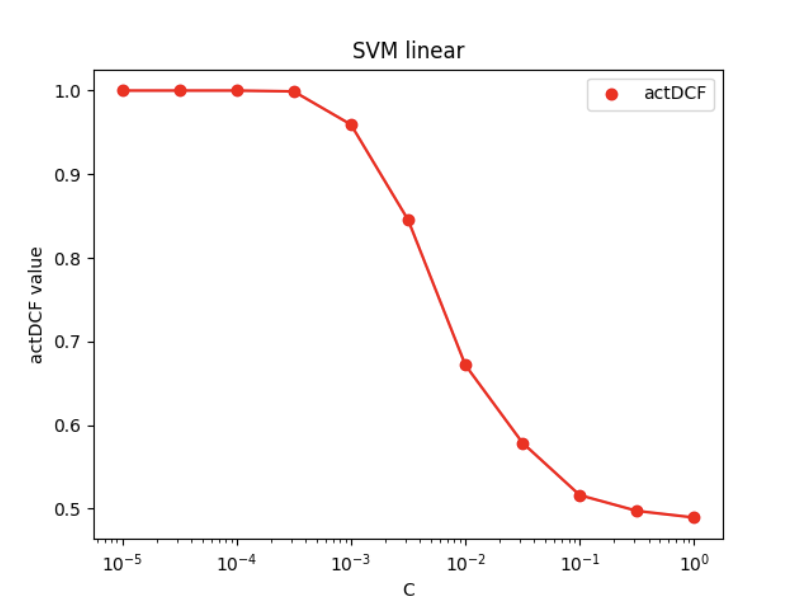
\includegraphics[width=\linewidth]{./img/SVM_L2.png}
        % Rimuovi la caption e l'etichetta da qui
    \end{minipage}
    \begin{minipage}{.3\textwidth}
        \centering
        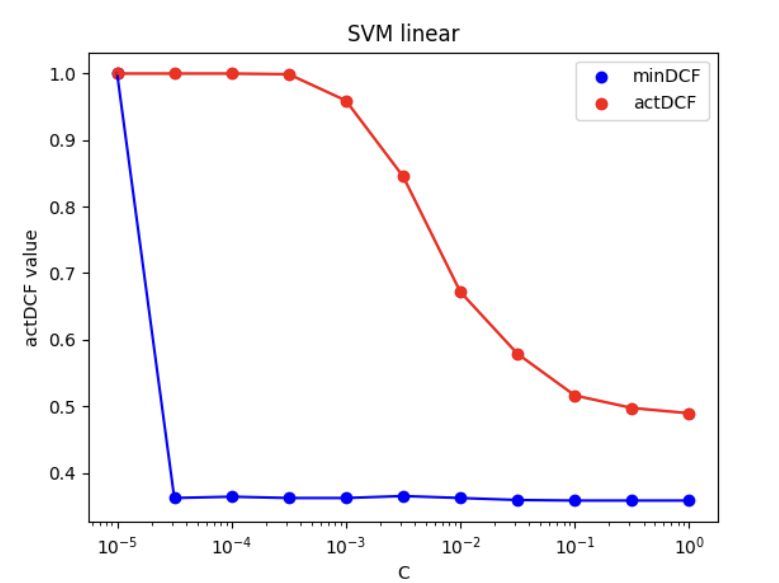
\includegraphics[width=\linewidth]{./img/SVM_L3.png}
        % Rimuovi la caption e l'etichetta da qui
    \end{minipage}
    \caption{SVM} % Aggiungi una caption unica qui
    \label{fig:SVM} % Aggiungi un'etichetta unica qui
\end{figure}
\begin{table}[H]
    \centering
    % \begin{tabular}{>{\centering\arraybackslash}m{2cm} >{\centering\arraybackslash}m{3cm}>{\centering\arraybackslash}m{2cm}}
    % \hline
    % \multicolumn{3}{c}{\textbf{Linear SVM with K=1.0}} \\   \hline
    % \textbf{C}  &  \textbf{minDCF} & \textbf{actDCF} \\ \hline
    \begin{tabular}{>{\centering\arraybackslash}m{1cm} >{\centering\arraybackslash}m{2cm} >{\centering\arraybackslash}m{2cm} >{\centering\arraybackslash}m{2cm} >{\centering\arraybackslash}m{2cm}}
    \hline
    \multicolumn{5}{c}{\textbf{Linear SVM with K=1.0}} \\ \hline
    \textbf{C} & \multicolumn{2}{c}{\textbf{minDCF}} & \multicolumn{2}{c}{\textbf{actDCF}} \\ \cline{2-5} 
     & \textbf{no z-norm} & \textbf{z-norm} & \textbf{no z-norm} & \textbf{z-norm} \\ \hline
    \textbf{\(10^{-5}\)} & 1.0 & 1.0 & 1.0 & 1.0 \\
    \textbf{\(10^{-4}\)} & 0.363975& 0.363975 & 1.0 & 1.0 \\
    \textbf{\(10^{-3}\)} & 0.361991& 0.361991 & 0.959325 & 0.959325\\
    \textbf{\(10^{-2}\)} & 0.361991& 0.361991 & 0.671770 & 0.671770\\
    \textbf{\(10^{-1}\)} & 0.358167& 0.358166 & 0.516161& 0.516161\\
    \textbf{\(10^{0}\)}  & 0.358167& 0.358167 & 0.489375& 0.489375\\\hline
    \end{tabular}
    \caption{minDCF and actDCF}
    \label{tab:SVM_linear}
    \end{table}
\subsubsection{Kernel SVM}
SVMs allow nonlinear classification through the kernel trick. 
Unlike the quadratic logistic regression classifier, there is no explicit expansion of the feature space; 
we only need to be able to calculate the scalar product between the expanded features:\( k(x_1,x_2)=\phi(x_1)_T\phi(x_2)\) where k is the kernel function.
To do this we need to go and replace H with \(\hat{H}= z_iz_jk(x_1,x_2)\). 
We can observe two different types of kernels:
\begin{itemize}
    \item \textbf{Polynomial kernel of degree d}: \(k(x_1,x_2)=(x_1^Tx_2+c)^d\)
    \item \textbf{Radial Basis Function kernel(RBF)}: \(k(x_1,x_2)=e^{-\gamma||x1-x_2||^2}\)
\end{itemize}
We can now apply the polynomial kernel to the SVM with \(d=2,\;\; c=1, \;\;\xi=0\) and see how minDCF and actDCF vary as C changes.
\begin{figure}[H]
    \centering
    \begin{minipage}{.3\textwidth}
        \centering
        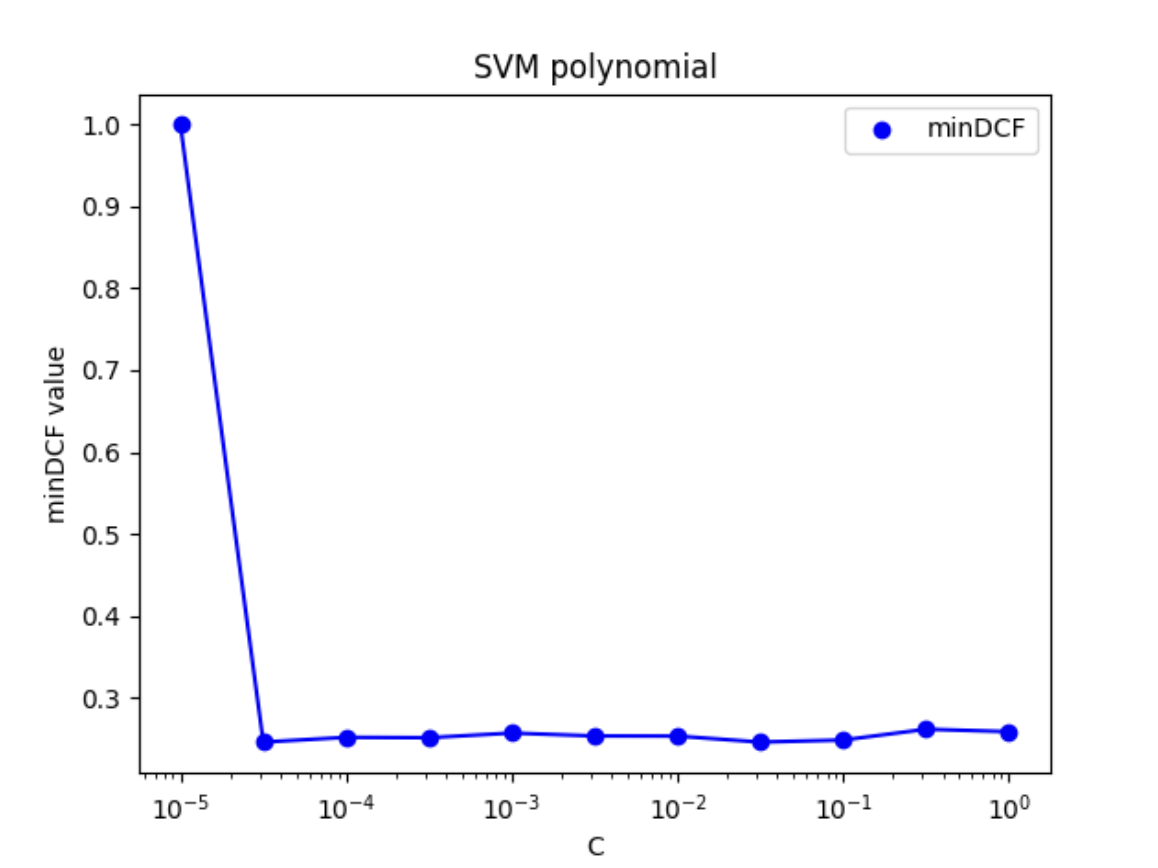
\includegraphics[width=\linewidth]{./img/SVM_P1.png}
        % Rimuovi la caption e l'etichetta da qui
    \end{minipage}%
    \begin{minipage}{.3\textwidth}
        \centering
        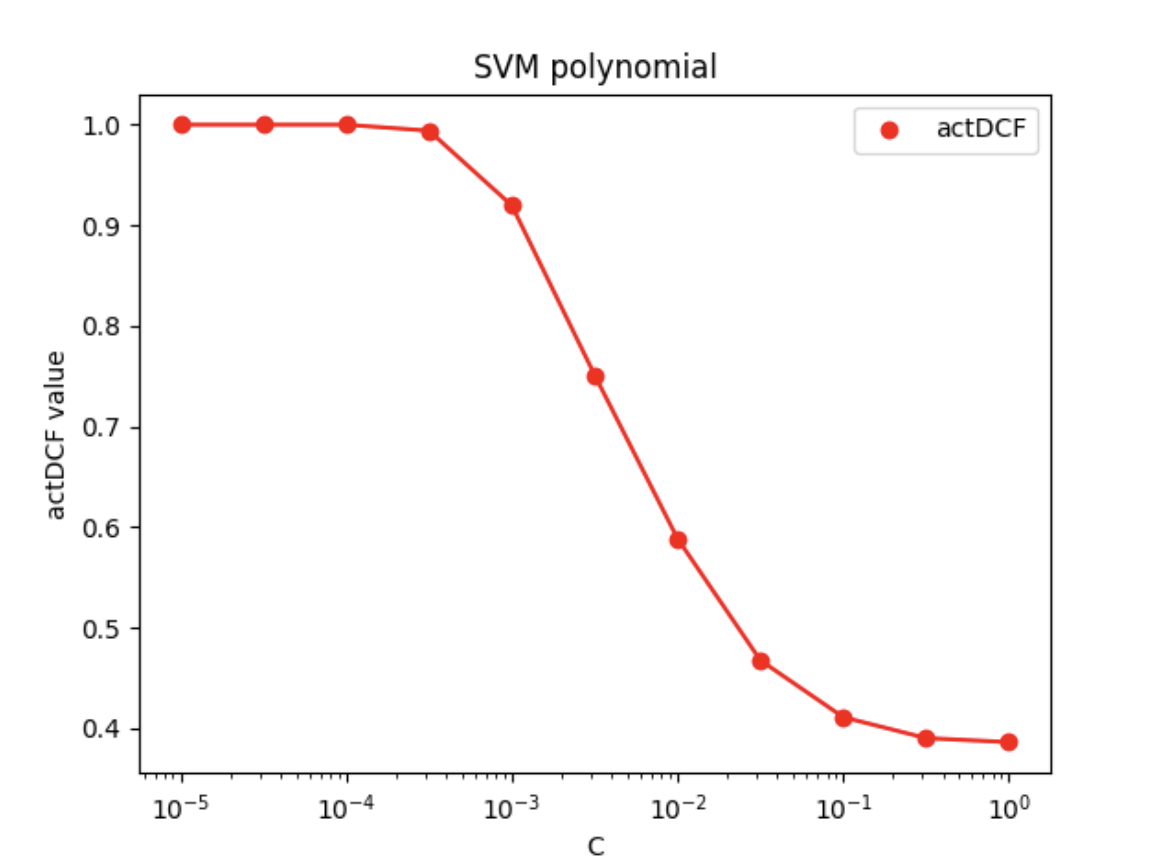
\includegraphics[width=\linewidth]{./img/SVM_P2.png}
        % Rimuovi la caption e l'etichetta da qui
    \end{minipage}
    \begin{minipage}{.3\textwidth}
        \centering
        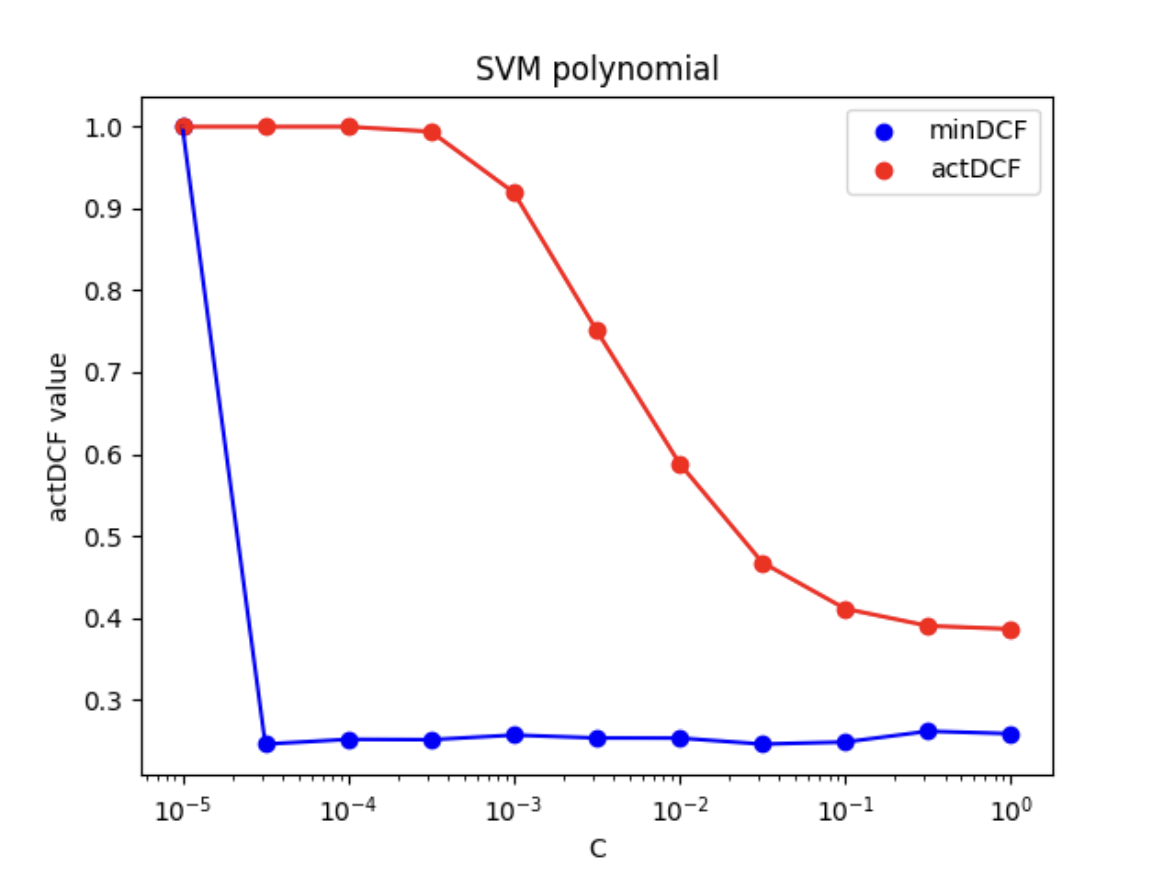
\includegraphics[width=\linewidth]{./img/SVM_P3.png}
        % Rimuovi la caption e l'etichetta da qui
    \end{minipage}
    \caption{SVM with Polynomial kernel} % Aggiungi una caption unica qui
    \label{fig:SVM_p} % Aggiungi un'etichetta unica qui
\end{figure}
\begin{table}[H]
    \centering
    \begin{tabular}{>{\centering\arraybackslash}m{2cm} >{\centering\arraybackslash}m{3cm}>{\centering\arraybackslash}m{2cm}}
    \hline
    \multicolumn{3}{c}{\textbf{Polynomial kernel SVM ~ \(d=2,\;\; c=1, \;\;\xi=0\) }} \\   \hline
    \textbf{C}  &  \textbf{minDCF} & \textbf{actDCF} \\ \hline
    \textbf{\(10^{-4}\)} & 0.251296 & 1.0\\
    \textbf{\(10^{-3}\)} & 0.256544 & 0.9196428\\
    \textbf{\(10^{-2}\)} & 0.252848 & 0.588437 \\
    \textbf{\(10^{-1}\)} & 0.248031 & 0.410858\\
    \textbf{\(10^{0}\)} &  0.258240 & 0.386056\\
    \textbf{\(10^{1}\)} & 0.269297 & 0.380104\\
    \textbf{\(10^{2}\)} & 0.261920 & 0.342837\\
    \hline
    \end{tabular}
    \caption{minDCF and actDCF}
    \label{tab:SVM_Poly}
    \end{table}
    In this case instead we apply to SVM the RBF kernel with \(\xi=1\) and yet in a first analysis as we can see from Figure~\Ref{fig:SVM_RBF} , we make an analysis of how minDCF and actDCF vary as \(\gamma\) varies. From this analysis we can derive that the best value for it is 0.1.
    \begin{figure}[H]
        \centering
        \begin{minipage}{.4\textwidth}
            \centering
            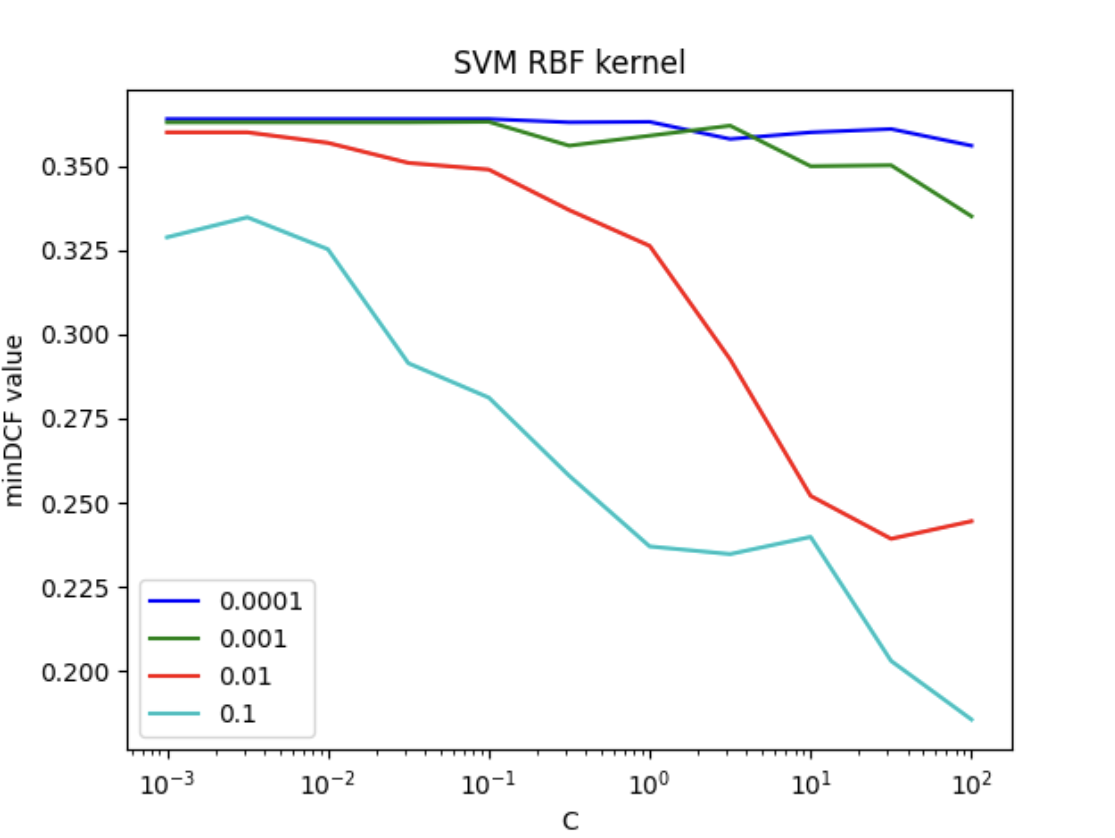
\includegraphics[width=\linewidth]{./img/SVM_RBF1.png}
            % Rimuovi la caption e l'etichetta da qui
        \end{minipage}%
        \begin{minipage}{.4\textwidth}
            \centering
            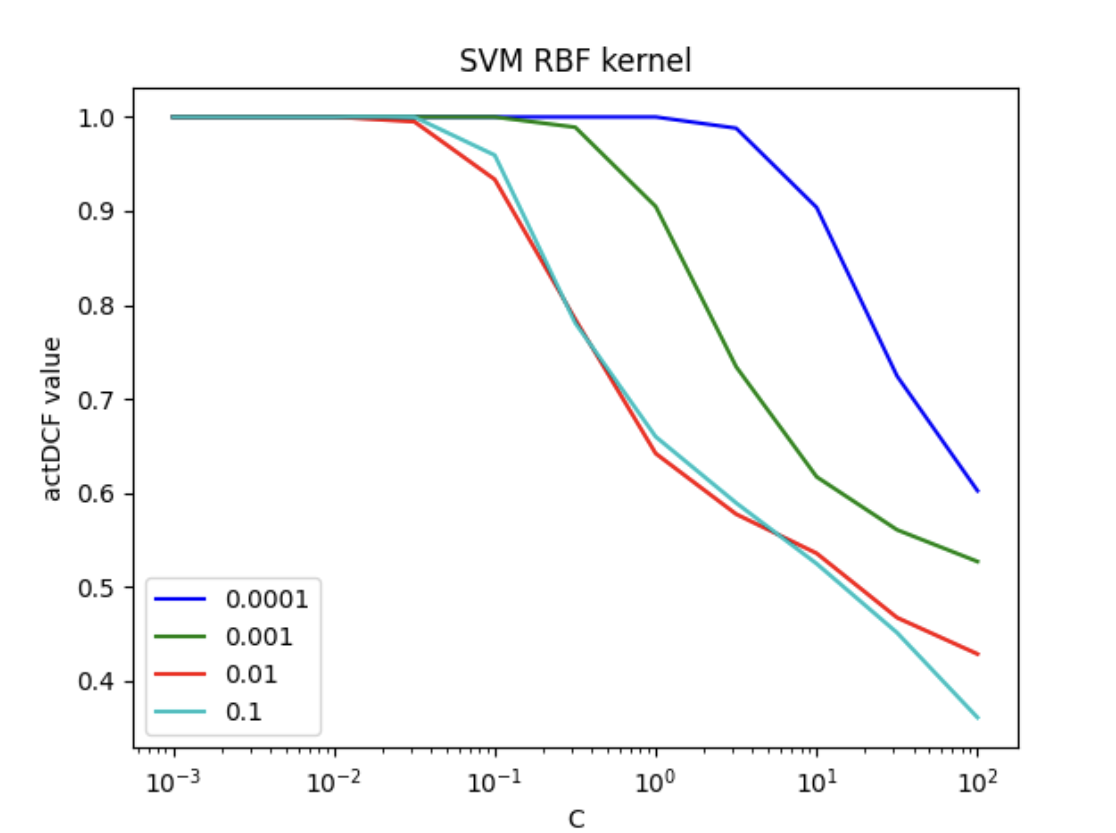
\includegraphics[width=\linewidth]{./img/SVM_RBF2.png}
            % Rimuovi la caption e l'etichetta da qui
        \end{minipage}
        \caption{SVM with RBF kernel} % Aggiungi una caption unica qui
        \label{fig:SVM_RBF} % Aggiungi un'etichetta unica qui
    \end{figure}


    \begin{figure}[ht]
        \begin{minipage}[b]{0.5\textwidth}
            \centering
        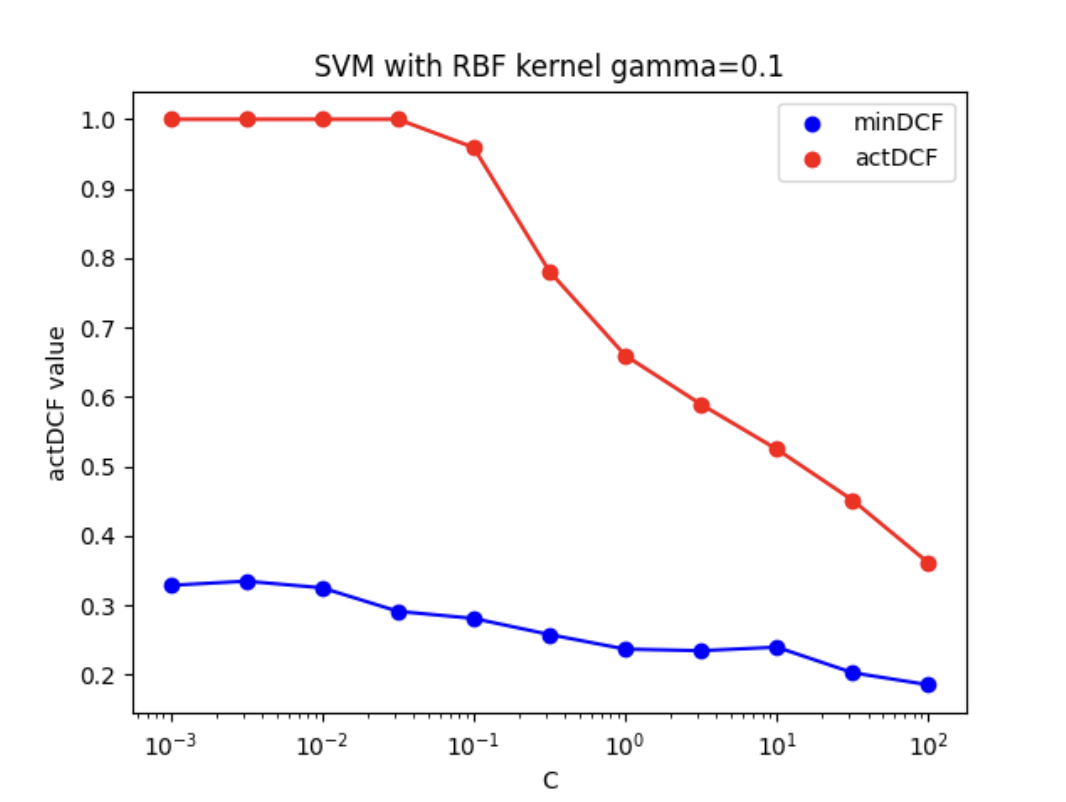
\includegraphics[width=0.7\textwidth]{./img/SVM_RBF3.png}
        \caption{Variance of data for each m values}
        \label{fig:SVM_RFD3}
        \end{minipage}
        \hfill % Aggiunge uno spazio orizzontale tra le due minipage se necessario
        \begin{minipage}[b]{0.5\textwidth}
        \centering
    \begin{tabular}{>{\centering\arraybackslash}m{2cm} >{\centering\arraybackslash}m{3cm}>{\centering\arraybackslash}m{2cm}}
    \hline
    \multicolumn{3}{c}{\textbf{RBF kernel SVM ~ \(\xi=1 \;\;\gamma=0.1\) }} \\   \hline
    \textbf{C}  &  \textbf{minDCF} & \textbf{actDCF} \\ \hline
    \textbf{\(10^{-3}\)} & 0.328821 & 1.0\\
    \textbf{\(10^{-2}\)} & 0.325284 & 1.0 \\
    \textbf{\(10^{-1}\)} & 0.281201 & 0.959325\\
    \textbf{\(10^{0}\)} & 0.236975 & 0.659866\\
    \textbf{\(10^{1}\)} & 0.239807 & 0.524801\\
    \textbf{\(10^{2}\)} & \textcolor{red}{0.185531} & 0.361111\\
    \hline
    \end{tabular}
    \caption{minDCF and actDCF}
    \label{tab:SVM_RDF}
    \end{minipage}
    \end{figure}
\subsubsection*{Conclusion for SVM}
\begin{itemize}
    \item Again as in logistic regression, we do not see any substantial changes in performance even after applying z-normalization.
    \item We can also draw conclusions by seeing the performance of the metrics when we vary the parameter C, in fact lower values of C imply strong regularization while low values imply weak regularization. We can see that for higher values of C we will have better calibration since the value of actDCF also decreases, while minDCF remains quite low and stable for all tested values of C.
    \item \textbf{SVM with Polynomial kernel:}
    \begin{itemize}
    \item When we apply SVM with polynomial kernel we can see that the results are lower than those of linear SVM. We can compare the results obtained to those of the previously analyzed models and we can get that the results obtained are comparable to those obtained with QLR this continues to suggest that there is no linear relationship between the features and therefore we need to model quadratic relationships between the features.
    \item It is also possible to see that in this case compared to previous models the actDCF turns out to be lower so there is a better calibration of the model.
   \end{itemize}
   \item \textbf{SVM with RBF kernel:}
    \begin{itemize}
    \item The best results in this case are obtained with gamma=0.1 as mentioned earlier and with high C so with lower regularization. The calibration in this case is better than in the other models but still turns out to be not well calibrated.
    \item This model also turns out to be the one for which we get better performance so it can be assumed from this that the dataset benefits from nonlinear mapping and that there are complex relationships between features that can be better captured in a higher dimensional space.
   \end{itemize}
\end{itemize}

\underline{Best SVM model} analyzed for our main application that is application with \(\pi_T=0.1\) is:
\begin{itemize}
    \item \textbf{SVM with RBF kernel } with \(\gamma=0.1\;\; K=1\;\; C=10^2\)
\end{itemize}

\subsection{GMM Classifier}
The last model we are going to consider is a generative model. The GMM problem is related to the
estimation of a population distribution and can be also applied to the classification task.
The GMM density consists of a weighted sum of K Gaussians:
\begin{equation}
\mathbf{X}\thicksim  GMM(\mathbf{M} ,\mathcal{S},w)\implies f_x(x)=\sum_{c=1}^{K}\mathcal{N}(x|\mu_g,\Sigma_g)w_g
\end{equation}
where \( M=[\mu_1...\mu_k]\), \(\mathcal{S}=[\Sigma_1...\Sigma_k]\) and \(w=[w_1...w_k]\) are the parameters of the model.\\
Gaussian components can be viewed as clusters to which the samples belong ( hard or soft), and the cluster label is an unobserved latent random variable. We can also introduce a term called responsability that represents the posterior probability that a sample belongs to a certain cluster:
\begin{equation}
    \gamma(z_{n,i})=P(G_i=g| X_i=x)=\frac{f_{x_i,G_i}(x_i,g)}{f_{x_i}(x_i)}=\frac{\mathcal{N}(x_i|\mu_g,\Sigma_g)w_g}{\sum_{g'}\mathcal{N}(x_i|\mu_{g'},\Sigma_{g'})w_{g'}}
\end{equation}
Then assign the sample to the cluster label for which the liability is highest and re-estimate the model parameters based on the cluster assignment. An obvious problem is the creation of hard clusters that do not allow a sample to belong to more than one cluster. To handle soft clusters, scores can be estimated from which we can then obtain new parameters:
In this way we can apply the Expectation-Maximization algorithm:
\begin{itemize}
    \item Expectation stage: estimation of the liability (given the model parameters \((M_t,S_t,w_t)\))
    \item Maximization step: estimation of new model parameters using the above statistics, estimation continues from an initial value of the model parameters until a certain criterion is met. 
\end{itemize}

The EM algorithm then requires an initial estimate for the GMM parameters, so we use the LBG algorithm to incrementally construct a GMM with 2G components from a GMM with G components. The starting point will be \( (1,\mu,\sigma)\), so we use the empirical mean and covariance matrix of the data set. Then it builds a 2-component model starting from one and from each of the new components 2 more components are generated and so on.
GMM can have differents versions as:
\begin{itemize}
    \item \textbf{The diagonal covariance model:} in this setup, the covariance matrix of each component is assumed to be diagonal, which means the variables are considered independent.
    \item \textbf{The full covariance model:} in this case each component has a full covariance matrix, which means that all possible covariances between the variables are considered.
\end{itemize}
It can be assumed that the model with the diagonal covariance can give good results, as the features do not appear to be particularly correlated, however below we go on to analyze the results obtained for the different models.
\\
Through these histograms in Figure~\Ref{fig:GMM_hist} we can see how minDCF changes as the number of components varies and thus which components are worth considering when evaluating GMM
\begin{figure}[H]
    \centering
    \begin{minipage}{.3\textwidth}
        \centering
        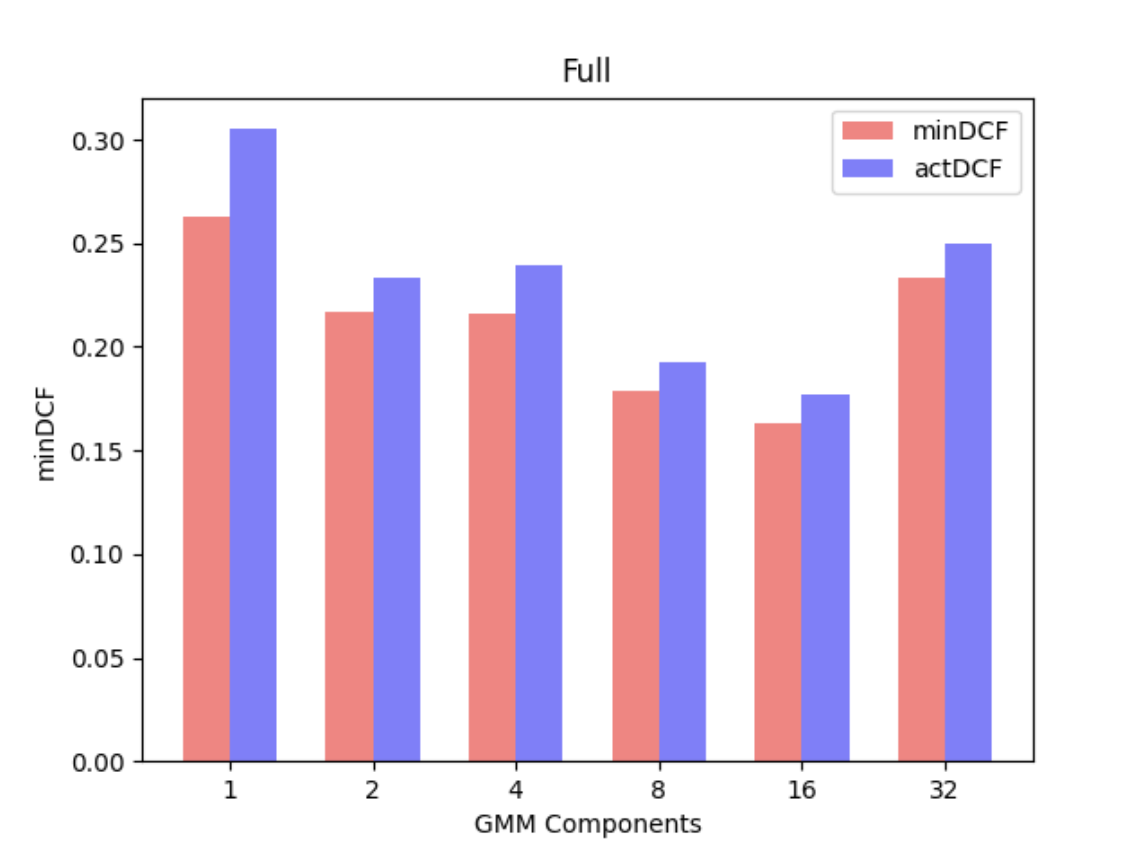
\includegraphics[width=\linewidth]{./img/GMM_Full.png}    
    \end{minipage}%
    \begin{minipage}{.3\textwidth}
        \centering
        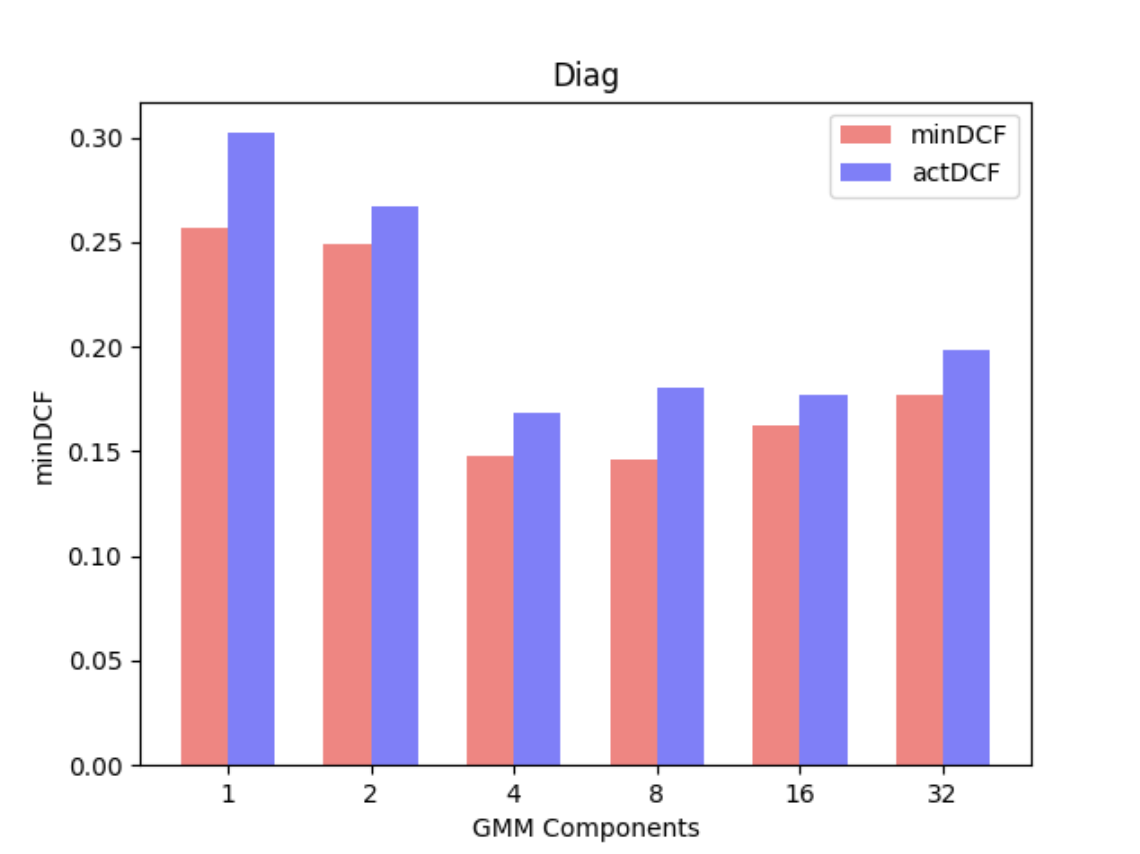
\includegraphics[width=\linewidth]{./img/GMM_diag.png}
    \end{minipage}
    \caption{GMM with diagonal and full covariance matrix} % Aggiungi una caption unica qui
    \label{fig:GMM_hist} 
\end{figure}
During training with the GMM model, all achievable results were tested by giving a different number of components for each class. All possible combinations of the range of number of components chosen was tested both using full Covariance and diag Covariance, it could be concluded that using too low or too high number of components there was a deterioration of the metrics considered.\\
In the Figure~\Ref{fig:GMM_hist} above for class 0 and class 1 the same number of components was used but it is also possible in some cases to optimize the number of components for each class can lead to better discrimination between classes and better classification performance, in this way it is possible to adapt to the specific class.\\
During training with the GMM model, all achievable results were tested by giving precisely a different number of components for each class. All possible combinations of the range of number of components chosen was tested both using full Covariance and diag Covariance, it could be concluded that using too low or too high number of components there was a deterioration of the metrics considered.
\begin{table}[H]
    \centering
    \begin{tabular}{>{\centering\arraybackslash}m{2cm} >{\centering\arraybackslash}m{3cm}>{\centering\arraybackslash}m{2cm}}
    \hline
    \multicolumn{3}{c}{\textbf{GMM model }} \\   \hline
    \textbf{(nc0,nc1)}  &  \textbf{minDCF} & \textbf{actDCF} \\ \hline
    \multicolumn{3}{c}{\textbf{Full cov }} \\   \hline
    \textbf{\((4,16)\)} & 0.174475 & 0.187084\\
    \textbf{\((8,8)\)} & 0.178603 & 0.192764\\
    \textbf{\((8,16)\)} & 0.152649 & 0.172491 \\
    \textbf{\((8,32)\)} & 0.174475 & 0.190348\\
    \textbf{\((16,16)\)} & 0.163130 & 0.176603 \\\hline\hline
    \textbf{\((4,16)\)} & 0.137192 & 0.168666\\
    \textbf{\((8,8)\)} &  0.146265 & 0.180859\\
    \textbf{\((8,16)\)} & 0.132376 & 0.148681\\
    \textbf{\((8,32)\)} & \textcolor{red}{0.131240} & 0.151657 \\
    \textbf{\((16,16)\)} & 0.162154 & 0.176891 \\\hline\hline
    \hline
    \end{tabular}
    \caption{minDCF and actDCF}
    \label{tab:GMM}
    \end{table}
    Only the combinations of number of components for the different classes that appeared to be most promising and representative were given in the Table~\ref{tab:GMM}; the others results can be found in the project code.
\subsubsection*{Conclusion for GMM}
\begin{itemize}
    \item  After applying the model we can conclude that the best performance is achieved by using 8 components for class 0 and 32 components for class 1, the choice of 8 components for class 0 and 32 for class 1 suggests that class 1 requires a more complex model to avoid underfitting, while for class 0 a less complex model is sufficient.\\
    While the better performance using a diagonal type covariance matrix indicates that assuming independence of features from each other leads to better results. This may suggest that the features in the dataset have a primarily independent relationship and that the additional complexity introduced by a full covariance matrix does not provide significant benefits in terms of model performance.
    \item Compared with the other models, it is also possible to see that the results are better calibrated than all the other cases, in fact, in addition to being the model that gives us lower minDCF than all the others, it is also the one that is better calibrated.
\end{itemize}
\underline{Best GMM model} analyzed for our main application that is application with \(\pi_T=0.1\) is:
\begin{itemize}
    \item \textbf{GMM with diag covariance} with \(nComponents=8\) for class 0 and \(nComponents=32\) for class 1.
\end{itemize}
\section{Score Calibration}
\subsection{Calibration Analysis on Selected Models}
\subsection*{Best models}
\begin{itemize}
    \item \textbf{Logistic Regression:} QLR with \(\lambda=0.03162277660168379\), Best minDCF: 0.243631592421915
    \item \textbf{SVM:} SVM with RBF kernel \(C=10^2\;\; \gamma=0.1\), Best minDCF  0.18553187403993854
    \item \textbf{GMM:} GMM with Diag covariance \(nComponents=8\) for class 0 and \(nComponents=32\) for class 1, Best minDCF 0.131240
\end{itemize}
\begin{figure}[H]
    \centering
    \begin{minipage}{.3\textwidth}
        \centering
        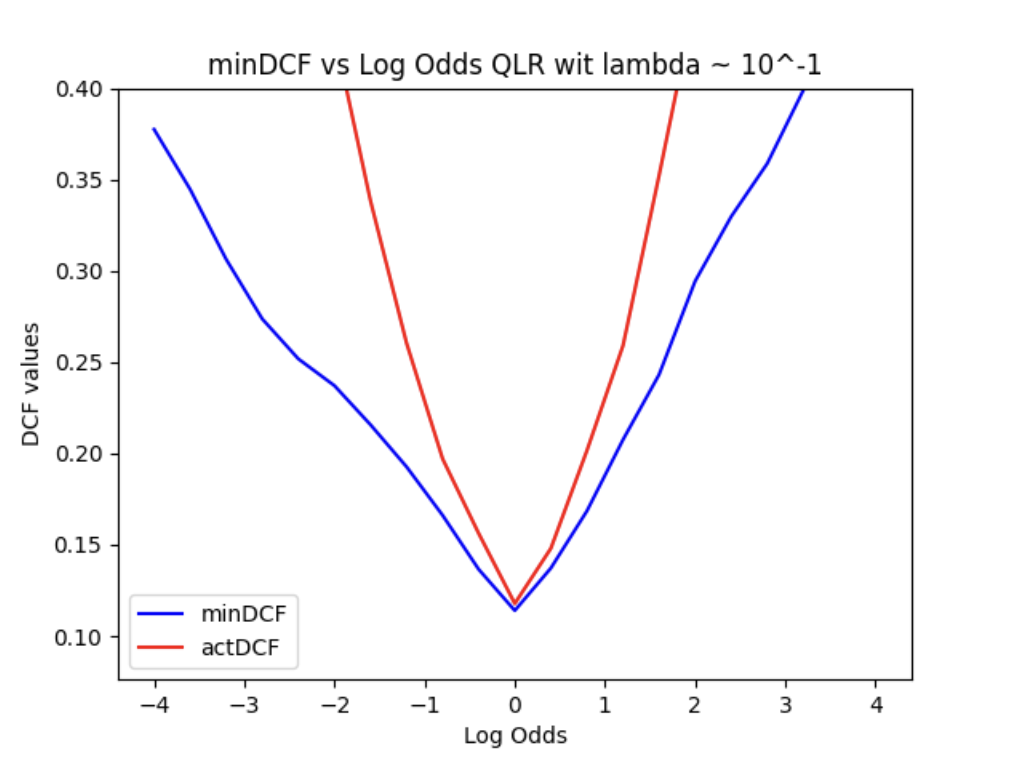
\includegraphics[width=\linewidth]{./img/BestQLR.png}
        % Rimuovi la caption e l'etichetta da qui
    \end{minipage}%
    \begin{minipage}{.3\textwidth}
        \centering
        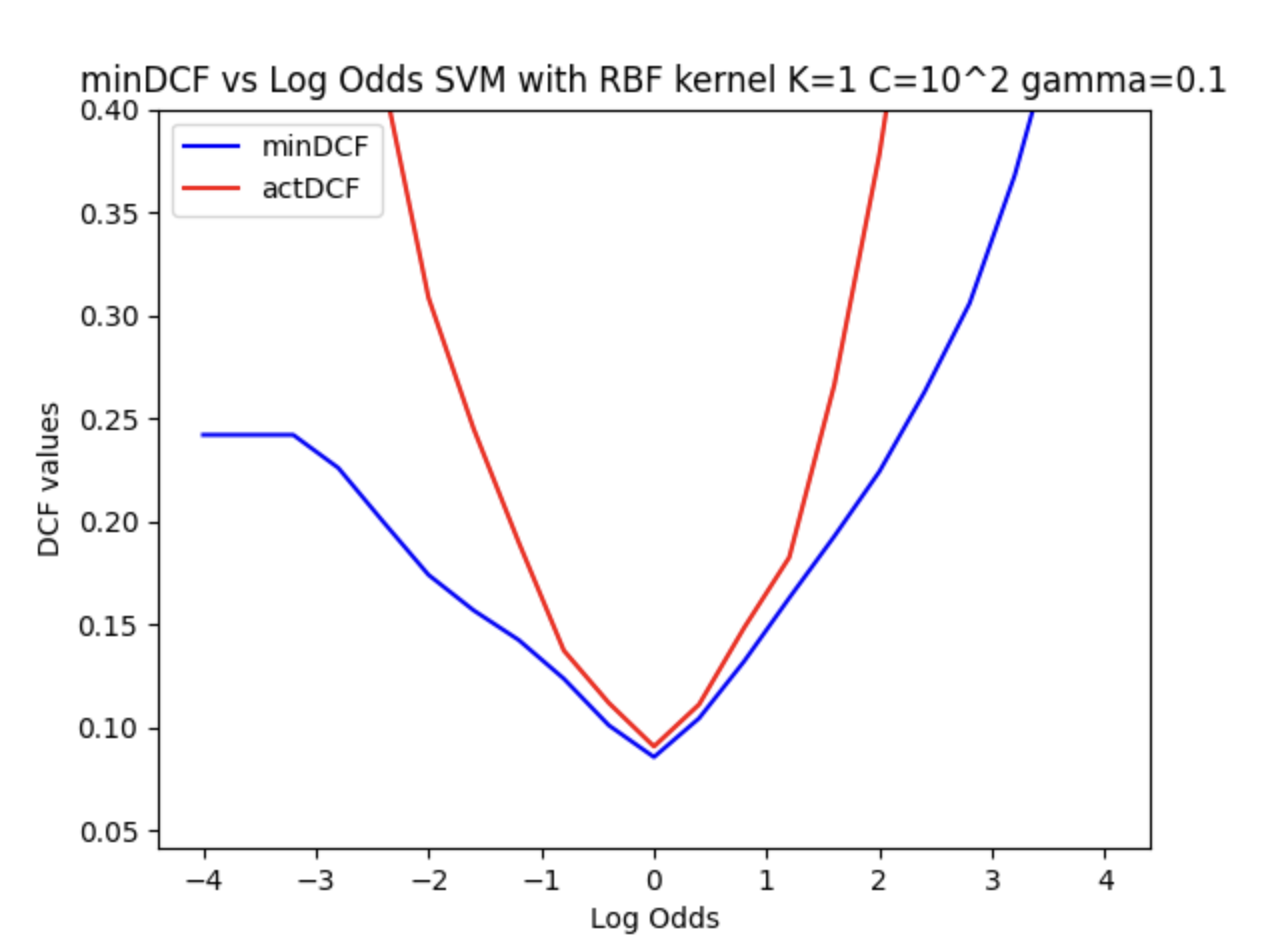
\includegraphics[width=\linewidth]{./img/BestSVM.png}
        % Rimuovi la caption e l'etichetta da qui
    \end{minipage}
    \begin{minipage}{.3\textwidth}
        \centering
        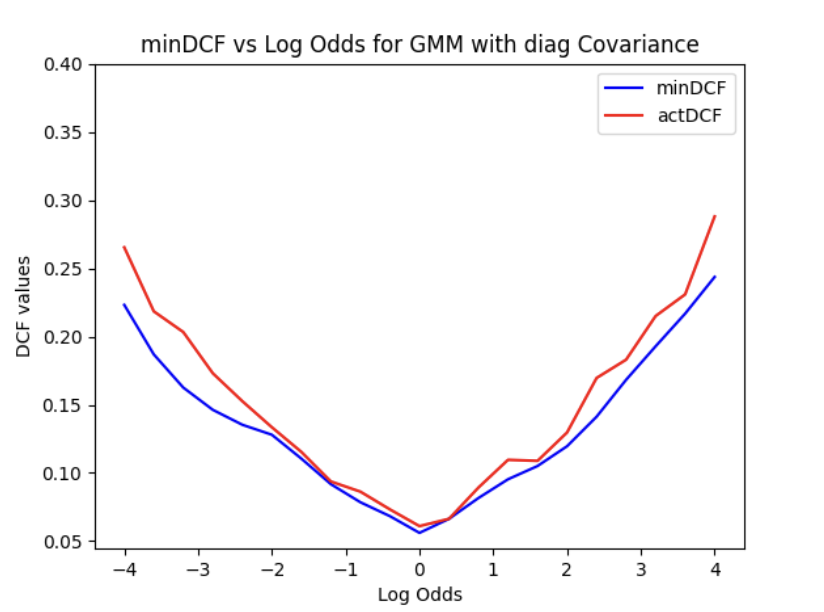
\includegraphics[width=\linewidth]{./img/BestGMM.png}
        % Rimuovi la caption e l'etichetta da qui
    \end{minipage}
    \caption{Analysis best model} % Aggiungi una caption unica qui
    \label{fig:CalAnal} % Aggiungi un'etichetta unica qui
\end{figure}
From the Figure~\Ref{fig:CalAnal} we can see how the selected models while having good performance are not well calibrated, so now we are going to do the calibration.
\subsection{Calibrating Scores for Selected Models}
The metric used to select the best model was the minDCF, however the evaluation is based on theoretical threshold \(t=-log{\frac{\tilde{\pi}}{1-\tilde{\pi}}}\) but there is no guarantee that this threshold is still the optimal one and for this reason an analysis on the score is performed.
We assume that the function f that maps the uncalibrated score to calibrated has the form:
\begin{equation}
    f(s)=\alpha s+\beta
\end{equation}
and f can be interpreted as log-likelihood for the two classes hypotheses:
\begin{equation}
    f(s)=log \frac{f_{S|C}(s|\mathcal{H}_T)}{f_{S|C}(s|\mathcal{H}_F)}=\alpha s+\beta
\end{equation}
and the class posterior probability for prior \(\tilde{\pi}\) corresponds to:
\begin{equation}
    log\frac{P(C=\mathcal{H}_T|s)}{P(C=\mathcal{H}_F|s)}=\alpha s+\beta+log\frac{\tilde{\pi}}{1-\tilde{\pi}}
\end{equation}
By interpreting scores s as samples of a datase a prior weighted logistic regression model can be employed to learn the model parameters over our calibration set. Letting: 
\begin{equation}
    \beta'=\beta+log\frac{\tilde{\pi}}{1-\tilde{\pi}}
\end{equation}
a Logistic Regression model is obtained where \(\alpha\) and \(\beta'\) are the model parameters to be learnt. A prior needs to be specified and will be the one of the target application, but there will be improvements in terms of calibration even on the unbalanced applications. To obtain calibrated scores we will have to compute:
\begin{equation}
    f(s)=\alpha s+\beta=\alpha s+\beta'-log\frac{\tilde{\pi}}{1-\tilde{\pi}}
\end{equation}
Having selected the best models using minDCF as a metric we can now calibrate them to adjust the model predictions so that the predicted probabilities better reflect the actual probabilities of the events. 
\begin{table}[H]
    \centering
    \begin{tabular}{>{\centering\arraybackslash}m{3cm} >{\centering\arraybackslash}m{3cm} >{\centering\arraybackslash}m{3cm}>{\centering\arraybackslash}m{3cm}}
    \hline
    \multicolumn{4}{c}{\textbf{Uncalibrated Models [minDCF/actDCF] }} \\   \hline
    \textbf{QLR} & & 0.243631/0.497167 & \\
    \textbf{SVM} &  & 0.185531/0.361111 & \\
    \textbf{GMM} &  & 0.131240/0.319092 & \\
    \hline
    \hline
    \multicolumn{4}{c}{\textbf{Calibrated Models [minDCF/actDCF] }} \\   \hline
    &\textbf{\(\tilde{\pi}=0.1\)}  &  \textbf{\(\tilde{\pi}=0.5\)} & \textbf{\(\tilde{\pi}=0.9\)} \\ \hline
    \textbf{QLR} & 0.248591/0.272129 & 0.249583/0.260928 & 0.248031/0.265745\\
    \textbf{SVM} & 0.185387/0.189356 & 0.184395/0.202252 & 0.190636/0.202956\\
    \textbf{GMM} & 0.132376/\textcolor{red}{0.151801} & 0.131384/\textcolor{red}{0.151801} & 0.128264/0.155913\\
    \hline
    \textbf{Fusion} & 0.132376/0.156762 & 0.137336/0.163850 & 0.138184/0.173067\\\hline
    \end{tabular}
    \caption{calibrated models}
    \label{tab:Calibrated}
    \end{table}
In the Table~\Ref{tab:Calibrated} we can see the different models after calibration, different priors were used for calibration but the performance was always evaluated on the target application \((\pi_T=0.1)\).
\\
We can see that actDCF improved significantly after calibration, the best results were obtained with the GMM model with prior equal to 0.1 or 0.5.
\begin{figure}[H]
    \centering
    \begin{minipage}{.4\textwidth}
        \centering
        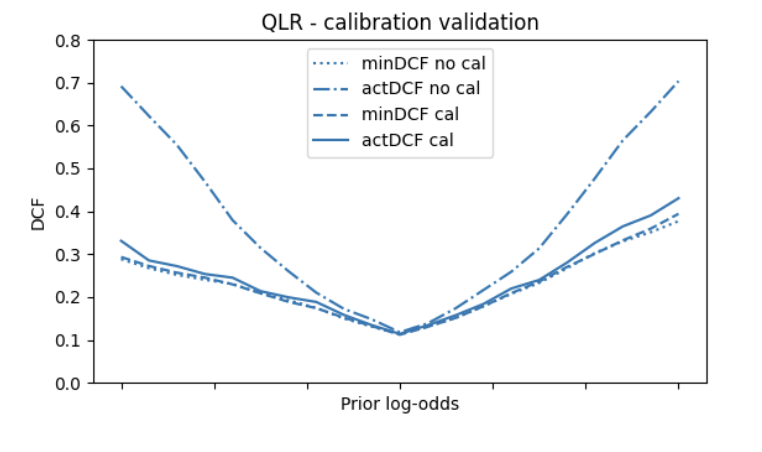
\includegraphics[width=\linewidth]{./img/Cal1.png}
        % Rimuovi la caption e l'etichetta da qui
    \end{minipage}%
    \begin{minipage}{.4\textwidth}
        \centering
        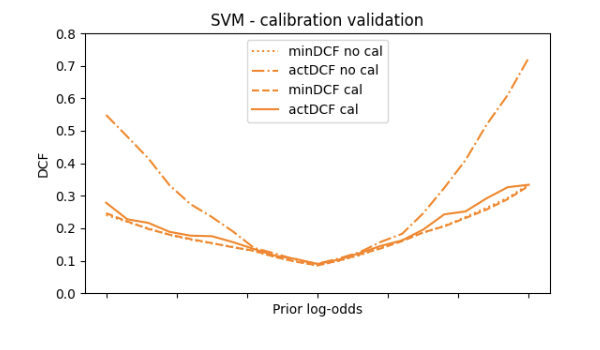
\includegraphics[width=\linewidth]{./img/Cal2.png}
        % Rimuovi la caption e l'etichetta da qui
    \end{minipage}
    \begin{minipage}{.4\textwidth}
        \centering
        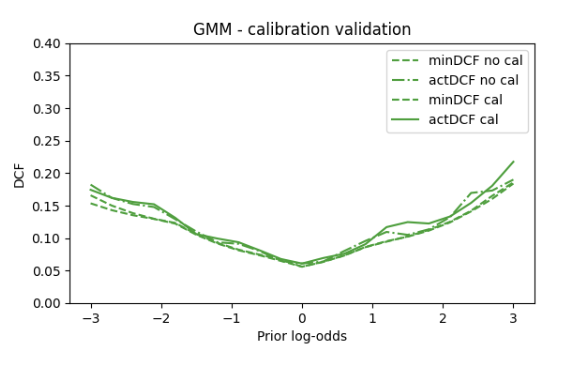
\includegraphics[width=\linewidth]{./img/Cal3.png}
        % Rimuovi la caption e l'etichetta da qui
    \end{minipage}
    \begin{minipage}{.4\textwidth}
        \centering
        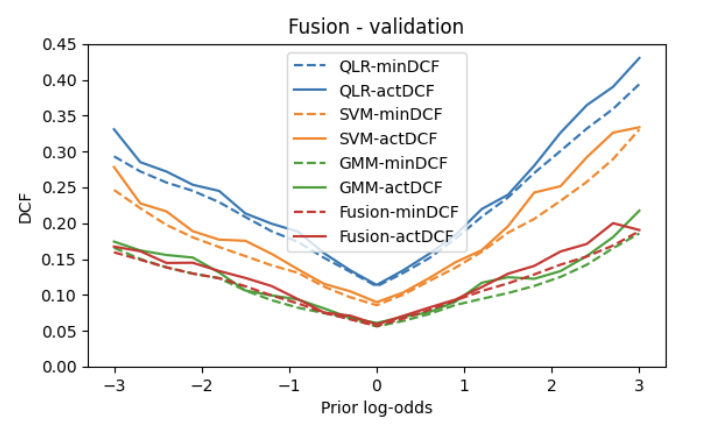
\includegraphics[width=\linewidth]{./img/Cal4.png}
        % Rimuovi la caption e l'etichetta da qui
    \end{minipage}
    \caption{Calibration Model} % Aggiungi una caption unica qui
    \label{fig:CalMod} % Aggiungi un'etichetta unica qui
\end{figure}
\begin{itemize}
    \item We can see from the Bayes error graph how for the other applications as well, not just the target application, there were improvements after the calibration was applied.
    \item It is possible to apply fusion which is used to combine the scores of several models to improve performance, because perhaps one model may not be optimal then one tries to combine several models.\\In our case we can see that the fusion is not greatly improving the performance in fact they are very similar to those obtained by applying the GMM model. Moreover, the fusion does not seem to be optimally calibrated either as the values of minDCF and actDCF still differ by a larger value than the best performing model mentioned above.
\end{itemize}
In conclusion as "delivered" system we choose GMM with Diagonal covariance with the previously mentioned configurations since after comparing it with all the other analyzed models it seems to be the most efficient one to fit our application. In fact as discussed when it was analyzed it seems to be the one most able to fit the distribution of our features managing to discriminate optimally between the different classes compared to the others, this decision was made based on the actDCF and minDCF measurements.
\section{Experimental Results}
\subsection{Evaluation}
Now to evaluate the chosen model we can test it on a new evaluation dataset, no parameters will be calculated on this dataset but we will simply go and test the model we have already trained.\\
From an initial analysis we can infer that the scores are not well calibrated for either the target application or the other possible applications in the evaluation dataset.\\\\
In the Figure~\Ref{fig:Act} we can see what the actDCF values are for the different models before and after calibration, we can we can infer even before calibration that the best model is the one that was chosen. In fact it turns out to have the lowest actDCF compared to the others even before calibration
\begin{figure}[H]
    \centering
    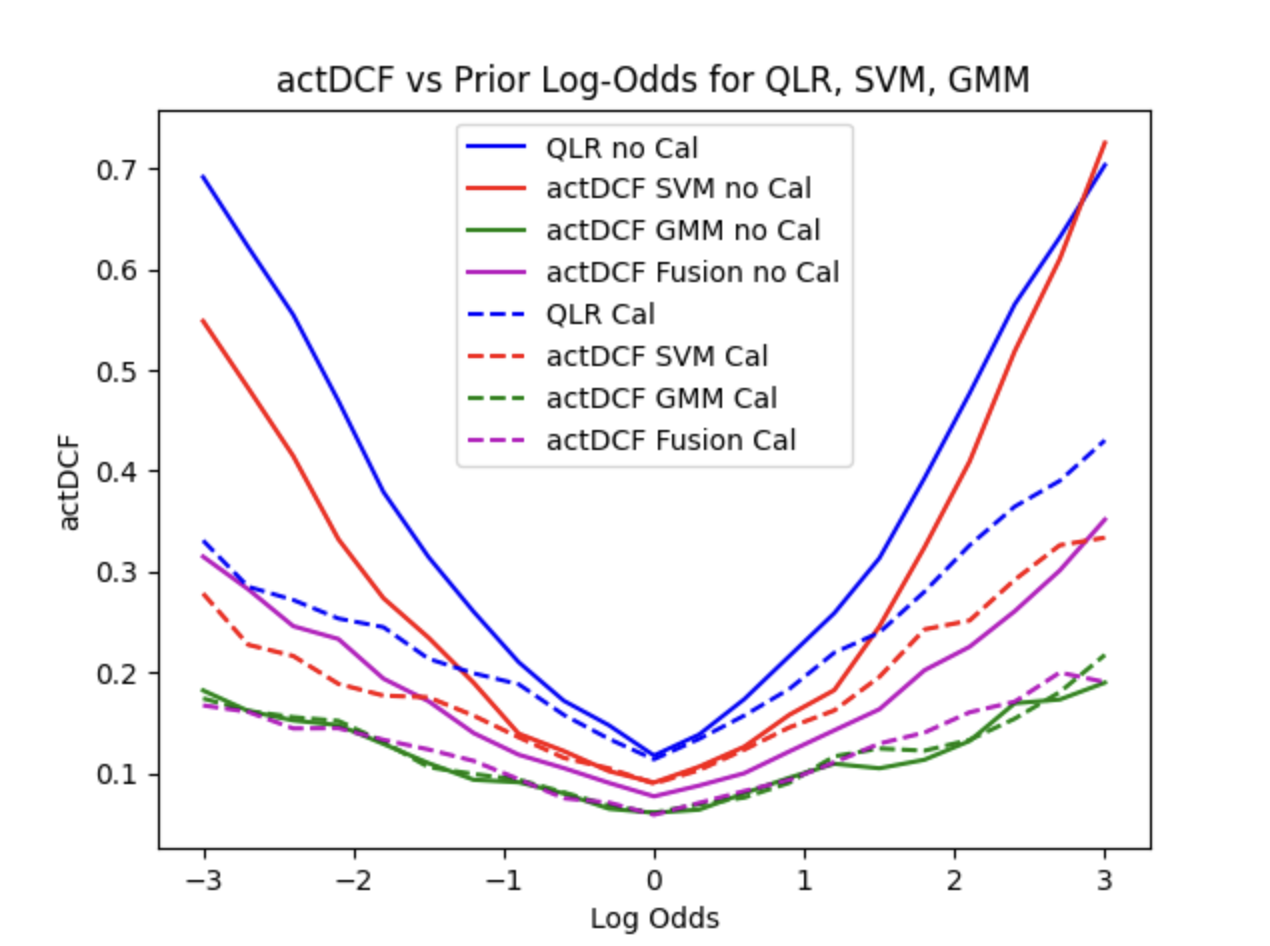
\includegraphics[width=0.45\textwidth]{./img/PlotActDCF.png}
    \caption{Plot various actDCF}
    \label{fig:Act}
\end{figure} 
\begin{table}[H]
    \centering
    \begin{tabular}{>{\centering\arraybackslash}m{3cm} >{\centering\arraybackslash}m{3cm} >{\centering\arraybackslash}m{3cm}>{\centering\arraybackslash}m{3cm}}
    \hline
    \multicolumn{4}{c}{\textbf{Uncalibrated Models [minDCF/actDCF] }} \\   \hline
    \textbf{QLR} & & 0.351473/0.493525 & \\
    \textbf{SVM} &  & 0.265915/0.364114 & \\
    \textbf{GMM} &  & 0.183800/0.369626 & \\\hline
    \textbf{Fusion}& & 0.197922/0.236549 & \\\hline
    \hline
    \multicolumn{4}{c}{\textbf{Calibrated Models [minDCF/actDCF] }} \\   \hline
    &\textbf{\(\tilde{\pi}=0.1\)}  &  \textbf{\(\tilde{\pi}=0.5\)} & \textbf{\(\tilde{\pi}=0.9\)} \\ \hline
    \textbf{QLR} & 0.351473/0.389589 & 0.351473/0.371689 & 0.351473/0.364806\\
    \textbf{SVM} & 0.265915/0.294592 & 0.265915/0.275374 & 0.265915/0.273113\\
    \textbf{GMM} & \textcolor{red}{0.185387/0.205280}& 0.183800/0.202290 & 0.183800/0.210571\\
    \hline
    \textbf{Fusion} &  0.186456/0.204611 & 0.183132/0.205614 &  0.183132/0.208898\\\hline
    \end{tabular}
    \caption{calibrated models to eval dataset}
    \label{tab:CalibratedEval}
    \end{table}
\begin{figure}[H]
    \centering
    \begin{minipage}{.4\textwidth}
        \centering
        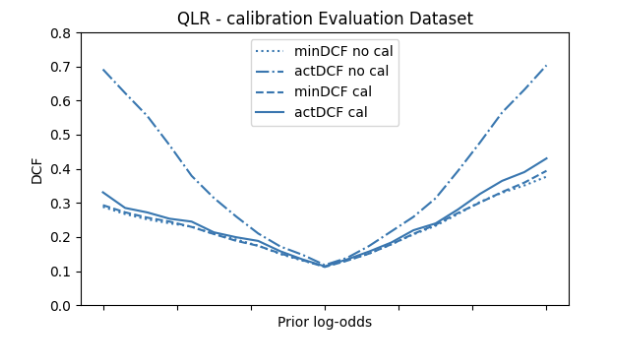
\includegraphics[width=\linewidth]{./img/EVAL1.png}
        % Rimuovi la caption e l'etichetta da qui
    \end{minipage}%
    \begin{minipage}{.4\textwidth}
        \centering
        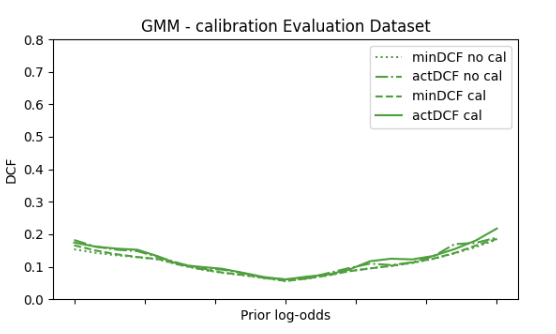
\includegraphics[width=\linewidth]{./img/EVAL2.png}
        % Rimuovi la caption e l'etichetta da qui
    \end{minipage}
    \begin{minipage}{.4\textwidth}
        \centering
        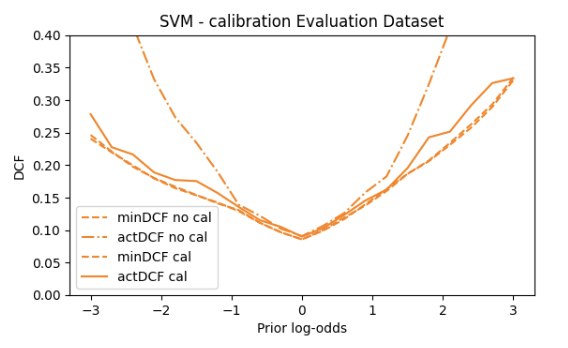
\includegraphics[width=\linewidth]{./img/EVAL3.png}
        % Rimuovi la caption e l'etichetta da qui
    \end{minipage}
    \begin{minipage}{.4\textwidth}
        \centering
        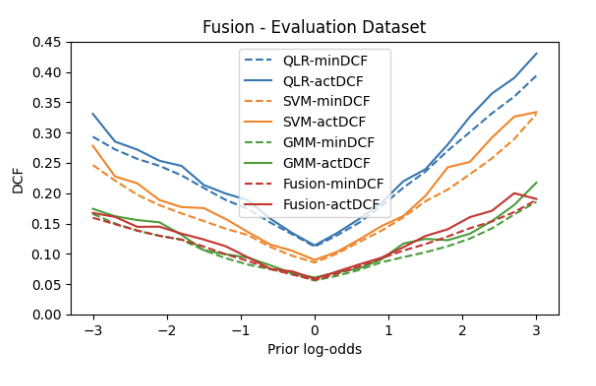
\includegraphics[width=\linewidth]{./img/EVAL4.png}
        % Rimuovi la caption e l'etichetta da qui
    \end{minipage}
    \caption{Calibration Model} % Aggiungi una caption unica qui
    \label{fig:CalEVAL} % Aggiungi un'etichetta unica qui
\end{figure}
\begin{itemize}
    \item After calculating minDCF and actDCF we can say that the results obtained reflect the chosen model, in fact even after this analysis the GMM gives us the best performance along with the fusion of the different models. We can say that both fusion of all trained models and GMM give similar performance.
    \item Again the calibration strategy seems to have worked, in fact we can see that for the GMM model chosen with \(\tilde{\pi}=0.1\) we have a good calibration.
    \item As mentioned earlier we chose the GMM model, this during its training phase was tested with different numbers of components for different classes and using diagonal or full covariance. We can then now evaluate based on the evaluation dataset whether choosing another type of covariance or using a different number of components could have led to a better result. \\
    So by testing other strategies on evaluation we can say that the type of covariance was optimally chosen, in fact diagonal covariance always gives the best results. While the number of components that gives the best results on the evaluation dataset is different we found that the optimal GMM model in this case is with configuration (nc0=4 nc1=16 best minDCF=0.178175). This change of components could be due to the fact that the data distribution is slightly different from the trainining dataset, so in this case different numbers of components could have better generalization ability.
    We can observe the results in Table~\Ref{tab:OtherModel}.
\end{itemize}
\begin{table}[H]
    \centering
    \begin{tabular}{>{\centering\arraybackslash}m{3cm}>{\centering\arraybackslash}m{3cm} >{\centering\arraybackslash}m{3cm} }
    \hline
    \multicolumn{3}{c}{\textbf{Chosen model GMM(Diag,nc0=8,nc1=32)}} \\   \hline
    &\textbf{Uncalibrated} & \textbf{Calibrated}\\\hline
     minDCF/actDCF & 0.183800/0.369626 & 0.185387/0.205280\\
    \hline
    \multicolumn{3}{c}{\textbf{Other model GMM(Diag,nc0=4,nc1=16)}} \\   \hline
    &\textbf{Uncalibrated} & \textbf{Calibrated}\\\hline
     minDCF/actDCF &0.178175/0.367639 & 0.178175/0.196958\\
    \hline
    \end{tabular}
    \caption{calibrated models to eval dataset}
    \label{tab:OtherModel}
    \end{table}
\section{Conclusions}
We can therefore conclude that in general quadratic models give better performance than linear models. And also that the features do not turn out to be particularly correlated as we had mentioned from the beginning since precisely GMM which is the best performing model suggests to us that the features can be considered independent of each other, since using a diagonal covariance matrix assumes that there is no correlation between the different features in the data. This implies that each dimension contributes independently to the overall distribution without interactions with other dimensions.\\\\
Also for this same reason we can conclude that PCA did not give any real improvements, rather the performance remained similar to before the application of it, this could be because the original features are already independent and contribute uniformly to the variance of the data and therefore the application of PCA may not lead to significant improvement in model performance. This is because PCA is useful when there are relationships between features that can be exploited to reduce dimensionality, but if they are already independent, each principal component may end up capturing only a small portion of the total variance, making dimensionality reduction less useful.\\
In the end however, we can conclude that for the target application \(\tilde{\pi}=0.1\) and the choices made on the training dataset also proved useful on the evaluation set when we went to apply them.

\newpage



% ------------------------------------------------------------------------------

\end{document}
